
\documentclass[11pt,a4paper]{article}
\usepackage[utf8x]{inputenc}
\usepackage[T1]{fontenc}
\usepackage[spanish]{babel}
\usepackage{amsmath}
\usepackage{amssymb,amsfonts,textcomp}
\usepackage{color}
\usepackage{array}
\usepackage{multirow}
\usepackage{hhline}
\usepackage{hyperref}
\usepackage{float}
\usepackage{xkeyval}
\usepackage[pdftex]{graphicx}
\usepackage[yyyymmdd,hhmmss]{datetime}
\usepackage[usenames,dvipsnames]{xcolor}
\usepackage{appendix}
\usepackage{listings}
\usepackage{wasysym}
\definecolor{dkgreen}{rgb}{0,0.6,0}
\definecolor{gray}{rgb}{0.5,0.5,0.5}
\definecolor{mauve}{rgb}{0.58,0,0.82}
\definecolor{lstbackground}{rgb}{0.90,0.90,0.90}
% \lstset{frame=tb,
% 	backgroundcolor=\color{lstbackground},
%   language=Bash,
%   aboveskip=3mm,
%   belowskip=3mm,
%   showstringspaces=false,
%   columns=flexible,
%   basicstyle={\small\ttfamily},
%   numbers=none,
%   numberstyle=\tiny\color{gray},
%   keywordstyle=\color{blue},
%   %commentstyle=\color{dkgreen},
%   stringstyle=\color{mauve},
%   breaklines=true,
%   breakatwhitespace=true,
%   extendedchars=true,
%   tabsize=3
% }
\lstset{frame=tb,
	backgroundcolor=\color{lstbackground},
%  language=Bash,
  aboveskip=3mm,
  belowskip=3mm,
  showstringspaces=false,
  columns=flexible,
  basicstyle={\small\ttfamily},
  numbers=none,
%  numberstyle=\tiny\color{gray},
%  keywordstyle=\color{blue},
%  commentstyle=\color{dkgreen},
%  stringstyle=\color{mauve},
  breaklines=true,
  breakatwhitespace=true
  tabsize=4
}
\usepackage{caption}

%\DeclareCaptionFont{black}{ \color{black} }
%\DeclareCaptionFormat{listing}{
%  \colorbox[cmyk]{0.93, 0.95, 0.95,0.01 }{
%    \parbox{\textwidth}{\hspace{15pt}#1#2#3}
%  }
%}
%\captionsetup[lstlisting]{ format=listing, labelfont=black, textfont=black, singlelinecheck=false, margin=0pt, font={bf,footnotesize} }
\captionsetup[lstlisting]{format=plain, font={footnotesize}}
% ...


%\renewcommand{\lstlistingname}{Code}
\usepackage{verbatim}
\begin{comment}
	\hypersetup{
		pdftex, 
		colorlinks=true, 
		linkcolor=blue, 
		citecolor=blue, 
		filecolor=blue, 
		urlcolor=blue, 
	pdftitle={Software Libre}, 
	pdfauthor={Eduardo Grosclaude, Miriam Lechner}, 
	pdfsubject={Documento de la materia Software Libre}, 
	pdfkeywords={Software Libre, Tecnicatura en Administración de Sistemas y 		Software Libre, Universidad Nacional del Comahue}
	}
\end{comment}	



%\addto\captionsspanish {%
%	\def\appendixname{Apéndices}
%}
% Outline numbering
\setcounter{secnumdepth}{1}
% Reset section numbering between parts
\makeatletter
\@addtoreset{section}{part}
\makeatother  
% List styles
\newcommand\liststyleLi{%
\renewcommand\labelitemi{\tiny${\blacksquare}$}
\renewcommand\labelitemii{\tiny${\square}$}
\renewcommand\labelitemiii{\tiny${\circ}$}
\renewcommand\labelitemiv{\tiny${\circ}$}
}
\newcommand\liststyleLii{%
\renewcommand\labelitemi{{\textbullet}}
\renewcommand\labelitemii{${\circ}$}
\renewcommand\labelitemiii{${\blacksquare}$}
\renewcommand\labelitemiv{{\textbullet}}
}
\newcommand\liststyleLiii{%
\renewcommand\labelitemi{{\textbullet}}
\renewcommand\labelitemii{${\circ}$}
\renewcommand\labelitemiii{${\blacksquare}$}
\renewcommand\labelitemiv{{\textbullet}}
}

\liststyleLi

% Page layout (geometry)
\setlength\voffset{-1in}
\setlength\hoffset{-1in}
\setlength\topmargin{2cm}
\setlength\oddsidemargin{2cm}
\setlength\textheight{23.246668cm}
\setlength\textwidth{17.006cm}
\setlength\footskip{26.144882pt}
\setlength\headheight{1.016cm}
\setlength\headsep{0.508cm}
% Footnote rule
\setlength{\skip\footins}{0.119cm}
\renewcommand\footnoterule{\vspace*{-0.018cm}\setlength\leftskip{0pt}\setlength\rightskip{0pt plus 1fil}\noindent\textcolor{black}{\rule{0.25\columnwidth}{0.018cm}}\vspace*{0.101cm}}
% Pages styles
\makeatletter
\newcommand\ps@Standard{
  \renewcommand\@oddhead{{\raggedleft Cabecera \ } {\raggedright \thepage{}}}
  \renewcommand\@evenhead{\@oddhead}
  \renewcommand\@oddfoot{}
  \renewcommand\@evenfoot{\@oddfoot}
  \renewcommand\thepage{\arabic{page}}
}

% \pagestyle{Standard}
\usepackage{fancyhdr}
\pagestyle{fancy}


%%--------------------------------------
% F O N T S 
% \usepackage{dejavu}
%\usepackage{librebaskerville}
%\usepackage{sans}
%\usepackage{libertine}
%\usepackage{lmodern}
%\usepackage{opensans}
%\usepackage{helvet}
%\usepackage{times}

\usepackage{lmodern}
\renewcommand*\familydefault{\sfdefault} %% Only if the base font of the document is to be sans serif


%% LaTeX Preamble - Font choices
%% Each block selects new math, roman (serif), sans serif, and typewriter fonts.
%% Delete or comment out all but one to make your choice.

% Fourier for math | Utopia (scaled) for rm | Helvetica for ss | Latin Modern for tt
%\usepackage{fourier} % math & rm
%\usepackage[scaled=0.875]{helvet} % ss
%\renewcommand{\ttdefault}{lmtt} %tt

% Latin Modern (similar to CM with more characters)
%\usepackage{lmodern} % math, rm, ss, tt
%\usepackage[T1]{fontenc}

% Palatino for rm and math | Helvetica for ss | Courier for tt
%\usepackage{mathpazo} % math & rm
%\linespread{1.05}        % Palatino needs more leading (space between lines)
%\usepackage[scaled]{helvet} % ss
%\usepackage{courier} % tt
%\normalfont
%\usepackage[T1]{fontenc}

% Euler for math | Palatino for rm | Helvetica for ss | Courier for tt
%\renewcommand{\rmdefault}{ppl} % rm
%\linespread{1.05}        % Palatino needs more leading
%\usepackage[scaled]{helvet} % ss
%\usepackage{courier} % tt
%\usepackage{euler} % math
%\usepackage{eulervm} % a better implementation of the euler package (not in gwTeX)

%\normalfont
%\usepackage[T1]{fontenc}

% Times for rm and math | Helvetica for ss | Courier for tt
%\usepackage{mathptmx} % rm & math
%\usepackage[scaled=0.90]{helvet} % ss
%\usepackage{courier} % tt
%\normalfont
%\usepackage[T1]{fontenc}

% !! COMMERICAL FONT !! Lucida Bright (w/expert package)
%\usepackage[T1]{fontenc}
%\usepackage[expert,vargreek,altbullet]{lucidabr}

%% END Font choices
%%---------------------------------------------
% \renewcommand*\familydefault{\sfdefault}
% \pagestyle{Standard}
\usepackage{mdframed}


% footnotes configuration
\makeatletter
\renewcommand\thefootnote{\arabic{footnote}}
\makeatother
\title{Administración de Sistemas Avanzada}
\author{Eduardo Grosclaude, Miriam Lechner}
\date{2016-08-08}
\usepackage{graphicx}

\usepackage{xkeyval}
\usepackage{pifont}
\usepackage{xcolor}
\newcommand{\revisar}[1]{{\color{red}[#1]}}
%\newcommand{\nota}[1]{{\color{red}[#1]}}
%\newcommand{\revisar}[1]{}

\newcommand{\borrador}{
\revisar{\today, \currenttime  -  Material en preparación}
}




\newcommand{\nota}[1]{}

\newcommand{\nonota}[1]{#1}

\newcommand{\quotes}[1]{``#1''}

   
\newcommand{\shade}[1]{\textcolor{black!50}{#1}}

% ancho opcional, por defecto 15cm
% \figura{copyleft}{Símbolo de Copyleft}{copyleft.png}
% \figura[6]{copyleft}{Símbolo de Copyleft}{copyleft.png}
\newcommand{\figura}[4][15]{
 \begin{figure}[htbp] 
 \centering 
 \includegraphics[width=#1cm]{./img/#4} 
 \caption{#3} 
 \label{fig:#2} 
 \end{figure} 
}

% tabla{label}{caption}{columns}{contents}
\newcommand{\tabla}[4]{
 \begin{table} 
 \centering 
 \small
 \begin{tabular}{#3}
 #4
 \end{tabular}
 \caption{#2}
 \label{tab:#1} 
 \end{table} 
}

\usepackage{sectsty}
%\usepackage[compact]{titlesec} 
\definecolor{bl}{rgb}{0.0,0.2,0.6} 
\allsectionsfont{\color{bl}\scshape\selectfont}


\newcommand{\recuadro}[1]{
\begin{minipage}[c]{0.84\textwidth}
\begin{mdframed}
#1
\end{mdframed}
\end{minipage}
}

\newcommand{\code}[1]{\lstinline$#1$}

\hypersetup{colorlinks=true, linkcolor=blue, citecolor=blue, filecolor=blue, urlcolor=blue, 
	pdftitle={Administración de Sistemas Avanzada}, 
	pdfauthor={Eduardo Grosclaude, Miriam Lechner}, 
	pdfsubject={Documento de la materia Administración de Sistemas Avanzada}, 
	pdfkeywords={Administración de Sistemas, Alta Disponibilidad, Virtualización, Almacenamiento, Tecnicatura en Administración de Sistemas y Software Libre, Universidad Nacional del Comahue}}

 
% --------------------------------------------------------------------
\begin{document}

\maketitle

\borrador

\abstract {En este escrito se presenta la descripción y material inicial de la asignatura \textbf{Administración de Sistemas Avanzada}, para la carrera de Tecnicatura Universitaria en Administración de Sistemas y Software Libre, de la Universidad Nacional del Comahue. 

La materia es cuatrimestral en modalidad presencial y las clases son de carácter teórico-práctico, desarrolladas en forma colaborativa. Está preparada con los objetivos generales de capacitar al estudiante para \textbf{implementar configuraciones especiales de almacenamiento, aplicar programación avanzada a la automatización de tareas, y diseñar e implementar estrategias de respaldo y de tolerancia a fallos para servicios críticos}. 
 

\newpage
\emph{}
\newpage

\tableofcontents

\newpage 
\emph{}

%---------- P R E S E N T A C I O N  ---------

\newpage
\part {La asignatura}


\section{Objetivos}
\subsection{De la carrera}
Según el documento fundamental de la Tecnicatura, el Técnico Superior en Administración de Sistemas y Software Libre estará capacitado para:
\begin{itemize}
	\item Desarrollar actividades de administración de infraestructura. Comprendiendo la administración de sistemas, redes y los distintos componentes que forman la
infraestructura de tecnología de una institución, ya sea pública o privada.
	\item Aportar criterios básicos para la toma de decisiones relativas a la adopción de nuevas tecnologías libres.
	\item Desempeñarse como soporte técnico, solucionando problemas afines por medio de la comunicación con comunidades de Software Libre, empresas y desarrolladores de
software.
	\item Realizar tareas de trabajo en modo colaborativo, intrínseco al uso de tecnologías libres.
	\item Comprender y adoptar el estado del arte local, nacional y regional en lo referente a implementación de tecnologías libres. Tanto en los aspectos técnicos como legales.
\end{itemize}
\subsection{De la asignatura}

\begin{itemize}
	\item Saber implementar configuraciones especiales de almacenamiento
	\item Saber aplicar programación avanzada a la automatización de tareas
	\item Saber diseñar e implementar estrategias de respaldo 
	\item Conocer formas de implementar estrategias de tolerancia a fallos para servicios críticos
\end{itemize}


\section{Cursado}
\begin{itemize}
	\item Cuatrimestral de 16 semanas, 128 horas totales
	\item Clases teórico-prácticas presenciales
	\item Promocionable: nota superior a 70/100 en examen o recuperatorio; cuestionarios por 
        temas respondidos. Trabajo práctico obligatorio aprobado.   
\end{itemize}


\section {Contenidos}
\subsection{Contenidos mínimos}
\begin{itemize}
	\item  Instalación sobre configuraciones de almacenamiento especiales. 
	\item  Scripting avanzado. 
	\item  Planificación de tareas. 
	\item  Virtualización. 
	\item  Alta Disponibilidad.
\end{itemize}


\subsection {Programa}
\begin{enumerate}
\item Configuraciones de almacenamiento
\begin{itemize}
	\item   Arquitectura de E/S, Dispositivos de E/S, Filesystems
	\item	Diseños típicos de almacenamiento
	\item	Software RAID, instalación y mantenimiento niveles 0, 1, 10, 5 
	\item	LVM, instalación y mantenimiento	 
\end{itemize}
	
\item Estrategias de respaldo
\begin{itemize}
	\item Copiado y sincronización de archivos
	\item Estrategias y herramientas de backup, LVM snapshots
	\item Control de versiones
\end{itemize}

\item Alta Disponibilidad
\begin{itemize}
	\item Clustering de LB, de HA, de HPC. Conceptos de HA.
	\item Peacemaker/Corosync, DRBD, Clustering de aplicaciones
\end{itemize}

\item Virtualización
\begin{itemize}
	\item Formas de virtualización, herramientas. 
	\item Creación, instalación, migración, eliminación de MV y container.
        \item Container y VM.  
	\item Cloud. IaaS, PaaS, SaaS, etc.
\end{itemize}
\item Scripting avanzado
\begin{itemize}
	\item Accesibilidad. Interfaz gráfica. 
	\item Captura de señales: trap. 
\end{itemize}
\end{enumerate}

\section {Bibliografía inicial}
\begin{itemize}
	\item Kemp, Juliet. Linux System Administration Recipes: A Problem-Solution Approach. Apress, 2009. 
	\item Lakshman, Sarath. Linux Shell Scripting Cookbook Solve Real-World Shell Scripting Problems with over 110 Simple but Incredibly Effective Recipes. Birmingham, U.K.: Packt Pub., 2011. 
	\item Parker, Steve. Shell Scripting Expert Recipes for Linux, Bash, and More. Hoboken, N.J.; Chichester: Wiley; John Wiley, 2011.
	\item K. Kopper, The Linux Enterprise Cluster: build a highly available cluster with commodity hardware and free software. San Francisco: No Starch Press, 2005.
	\item Andrew Beekhof, Pacemaker 1.1 Cluster from scratch. 2016.
	\item R. Pollei, Debian 7 System Administration Best Practices. Birmingham: Packt Publishing, 2013.
	\item T. A. Limoncelli, C. J. Hogan, and S. R. Chalup, The practice of system and network administration. Upper Saddle River, N.J: Addison-Wesley, 2008.
	\item Chen, Peter M., et al., RAID: High-performance, reliable secondary storage. ACM Computing Surveys (CSUR), 1994.
	\item S. van Vugt, Pro Linux high availability clustering. 2014.


\end{itemize}

\subsection{Biblioteca Virtual del MinCyT}

Biblioteca Virtual del MinCyT: \url{http://www.biblioteca.mincyt.gob.ar/libros}.

Títulos accesibles desde la UNC:

\begin{itemize}
	\item C. Wolf and E. M. Halter, Virtualization from the desktop to the enterprise. Berkeley, CA; New York, NY: Apress; Distributed in U.S. by Springer-Verlag New York, 2005; \url{http://rd.springer.com/book/10.1007/978-1-4302-0027-7}.
	\item K. Schmidt, High availability and disaster recovery concepts, design, implementation. Berlin; Springer, 2006; \url{http://rd.springer.com/book/10.1007/3-540-34582-5}.	
\end{itemize}


%----------- M A T E R I A L ---------
\newpage
\part {Scripting Avanzado}
\section{Introducción}
Los contenidos acerca de ``Scripting Avanzado'' serán desarrollados de manera
transversal a toda la materia. En tal sentido, se procederá al análisis y 
modificación de scripts que hagan uso de las tecnologías vistas en los 
restantes contenidos de la materia. 

Por otra parte, haremos foco en las cuestiones de accesibilidad (ver \ref{ref:acces}). Acercando 
el uso de scripts al usuario final (no administrador). 

Con respecto a los contenidos desarrollados específicamente en este apunte, se asumen que el alumno aprobó el cursado de la materia correlativa ``Automatización y scripting''. En tal sentido, la ejercitación básica propuesta en \ref{ref:ejbasica}, debiera ser resuelta a modo de repaso. 

\section {Contenidos}

\begin{enumerate}
\item Comandos básicos de archivos ls, cd, mkdir, cp, mv, rm, ln, patrones de nombres
\item Redirección y piping, comandos head, tail, more, less, grep
\item Variables, ambiente, aritmética
\item Sentencias de control if, for, while, case
\item Funciones
\item Arreglos
\item Expresiones regulares, uso de grep
\item Uso de sort, diff, comm, uniq, cut
\item Uso de cron
\item Otros intérpretes: sed, awk, Perl
\end{enumerate}

\section{Ejercitación básica}\label{ref:ejbasica}

\subsection{Redirección y piping}
\begin{enumerate}
	\item Crear un archivo conteniendo la salida del comando ls
	\item Crear un archivo conteniendo la salida del comando ls -lR /tmp
	\item Obtener las cinco primeras líneas del archivo anterior
	\item Crear un archivo conteniendo las cinco primeras líneas y las cinco  últimas del archivo generado en 2
	\item Crear un archivo conteniendo las primeras cinco líneas de la salida del comando ls -lR /tmp
	\item Usando el anterior, crear un archivo conteniendo esas líneas, numeradas
	\item Crear un archivo conteniendo las últimas cinco líneas de la salida del comando ls -lR /tmp
\end{enumerate}


\subsection {Variables, ambiente}
\begin{enumerate}
	\item Asignar e imprimir el contenido de dos variables
	\item Asignar dos variables, imprimir sus valores, intercambiar sus valores, imprimirlos
	\item Crear un script que imprima un valor que será pasado como argumento
	\item Crear un script que imprima dos valores que serán pasados como argumento
	\item Crear un script que imprima todos los valores que le sean pasados como argumento
\end{enumerate}


\subsection{Sentencias de control}
\begin{enumerate}
	\item 
Imprimir cinco veces "Linux"
	\item 
Imprimir cinco veces el contenido de una variable
	\item 
Imprimir los números de 0 a 5
	\item 
Imprimir los dígitos de -1 a 6
	\item 
Imprimir los números de 0 a 99
	\item 
Imprimir junto al nombre de cada archivo en el directorio actual, su tamaño y su fecha de modificación
	\item 
Copiar los archivos terminados en .txt en archivos con igual nombre pero extensión .bak
	\item 
Renombrar los archivos con extensión .tex que comienzan en ASA reemplazando la partícula ASA con RII
	\item 
Para cada archivo modificado hace más de cinco días en un directorio, mostrar su cantidad de líneas
	\item 
Obtener mediante un cliente de HTTP una lista de archivos cuyos nombres están dados por  una expresión variable y controlada por un lazo
	\item 
De un conjunto de archivos tar, encontrar aquellas versiones de un archivo dado, contenido en ellos, que hayan sido modificadas entre dos fechas dadas.
\end{enumerate}

Las secuencias a continuación son ilustrativas. Se recomienda seguir paso a paso, {\bf comprendiendo cabalmente cada orden}. Incluyendo la interpretación del por qué de los errores mostrados. 

\subsection{Aritmética}
\begin{lstlisting}
$ declare -i num
$ num="hola"
$ echo $num
	0
$ num=5 + 5
	bash: +: command not found
$ num=5+5
$ echo $num
	10
$ num=4*6
$ echo $num
	24
$ num="4 * 6"
$ echo $num
	24
$ num=6.5
	bash: num: 6.5: syntax error in expression (remainder of expression is ".5")
$ i=5; j=$i+1; echo $j
$ i=5; let j=$i+1; echo $j
$ let i=5
$ let i=i+1
$ echo $i
	6
$ let "i = i + 2"
$ echo $i
	8
$ let "i+=1"
$ echo $i
	9
$ i=3
$ (( i+=4 ))
$ echo $i
	7
$ (( i=i-2 ))
$ echo $i
	5
$ let b=2#101; echo $b
$ let h=16#ABCD; echo $h
\end{lstlisting}

\subsection{Arreglos}

\begin{lstlisting}
$ A=(1 2 3 cuatro cinco)
$ echo ${!A[*]}
0 1 2 3 4
$ echo ${A[4]}
cinco
$ echo ${A[*]}
1 2 3 cuatro cinco
$ A[2]='banana'
$ echo ${A[*]}
1 2 banana cuatro cinco
\end{lstlisting}

\subsection{Arreglos asociativos}
\begin{lstlisting}
$ declare -A B
$ B=([francia]='paris' [espana]='madrid' [argentina]='buenos aires')
$ echo ${!B[*]}
espana argentina francia
$ echo ${B[*]}
madrid buenos aires paris
$ echo ${B[francia]}
paris
\end{lstlisting}


\subsection{Here-Documents}

La siguiente técnica permite la creación de archivos de texto dentro de un script. Por ejemplo, podría ser 
necesario crear cierto archivo de configuración en aquellas máquinas de la organización que posean cierto 
software instalado. 

\begin{lstlisting}
$ cat > texto.txt << END
> Hola
> Probando...
> END
$ cat texto.txt
\end{lstlisting}

\subsection{Traps}

El mecanismo de traps, propio del bash, le permite al shell reaccionar frente a ciertos eventos. Por ejemplo,
el desarrollador del script podría necesitar eliminar archivos temporales, creados para fines del script, en caso
de que el usuario decida interrumpir la ejecución (Ctrl+C). 

\begin{lstlisting}
# man 7 signal
# 1 = SIGHUP (Hangup of controlling terminal or death of parent)
# 2 = SIGINT (Interrupted by the keyboard)
# 3 = SIGQUIT (Quit signal from keyboard)
# 6 = SIGABRT (Aborted by abort(3))
# 9 = SIGKILL (Sent a kill command)

trap limpieza 1 2 3 6 9
function limpieza
{
	echo "Recibimos señal - desmantelando..."
	rm -f ${tempfiles}
	echo Finalizando
}
\end{lstlisting}



\section{Casos de uso}

A continuación se presentan un conjunto de problemas a resolver utilizando scripting. Se pretende que el alumno evalúe la posibilidad de resolución, e intente de ser posible el desarrollo de una solución. 

Las siguientes preguntas pretenden ser de ayuda en el comienzo del análisis:
\begin{itemize}
\item ¿Existe alguna herramienta que realice el trabajo? Como regla general, se evita ``re-inventar la rueda''.
\item ¿Es el shell el lenguaje indicado para resolver el problema?
\item ¿Cuál es/son la/s plataforma/s sobre la/s que se ejecutará el script? 
\item ¿Qué shell es el indicado? (relacionado a la pregunta anterior)
\item ¿A quién pertenece el desarrollo?¿Qué licencia se utilizará para el script?
\item ¿Quién será el usuario del script?¿Necesita permisos especiales?
\item ¿Utiliza el script software adicional que no se encuentra usualmente pre-instalado en las computadoras destino?
\item ¿Requiere el script algún tipo de interfaz con el usuario? 
\item ¿Será necesario implementar opciones que modifiquen el comportamiento estándar?
\item ¿Recibirá el script algún tipo de argumento?
\item Dimensionar el problema. ¿Es necesaria algún tipo de modularización?
\item ¿Emite algún tipo de salida? (error o estándar). 
\item ¿Cuáles serán los códigos de error del script? (exit)
\end{itemize}

\subsection{Investigar el sistema}
\begin{enumerate}
	\item 
Modificar la salida del comando blkid para conocer el UUID, el nombre y tipo, y punto de montado, de cada dispositivo de bloques del sistema.
	\item 
Analizar archivos de log buscando conocimiento: duración de sesiones ssh por usuario, mensajes de mail entre usuarios, con histograma por tamaños, etc.
	\item 
Detectar momentos en que la salida de vmstat muestra picos de I/O, procesos corriendo, procesos en espera, uso de swap, etc.
\end{enumerate}


\subsection{Recuperar espacio de almacenamiento}
\begin{enumerate}
	\item Encontrar los diez archivos más grandes en un directorio y sus hijos, imprimirlos junto con su tamaño de mayor a menor.
	\item Encontrar los diez archivos más grandes en un directorio y sus hijos, moverlos a otro directorio (en otro filesystem).
	\item Encontrar los diez archivos más grandes del sistema, imprimir el nombre de usuario dueño.
	\item Agregar al script anterior el envío de notificación por mail al usuario responsable.
		\item 
Encontrar archivos en directorios de usuario con la cadena \quotes{cache} en su nombre e imprimir el uso de disco de cada uno.
	\item 
Idem, enviando nombres a un archivo y usándolo como lista para borrarlos, comprimirlos o moverlos.

\end{enumerate}

\subsection{Networking}
\begin{enumerate}
	\item 
Disparar un aviso cuando se pierde la conectividad a un conjunto de nodos de la red.
	\item 
Analizar la salida del comando netstat para descubrir en qué momento aparece un nuevo puerto abierto y a qué aplicación corresponde.
	\item 
Obtener un log de tráfico y obtener orígenes máximos y mínimos de tráfico, cantidades totales de bytes traficados por interfaz, etc.
	\item 
Recoger estadísticas de espacio en disco, cantidad de procesos, carga de CPU, en diferentes nodos de la red, y centralizarlos en un nodo monitor que presente los resultados.
\end{enumerate}

\subsection{Seguridad}
\begin{enumerate}
	\item 
Detener el script si la identidad del proceso corresponde a root.
	\item 
Solicitar información confidencial (como claves) con video inhibido.
	\item 
Capturar señales para impedir la interrupción del script por BREAK o fallos de ejecución.
	\item 
Utilizar MD5/SHAx para confirmar integridad de archivos.
\end{enumerate}




\subsection{Tratamiento de datos}
\begin{enumerate}
	\item 
Revisar el uso de los comandos cut, join, sort, uniq, comm.
	\item 
Crear script que administra una base de datos en formato CSV.
	\item 
Dado un archivo con una lista de direcciones IP, adjuntarles la resolución inversa de nombres correspondiente.
	\item 
Crear un histograma de accesos por nombre de dominio, a partir de los paquetes registrados en un archivo de log generado por iptables. 
	\item 
Dada una base de datos CSV implementar búsqueda por expresiones regulares.
	\item 
Dada una base de datos CSV implementar proyección sobre un conjunto de campos dados.
	\item 
Convertir un listado de individuos PDF en archivo CSV.
	\item 
Preparar un conjunto de scripts con un único punto de entrada para el administrador. Estos scripts mantendrán un conjunto de bases de datos en formato CSV:
\begin{lstlisting}
alumnos: UID, Username, Apellido, Nombres, NoLegajo, Activo
materias: MID, Nombre, Carrera, Docente
cursadas: UID, MID, Ano, Cuatrimestre
\end{lstlisting}
El dato Activo es booleano. Con estas bases de datos:
\begin{itemize}
	\item 
Listar todas las materias asignadas a un mismo docente.
	\item 
Listar todas las materias cursadas por un alumno.
	\item 
Listar todos los alumnos activos inscriptos en una materia.
	\item 
Listar todos los alumnos que cursan una misma carrera dada durante un año dado.
	\item 
Listar todos los alumnos, agrupados por materia cursada, dentro de cada año. 
	\item 
Listar todos los alumnos de un mismo docente.
	\item 
Dado un alumno por su legajo, consultar su estado Activo/Inactivo.
	\item 
Para aquellos alumnos que hace más de tres años que no se inscriben en ninguna cursada, pasar su dato Activo a falso (Inactivo).
	\item 
Generar un par de archivos en el formato de /etc/passwd y /etc/shadow para todos los alumnos activos.
	\item 
Generar un directorio /home/usuario para cada alumno activo, con UID correspondiente.
\end{itemize}
\end{enumerate}


\section{Accesibilidad para usuarios finales}\label{ref:acces}

La mayoría de los scripts suelen estar orientados al usuario administrador. El uso del shell desde la línea de 
comandos es complejo para la mayoría de los usuarios finales, poco amigable e intuitivo. Sin embargo, en 
ciertos casos puede ser de utilidad, o incluso necesario, que el usuario no administrador utilice ciertos scripts en su tarea diaria. En tal sentido existen herramientas que vinculan el shell script con el entorno gráfico, dando mayor accesibilidad. Se mencionan algunas de ellas a continuación: 

\begin{itemize}
\item xmessage   
\item notify-send 
\item tput / setterm  
\item xdotool
\item dialog 
\item zenity (GNOME) / kdialog (KDE)
\item Algunos navegadores de archivos como Nautilus y Caja, entre otros, permiten extender su funcionalidad incorporando algún método que permita la ejecución de scripts desde la interfaz gráfica. 
\begin{itemize}

\subsection{Ejercitación propuesta}
\begin{enumerate}
	\item 
Preparar un script con interfaz gráfica para copiar archivos seleccionados a una carpeta preestablecida con el fin de obtener un backup periódico de todos sus contenidos.
	\item 
Preparar un script con interfaz gráfica que presente los cinco directorios con mayor ocupación de almacenamiento dentro del home del usuario.
	\item 
Preparar un script con interfaz gráfica que permita escalar en un 50% el 
tamaño de un conjunto de imágenes seleccionadas en un navegador de archivos
a su elección. 
\end{enumerate}

%\newpage
%\part {Configuraciones de Almacenamiento}
%
\section{Contenidos}

En esta sección se desarrollan contenidos relacionados a la gestión de almacenamiento masivo. Incluyendo conceptos y tecnologías. Los temas comprendidos serán: 

\begin{enumerate}
	\item   Arquitectura de E/S, Dispositivos de E/S (particionado), Filesystems (sistemas de archivos). 
	\item	Software RAID (implementación Linux MD), instalación y mantenimiento, niveles 0, 1, 10, 5.
	\item	Manejadores de volúmenes lógicos (implementación de LVM), instalación y mantenimiento
	\item	Diseños típicos de almacenamiento
\end{enumerate}


\section{Dispositivos y sistemas de archivos (filesystems)}

\subsection{Dispositivos lógicos}
Los \textbf{dispositivos lógicos de bloques} están asociados a algún medio de almacenamiento, real o virtual.  Ejemplos de dispositivos de bloques que encontramos con frecuencia son \lstinline$/dev/sda, /dev/sda1, /dev/dvd$, etc. Estos estarán asociados a algún medio, como puede ser un disco  magnético, una memoria de estado sólido o un archivo dentro de un sistema de archivos, por mencionar algunas posibilidades. En general se encontrarán bajo el directorio \lstinline$/dev$ dentro de la FSH (Filesystem Hierarchy).


Los dispositivos lógicos presentan una interfaz que provee direccionamiento random o directo, es decir, sus bloques están numerados y se puede acceder a cualquier bloque con independencia de cuál haya sido accedido anteriormente (operación de \emph{seek}). Pueden directamente contener un sistema de archivos u ofrecer soporte a otros dispositivos virtuales, que los agrupan (como los dispositivos RAID) o en general los utilizan (como los dispositivos snapshot de LVM). Los dispositivos de bloques más usuales con los que nos encontramos son los discos y las particiones, pero es interesante conocer otros dispositivos que están soportados por volúmenes lógicos, archivos, u otros, remotos, que se acceden por medio de la red. 

Desde el punto de vista del administrador/ora de sistemas, los archivos de dispositivo serán el medio para interactuar y gestionar el espacio provisto por el medio virtual o físico que representan. Es así que, por ejemplo, a través de una herramienta como fdisk, podemos dar una estructura al espacio en un disco magnético a través de la creación de una tabla de particiones sobre el dispositivo lógico asociado, por ejemplo: \lstinline$fdisk /dev/sda$ 

\begin{figure}[H]
\begin{center}
        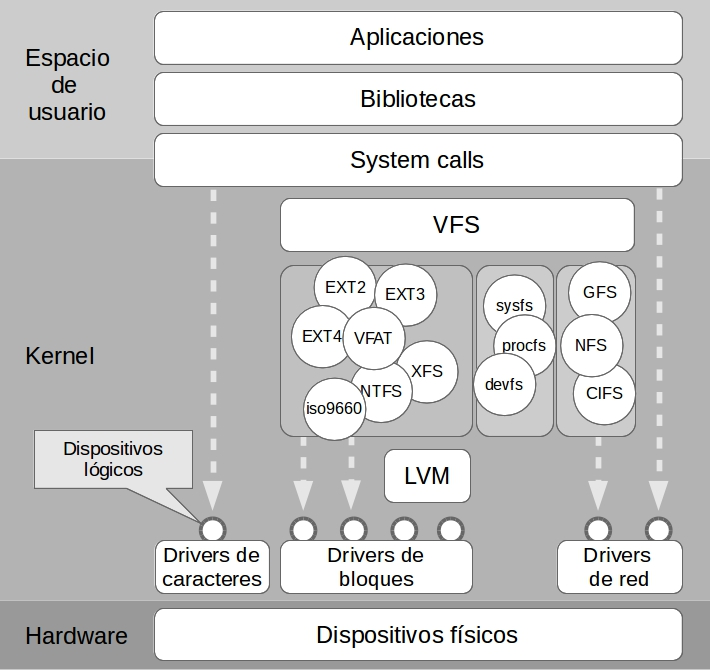
\includegraphics[scale=0.5, angle=0.0]{img/IO.jpg}
        \caption{Esquema IO y dispositivos}
        \label{module}
\end{center}
%\figura[14]{IO}{I/O y dispositivos}{IO.jpg} 
\end{figure}
\subsection{Dispositivos de bucle (loop devices)}

Los dispositivos de bucle (\lstinline$/dev/loop*$) de los 
sistemas GNU/Linux nos permiten \textbf{asociar} 
un archivo de dispositivo (bajo el directorio \lstinline$/dev$) con un 
\textbf{archivo
regular} dentro de un sistema de archivos. Esta funcionalidad nos permite, por 
ejemplo, montar un sistema de archivos que se encuentre contenido dentro del 
archivo regular (como puede ser una imagen ISO), o realizar pruebas simulando
la presencia de múltiples dispositivos. 

Dentro de esta asignatura se desarrollarán tecnologías que permiten la 
combinación de distintos medios de almacenamiento, con diferentes fines, 
por lo que utilizaremos los dispositivos de bucle para simular una 
infraestructura con múltiples discos físicos. 

La siguiente secuencia muestra la forma en que utilizaremos los dispositivos
de bucle con un ejemplo.

\begin{lstlisting}
Creando archivos regulares: 
$ dd if=/dev/zero of=imagen.img bs=1024 count=1024
1024+0 records in
1024+0 records out
1048576 bytes (1.0 MB) copied, 0.00223564 s, 469 MB/s
$ ls -l imagen.img
-rw-r--r-- 1 root root 1048576 Sep  1 11:54 imagen.img

Asociando dispositivos loop a archivos regulares: 
$ losetup /dev/loop0 imagen.img
$ losetup -a
/dev/loop0: [0808]:2260385 (/tmp/imagen.img)

Creando sistema de archivos en el dispositivo asociado: 
$ mkfs -t ext3 /dev/loop0
mke2fs 1.42.8 (20-Jun-2013)

Filesystem too small for a journal
Discarding device blocks:          done                            
Filesystem label=
OS type: Linux
Block size=1024 (log=0)
Fragment size=1024 (log=0)
Stride=0 blocks, Stripe width=0 blocks
128 inodes, 1024 blocks
51 blocks (4.98%) reserved for the super user
First data block=1
Maximum filesystem blocks=1048576
1 block group
8192 blocks per group, 8192 fragments per group
128 inodes per group

Allocating group tables: 0/1	done                            
Writing inode tables: 0/1	done                            
Writing superblocks and filesystem accounting information: 0/1	done

Montando el sistema de archivos para su uso: 
$ mkdir mnt
$ mount -o loop /dev/loop0 mnt
$ df -h mnt
Filesystem      Size  Used Avail Use% Mounted on
/dev/loop0     1003K   17K  915K   2% /tmp/mnt
$ ls -l mnt
total 12
drwx------ 2 root root 12288 Sep  1 11:54 lost+found

Utilizando el sistema de archivos: 
$ ls / > mnt/lista.txt
$ ls -l mnt
total 13
-rw-r--r-- 1 root root   167 Sep  1 11:54 lista.txt
drwx------ 2 root root 12288 Sep  1 11:54 lost+found
$ df -h mnt
Filesystem      Size  Used Avail Use% Mounted on
/dev/loop0     1003K   18K  914K   2% /tmp/mnt

Redimension del archivo regular de base, aumento: 
$ dd if=/dev/zero of=imagen.img bs=1024 count=1024 oflag=append conv=notrunc
1024+0 records in
1024+0 records out
1048576 bytes (1.0 MB) copied, 0.00206669 s, 507 MB/s
$ ls -l imagen.img
-rw-r--r-- 1 root root 2097152 Sep  1 11:54 imagen.img

Indicando al mecanismo de bucle el cambio en el archivo regular: 
$ losetup -c /dev/loop0
$ losetup -a
/dev/loop0: [0808]:2260385 (/tmp/imagen.img)
/dev/loop1: [0005]:5178 (/dev/loop0)

Redimension del sistema de archivos contenido en el dispositivo: 
$ umount mnt
$ e2fsck -fp /dev/loop0
/dev/loop0: 12/128 files (0.0% non-contiguous), 39/1024 blocks
$ resize2fs /dev/loop0
resize2fs 1.42.8 (20-Jun-2013)
Resizing the filesystem on /dev/loop0 to 2048 (1k) blocks.
The filesystem on /dev/loop0 is now 2048 blocks long.

Puesta en funcionamiento del cambio: 
$ mount /dev/loop0 mnt
$ df -h mnt/
Filesystem      Size  Used Avail Use% Mounted on
/dev/loop0      2.0M   18K  1.9M   1% /tmp/mnt

\end{lstlisting}

\subsection{Sistemas de archivos}

Los sistemas de archivos son piezas de software fundamentales del sistema operativo que 
permiten el uso de los dispositivos de almacenamiento por parte de los usuarios
del sistema. Sin sistemas de archivos la organización del espacio de almacenamiento sería una tarea ardua. El sistema de archivos será entonces el software que 
permite la gestión del espacio disponible en un dispositivo, a través de la 
creación de estructuras lógicas (metadatos) dentro del espacio de almacenamiento, que permiten la gestión del mismo. Estas estructuras son las que se crean 
dentro del espacio de almacenamiento al utilizar comandos como \lstinline$mkfs$. Los metadatos ocupan un espacio en sí mismos, es por esto que, al crear
el sistema de archivos, el tamaño utilizable resultante es menor al espacio
real disponible. La elección del tipo de sistema de archivos también 
impactará en este sentido, habrá sistemas de archivos con metadatos más 
complejos y otros con metadatos más simples. 

Existen múltiples sistemas de archivos, con características diversas y finalidades distintas. Todos ellos tienen como fin gestionar el espacio. Encontramos sistemas simples, como FAT, hasta extremadamente complejos como puede ser btrfs. 

La elección de un sistema de archivos particular depende del uso y las
características del almacenamiento subyacente, así como del soporte provisto
por el sistema operativo. Elegiremos sistemas de archivos
distintos para un pendrive, que para un disco magnético. Evaluaremos si 
se alojarán archivos grandes o pequeños, etc. A continuación presentamos un 
conjunto de preguntas que deberíamos responder al momento de elegir 
el software más adecuado: 

\begin{itemize}
\item ¿Sobre qué medio físico voy a crear dicho sistema?
\item ¿Cuál es el tamaño del sistemas de archivos?
\item ¿Cuál es el tamaño esperable de los archivos a almacenar?
\item ¿Es esperable que el sistema de archivos crezca?
\item ¿Tasa anual de crecimiento?
\item ¿Performance del sistema de archivos a largo plazo? (fragmentación).
\item ¿Cuál es el estado de desarrollo del software en el sistema
operativo destino?
\item ¿Puedo migrar de un sistema de archivos a otro?
\item El sistema de archivos considerado ¿está soportado en el sistema
operativo destino?
\end{itemize}


\section{RAID}

Los \emph{arrays} RAID (Redundant Array of Independent Disks) son dispositivos virtuales creados como combinación de dos o más dispositivos físicos. El dispositivo virtual resultante puede contener un filesystem. 

Los diferentes modos de combinación de dispositivos, llamados niveles RAID, ofrecen diferentes características de redundancia y performance. Un array RAID con redundancia ofrece protección contra fallos de dispositivos. 

Los dispositivos Software RAID de Linux son creados y manejados por el driver \lstinline{md} (Multiple Device) y por eso suelen recibir nombres como \lstinline{md0}, \lstinline{md1}, etc.

 
\begin{itemize}
	\item Redundancia para tolerancia a fallos
	\item Mejoramiento de velocidad de acceso
	\item Hardware RAID, Fake RAID, Software RAID
	\item Niveles RAID
	\item RAID Devices
	\item Spare disks, faulty disks
\end{itemize}



\subsection {Niveles RAID}

\begin{description}
	\item [Linear mode] Dos o más dispositivos concatenados. La escritura de datos ocupa los dispositivos en el orden en que son declarados. 
Sin redundancia.
Mejora la performance cuando diferentes usuarios acceden a diferentes secciones del file system, soportadas en diferentes dispositivos.
	\item [RAID-0] Las operaciones son distribuidas (\emph{striped}) entre los dispositivos, alternando circularmente entre ellos. Cada dispositivo se accede en paralelo, mejorando el rendimiento. Sin redundancia. 
	\item [RAID-1]
Dos o más dispositivos replicados (\emph{mirrored}), con cero o más \emph{spares}. 
Con redundancia. Los dispositivos deben ser del mismo tamaño. Si existen \emph{spares}, en caso de falla o salida de servicio de un dispositivo, el sistema reconstruirá automáticamente una réplica de los datos sobre uno de ellos. 
En un RAID-1 de $N$ dispositivos, pueden fallar o quitarse hasta $N-1$ de ellos sin afectar la disponibilidad de los datos. 
Si $N$ es grande, el bus de I/O puede ser un cuello de botella (al contrario que en Hardware RAID-1). El scheduler de Software RAID en Linux asigna las lecturas a aquel dispositivo cuya cabeza lectora está más cerca de la posición buscada. 
	\item [RAID-4] No se usa frecuentemente. Usado sobre tres o más dispositivos. Mantiene información de paridad sobre un dispositivo, y escribe sobre los restantes en la misma forma que RAID-0. El tamaño del array será $(N-1)*S$, donde $S$ es el tamaño del dispositivo de menor capacidad en el array. 
Al fallar un dispositivo, los datos se reconstruirán automáticamente usando la información de paridad. El dispositivo que soporta la paridad se constituye en el cuello de botella del sistema. 


\item [RAID-5]
Utilizado sobre tres o más dispositivos con cero o más \emph{spares}. El tamaño del dispositivo RAID será $(N-1)*S$. La diferencia con RAID-4 es que la información de paridad se distribuye entre los dispositivos, eliminando el cuello de botella de RAID-4 y obteniendo mejor performance en lectura. Al fallar uno de los dispositivos, los datos siguen disponibles. Si existen \emph{spares}, el sistema reconstruirá automáticamente el dispositivo faltante. Si se pierden dos o más dispositivos simultáneamente, o durante una reconstrucción, los datos se pierden definitivamente. RAID-5 sobrevive a la falla de un dispositivo, pero no de dos o más. 
La performance en lectura y escritura mejora con respecto a un solo dispositivo. 

\item [RAID-6]
Usado sobre cuatro o más dispositivos con cero o más \emph{spares}. La diferencia con RAID-5 es que existen dos diferentes bloques de información de paridad, distribuidos entre los dispositivos participantes, mejorando la robustez. El tamaño del dispositivo RAID-6 es $(N-2)*S$. Si fallan uno o dos de los dispositivos, los datos siguen disponibles. Si existen \emph{spares}, el sistema reconstruirá automáticamente los dispositivos faltante. La performance en lectura es similar a RAID-5, pero la de escritura no es tan buena.

\item [RAID-10]
Combinación de RAID-1 y RAID-0 completamente ejecutada por el kernel, más eficiente que aplicar dos niveles de RAID independientemente. Es capaz de aumentar la eficiencia en lectura de acuerdo a la cantidad de dispositivos, en lugar de la cantidad de pares RAID-1, ofreciendo un 95\% del rendimiento de RAID-0 con la misma cantidad de dispositivos. Los \emph{spares} pueden ser compartidos entre todos los pares RAID-1.

\begin{comment}

\item [FAULTY]

Nivel especial de RAID que sirve para debugging del array por inyección de fallos de lectura y escritura. Sólo permite un dispositivo. Simula fallos a bajo nivel, permitiendo analizar comportamiento en caso de fallos de sector en lugar de fallos de discos.
\end {comment}

\end{description}

\subsection {Modos de operación}

\begin{description}
	\item [Create] 
	Creación de un array nuevo con superblocks por cada dispositivo.
	 \item [Assemble]
	Ensamblar dispositivos componentes previamente creados para conformar un dispositivo RAID activo. Los componentes pueden especificarse en el comando o ser identificados por scanning. 
	\item [Follow o Monitor]
Monitorizar un dispositivo RAID y actuar en caso de eventos interesantes. No se aplica a RAID niveles 0 ni linear, ya que sus componentes no poseen estados (\emph{failed}, \emph{spare}, \emph{missing}). 

	\item [Build]
	Construir un array sin superblocks por dispositivo (para expertos).
	\item [Grow]
	Extender o reducir un array, cambiando el tamaño de los componentes activos (RAID 1, 4, 5 y 6) o cambiando el número de dispositivos activos en RAID1.
	\item [Manage]
	Manipular componentes específicos de un array, como al agregar nuevos dispositivos \emph{spare} o al eliminar dispositivos \emph{faulty}.
	\item [Misc]
	Toda otra clase de operaciones sobre arrays activos o sus componentes.

\end{description}

\subsection{Construcción y uso de un array RAID-1}



Crear particiones en ambos discos, tipo fd (Linux RAID autodetect)
\begin{lstlisting}
fdisk /dev/sdb; fdisk /dev/sdc
\end{lstlisting}

Crear el array
\begin{lstlisting}
mdadm --create /dev/md0 --level=1 --raid-devices=2 /dev/sdb1 /dev/sdc1
watch cat /proc/mdstat
\end{lstlisting}

Usar el array
\begin{lstlisting}
mkfs -t ext3 /dev/md0
mkdir /datos
mount -t ext3 /dev/md0 /datos
cp /etc/hosts /datos
ll /datos
\end{lstlisting}

Examinar el array
\begin{lstlisting}
cat /proc/mdstat
cat /proc/partitions
mdadm --examine --brief --scan --config=partitions
mdadm --examine /dev/sdc
mdadm --query --detail /dev/md0
\end{lstlisting}

Crear script de alerta
\begin{lstlisting}
cat > /root/raidalert
#!/bin/bash
echo $(date) $* >> /root/alert
^D
chmod a+x /root/raidalert
\end{lstlisting}

Monitorear el arreglo con script de alerta
\begin{lstlisting}
mdadm --monitor -1 --scan --config=partitions --program=/root/raidalert
\end{lstlisting}

Crear configuración
\begin{lstlisting}
cat > /etc/mdadm.conf
DEVICE=/dev/sdb1 /dev/sdc1
ARRAY=/dev/md0 devices=/dev/sdb1,/dev/sdc1
PROGRAM=/root/raidalert
\end{lstlisting}

Establecer tarea periódica de monitoreo
\begin{lstlisting}
crontab -e
MAILTO=""
*/2 * * * * /sbin/mdadm --monitor -1 --scan 
\end{lstlisting}

Declarar un fallo
\begin{lstlisting}
mdadm /dev/md0 -f /dev/sdb1
cat /root/alert
\end{lstlisting}

Quitar un disco del array
\begin{lstlisting}
mdadm /dev/md0 -r /dev/sdb1 
cat /root/alert
\end{lstlisting}

Reincorporar el disco al array
\begin{lstlisting}
mdadm /dev/md0 -a /dev/sdb1 
cat /proc/mdstat
cat /root/alert
\end{lstlisting}

Destruir el array
\begin{lstlisting}
mdadm --stop /dev/md0
\end{lstlisting}

\subsection {Temas de práctica}
\begin{enumerate}
	\item ¿Qué marcas, modelos y precios de tarjetas controladoras RAID puede encontrar? ¿Con qué capacidades?
	\item ¿Qué diferencias hay entre Software RAID y Hardware RAID?
	\item ¿Qué niveles RAID ofrecen redundancia? ¿Contra qué eventos protege esta redundancia? ¿Contra qué eventos \emph{no} protege esta redundancia? 
	\item El uso de un dispositivo RAID, ¿es un reemplazo efectivo para las políticas y actividades de backup?
	\item ¿Cuáles niveles RAID ofrecen mejor velocidad de trabajo? ¿De qué factores depende la ventaja en performance de los diferentes niveles RAID entre sí y con respecto al uso de una única unidad de disco?
	\item ¿Cuál es la diferencia entre los niveles Linear RAID y RAID 0? ¿Qué clase de redundancia ofrece cada uno? ¿Contra qué eventos protege?
	\item Preparar un arreglo linear RAID sobre dos dispositivos loop. Observe qué relación tiene el espacio disponible en el dispositivo con los archivos que soportan los dispositivos loop.
	\item Preparar un arreglo linear RAID sobre dos discos extra agregados al equipo. 
	\item Preparar un arreglo RAID nivel 0 sobre dos discos extra agregados al equipo. 	
	\item ¿Puede medir la diferencia en performance entre los dispositivos de   los ejercicios anteriores, de linear RAID y de nivel 0? ¿Tiene sentido esta medición cuando el equipo es una máquina virtual? 
	\item Preparar un RAID nivel 1 sobre dos discos extra. Inyectar un fallo en uno de los discos. Agregar un nuevo disco e incorporarlo al RAID. Observar la sincronización del dispositivo.
	\item Como antes, preparar un RAID nivel 1 sobre dos discos extra, pero con una unidad \emph{spare}. Inyectar un fallo en uno de los discos y observar el comportamiento del dispositivo. 
	\item Retire el disco fallado y compruebe en qué estado queda el dispositivo.
	\item Vuelva a agregar el disco y compruebe en qué estado queda el dispositivo. 
	\item ¿Con qué comandos se investiga el estado de un dispositivo RAID? ¿Cómo se sabe cuándo un dispositivo RAID está activo o en modo degradado? ¿Cómo se sabe cuándo un dispositivo está fallado, activo, sincronizando?
	\item ¿Cuál es la forma de convertir en dispositivo RAID 1 un filesystem ya existente?
	\item ¿Cómo se puede adaptar el comportamiento de un RAID 1 a una situación con discos asimétricos (uno más rápido que el otro)?
	
\end{enumerate}



\section{Administración de LVM}
\subsection{Introducción a  LVM}
\label{sub:introLVM}
El soporte habitual para los file systems de servidores son los discos magnéticos, particionados según un cierto diseño definido al momento de la instalación del sistema. Las particiones se definen a nivel del hardware. El conjunto de aplicaciones y servicios del sistema utiliza los filesystems que se instalan sobre estas particiones. 

Las particiones de disco son un concepto de hardware, y dado que las unidades de almacenamiento se definen estáticamente al momento del particionamiento, presentan un problema de administración a la hora de modificar sus tamaños. 


El diseño del particionamiento se prepara para distribuir adecuadamente el espacio de almacenamiento entre los diferentes destinos a los que se dedicará el sistema. Sin embargo, es frecuente que el patrón de uso del sistema vaya cambiando, y el almacenamiento se vuelva insuficiente o quede distribuido en forma inadecuada. La solución a este problema implica normalmente el re-particionamiento de los discos, operación que obliga a desmontar los filesystems y a interrumpir el servicio. Para redimensionar una partición, normalmente es necesario el reinicio del equipo, con la consiguiente interrupción del servicio en producción (es especial si hablamos de particiones en uso por parte del sistema). 


La alternativa consiste en interponer una capa intermedia de software entre el hardware crudo, con sus particiones, y los filesystems sobre los que descansan los servicios. Esta capa intermedia está implementada por Logical Volume Manager (LVM). LVM es un subsistema orientado a flexibilizar la administración de almacenamiento, al interponer una capa de software que implementa dispositivos de bloques lógicos por encima de las particiones físicas. 

Usando LVM, el almacenamiento queda estructurado en capas, y las unidades lógicas pueden crearse, redimensionarse, o destruirse, sin necesidad de reinicio, desmontar ni detener el funcionamiento del sistema. Con LVM pueden definirse por software contenedores de filesystems, de límites flexibles, que admiten el redimensionamiento \quotes{en caliente}, es decir sin salir de actividad, mejorando la disponibilidad general de los servicios.

Con LVM pueden agregarse unidades físicas mientras el hardware lo permita, extendiéndose dinámicamente las unidades lógicas y redistribuyendo el espacio disponible a conveniencia. Presenta también otras ventajas como la posibilidad de extraer \emph{snapshots} o instantáneas de un filesystem en funcionamiento (para obtener backups consistentes a nivel de filesystem), y manipular con precisión el mapeo a unidades físicas para aprovechar características del sistema (como \emph{striping} sobre diferentes discos).


% subsubsection  (end)




\subsection{Componentes de LVM}
\label{sub:compLVM}
En la terminología LVM, los dispositivos de bloques entregados al sistema LVM se llaman PV (physical volumes). Cualquier dispositivo de bloques escribible puede convertirse en un PV de LVM. Esto incluye particiones de discos y dispositivos múltiples como conjuntos RAID. Los PVs se agrupan en VGs (volume groups) que funcionan como \emph{pools} de almacenamiento físico. De cada pool pueden extraerse a discreción LVs (logical volumes), que se comportan nuevamente como dispositivos de bloques, y que pueden, por ejemplo, alojar filesystems. Estos serán los usuarios finales de la jerarquía (Fig. \ref{fig:jerLVM}).


\figura{jerLVM}{Jerarquía de componentes LVM}{LVM.png}


\recuadro{
Conviene tener en mente la jerarquía de los siguientes elementos:
\begin{description}
	\item [Volumen físico o PV (physical volume)] Es un contenedor físico que ha sido agregado al sistema LVM. Puede ser una partición u otro dispositivo de bloques adecuado.
	\item [Grupo de volúmenes o VG (volume group)] Es un pool o repositorio de espacio conformado por uno o varios PVs. Un VG ofrece un espacio de almacenamiento virtualmente continuo, cuyo tamaño corresponde aproximadamente a la suma de los PVs que lo constituyen. Los límites entre los PVs que conforman un VG son transparentes.
	\item [Volumen lógico o LV (logical volume)] Es una zona de un VG que ha sido delimitada para ser usada por otro software, como por ejemplo un filesystem. Los tamaños de los LVs dentro de un VG no necesariamente coinciden con los de los PVs que los soportan.
\end{description}
}



\subsection {Uso de LVM}
Los pasos lógicos para utilizar almacenamiento bajo LVM son: 
\begin{itemize}
	\item Crear uno o más PVs a partir de particiones u otros dispositivos.
	\item Reunir los PVs en un VG con lo cual sus límites virtualmente desaparecen.
	\item Particionar lógicamente el VG en uno o más LVs y utilizarlos como normalmente se usan las particiones.
\end{itemize}

\begin{comment}
\figura[8]{LVMcomponentes}{Volúmenes físicos (PV), Grupos de Volúmenes (VG) y Volúmenes Lógicos (LV)} {LVM-componentes.jpg}
\end{comment}

El sistema LVM incluye comandos para realizar estas tareas y en general administrar todas estas unidades. Con ellos se puede, dinámicamente:
\begin{itemize}
	\item Redimensionar LVs de modo de ocupar más o menos espacio dentro del VG.
	\item Aumentar la capacidad de los VGs con nuevos PVs sin detener el sistema.
	\item Mover LVs a nuevos PVs, más rápidos, sin detener el sistema.
	\item Usar \emph{striping} entre PVs de un mismo VG para mejorar las prestaciones.
	\item Tomar una instantánea o \emph{snapshot} de un LV para hacer un backup del filesystem contenido en el LV.
	\item Tomar una instantánea como medida preventiva antes de una actualización o modificación.
\end{itemize}



Los comandos tienen nombres con los prefijos \lstinline$pv$, \lstinline$vg$, \lstinline$lv$, etc. Además, el comando \lstinline$lvm$ ofrece una consola donde se pueden dar esos comandos y pedir ayuda.

	


% subsubsection  (end)

\subsection{Redimensionamiento de volúmenes}
\label{sub:redimVol}
Una vez creado un LV, su capacidad puede ser reducida o aumentada (siempre que exista espacio extra en el VG que lo contiene) con los comandos \lstinline$lvreduce$ o \lstinline$lvresize$. 
Si el LV redimensionado contuviera un filesystem, éste también debe ser redimensionado en forma acorde. 
\begin{itemize}
	\item Si un filesystem debe ser extendido, primero debe extenderse el LV que lo contiene. 
	\item Si un filesystem va a ser reducido, luego debe reducirse el LV que lo contiene (en caso contrario, el espacio extra se desperdicia). 
	\item Si un LV va a ser reducido, primero debe reducirse el filesystem que contiene.
	\item Si un LV va a ser extendido, luego debe extenderse el fileystem que contiene (en caso contrario, el espacio extra se desperdicia). 
	\item Si un LV que va a ser reducido está ocupado en un cierto porcentaje, la reducción del LV sólo puede llevarse a cabo en forma segura en dicho porcentaje. 
\end{itemize}

Este redimensionamiento del filesystem puede ser hecho por el administrador con un comando separado, o automáticamente en el momento de redimensionar el LV.

\subsubsection {Redimensionamiento automático}
La herramienta \lstinline$resize2fs$, que modifica el tamaño de un filesystem, es capaz de extender los filesystems sin necesidad de desmontar. Sin embargo, para reducir el tamaño de un filesystem, será necesario desmontarlo. 

Aún más conveniente que \lstinline$resize2fs$ es la opción -r de los comandos lvreduce y lvresize. Esta opción tiene en cuenta el tamaño final del LV que se está redimensionando, y modifica el tamaño del filesystem contenido adecuadamente, todo en la misma secuencia de operación. 

\subsubsection {Indicación del nuevo tamaño}
La opción -L (o --size) indica el nuevo tamaño del LV en bytes, con sufijos M (mega), G (giga), T (tera), etc.

En el comando \lstinline$lvresize$, si el tamaño se indica con un prefijo de signo más o menos, significa que el tamaño debe aumentar o disminuir en la cantidad que se indica a continuación. En cambio, si el tamaño no lleva prefijo, significa que esa cantidad debe ser el tamaño final del LV. En el comando \lstinline$lvreduce$ sólo tiene sentido el signo menos (ejemplos en Cuadro \ref{tab:resize1}).

\tabla{resize1}{Tamaños con y sin signo}{c|l|c}{
Original &Comando & Final\\
\hline
& \lstinline$lvresize -r -L 10G vg0/lv0$  &  10GB \\
50 GB &  \lstinline$lvresize -r -L -10G vg0/lv0$  &  40GB \\
 &  \lstinline$lvreduce -r -L -10G vg0/lv0$  &  40GB \\
& \lstinline$lvresize -r -L +10G vg0/lv0$  &  60GB \\
\hline
}




\subsubsection {Bytes y extents}
El nuevo tamaño para un LV puede darse en múltiplos del byte (MB, GB, TB...) o en \emph{extents} (la unidad mínima de asignación de bloques de LVM, por defecto 4 MB). La opción -L (o --size) indica el tamaño deseado en bytes, y -l (o --extents) en extents.

Al usar extents, se puede opcionalmente indicar el tamaño deseado en términos relativos del tamaño del VG, del LV, o del espacio libre dentro del VG. Por ejemplo, supongamos que:

\begin{itemize}
	\item el volumen lógico \lstinline$vg0/lv0$ mide 40 GB, 
	\item el VG \lstinline$vg0$ que lo contiene mide 100 GB, 
	\item el espacio del VG \lstinline$vg0$ no ocupado por el LV \lstinline$vg0/lv0$ está libre.
\end{itemize}


Bajo estas condiciones, diferentes comandos \lstinline$lvresize$ tienen los efectos que se ven en el Cuadro \ref{tab:res2}.

\tabla{res2}{Uso de extents}{c|l|c|l}{
Original		& Comando 	& Final 	& \\
\hline
 		&\lstinline$lvresize -r -l 1000 vg0/lv0$  &  4 GB & 1000 extents = 1000 * 4 MB = 4 GB\\
		&\lstinline$lvresize -r -l +1000 vg0/lv0$  &  44 GB & 40 GB + 4 GB = 44 GB\\
		&\lstinline$lvresize -r -l +100\%LV vg0/lv0$  &  80 GB & Se duplica el tamaño del LV\\
	40 GB	&\lstinline$lvresize -r -l -10\%LV vg0/lv0$  &  36 GB & Se reduce el LV en un 10\%\\
		&\lstinline$lvresize -r -l +10\%VG vg0/lv0$  &  50 GB & Se agrega un 10\% del total del VG\\
		&\lstinline$lvresize -r -l +10\%FREE vg0/lv0$  &  46 GB & Se agrega un 10\% del espacio libre del VG\\
		&\lstinline$lvresize -r -l +10\%ORIGIN vg0/snap$  &  14 GB & Si el snapshot era de 10 GB (un 25\% \\
& &	&	 del LVO), lo extiende en un 10\% del LVO\\
\hline
}


\subsection{Snapshots y backups}
\label{sub:snapshots}

Un snapshot es un LV virtual, especialmente preparado, asociado a un LV original cuyo estado se necesita \quotes{congelar} para cualquier propósito de mantenimiento. Una vez creado el snapshot, mediante un mecanismo de \emph{copy-on-write (o COW)}, LVM provee una instantánea o vista inmutable del filesystem original, aunque éste se actualice. Una vez creado el LV virtual de snapshot, sus contenidos son estáticos y permanentemente iguales al LV original. Puede ser montado y usado como un filesystem corriente. El snapshot es temporario y una vez utilizado se descarta. 

La motivación principal del mecanismo de snapshots es la extracción de copias de respaldo. Durante la operación del sistema, las aplicaciones y el kernel leen y escriben sobre archivos, y por lo tanto el filesystem pasa por una sucesión de estados. Una operación de backup que se desarrolle concurrentemente con la actividad del filesystem no garantiza la consistencia de la imagen obtenida, ya que archivos diferentes pueden ser copiados en diferentes momentos, bajo diferentes estados del filesystem. Como consecuencia, la imagen grabada no necesariamente representa un estado concreto de la aplicación; y esto puede dar lugar a problemas al momento de la recuperación del backup. 

Hay muchos escenarios posibles de inconsistencia. Algunos ejemplos son:
\begin{itemize}
	\item Una aplicación que mantiene un archivo temporario en disco con modificaciones automáticas y periódicas (por ejemplo, \lstinline$vi$). 
	\item Aplicaciones que mantienen conjuntos de archivos fuertemente acoplados (bases de datos compuestas por tablas e índices en archivos separados).
	\item Una instalación de un paquete de software, que suele afectar muchos directorios del sistema. 
\end{itemize}

Una solución consiste en \quotes{congelar} de alguna forma el estado del filesystem durante la operación de copia (por ejemplo, desmontándolo). Con LVM, gracias al mecanismo de \emph{COW}, esta instantánea puede ser obtenida sin detener la operación del LV original, o sea sin afectar la disponibilidad del servicio. La operación con el filesystem del LV origen (LVO) no se interrumpe, ni modifica en nada la conducta de las aplicaciones que lo estén usando. 

\subsubsection {Dimensionamiento del snapshot}

Para la creación de un snapshot de un LVO se necesita contar con espacio extra disponible (no utilizado por ningún LV) dentro del mismo VG al cual pertenece el LVO. Este espacio extra no necesita ser del mismo tamaño que el LVO. Normalmente es suficiente un 15\% a 20\% del tamaño del LV original. Si el VG no tiene suficiente espacio, debe extenderse previamente.

No es fácil determinar con precisión el tamaño del snapshot, ya que debe ser suficiente para contener todos los bloques modificados en el LVO durante el tiempo en que se use el snapshot; y este conjunto de bloques puede ser variable, dependiendo del patrón de uso del LVO y del medio hacia el cual se pretende hacer el backup (otro disco local, un servidor en la red local, un servidor en una red remota, una unidad de cinta, tienen diferente ancho de banda y diferente demora de grabación).

En el Cuadro \ref{tab:res2} hay un ejemplo de redimensionamiento del LV snapshot en función del tamaño del LVO.

\subsubsection{Creación de snapshots}
\label{ssub:snapcreate}

Crear un snapshot es preparar un nuevo LV, virtual, con un filesystem virtualmente propio, que se monta en un punto de montado diferente del original (Fig. \ref{fig:snap1}). 

\figura[8]{snap1}{Un LVO y su snapshot}{LVM-snapshot-1.jpg}
 
A partir de este momento se pueden hacer operaciones de lectura y escritura en ambos filesystems separadamente, con efectos distintos en cada caso. 

% subsubsection  (end)

\subsubsection{Lectura y escritura del LVO}
\label{ssub:lvorw}
Los snapshots son creados tomando un espacio de bloques de datos (la tabla de excepciones) dentro del mismo VG del LVO. Mientras un bloque no sea modificado, las operaciones de lectura lo recuperarán del LVO. Pero, cada vez que se modifique un bloque del LVO, la versión original, sin modificar, de dicho bloque, será copiada en el snapshot (Fig. \ref{fig:snap2}). 

\figura[8]{snap2}{Escritura de un bloque del LVO}{LVM-snapshot-2.jpg}
 
\subsubsection{Lectura y escritura del snapshot}
\label{ssub:snaprw}
De esta manera, el snapshot muestra siempre los contenidos originales del LVO (Fig. \ref{fig:snap3}), salvo que se modifiquen por alguna operación de escritura en el snapshot.

\figura[8]{snap3}{Lectura de un bloque desde el snapshot}{LVM-snapshot-3.jpg}

Los LVs pueden declararse R/O o R/W. En LVM2, los snapshots son R/W por defecto.  Al escribir sobre un filesystem de un LV snapshot R/W, se grabará el bloque modificado en el espacio privado del snapshot sin afectar el LVO (Fig. \ref{fig:snap4}). Al eliminar el snapshot, todas las modificaciones hechas sobre el mismo desaparecen. 

\figura[8]{snap4}{Escritura sobre el snapshot}{LVM-snapshot-4.jpg}



\subsection {Creación de backups con snapshots}
\begin{enumerate}
	\item Se crea un snapshot del LV de interés.
	\item Se monta el snapshot en modo R/O sobre un punto de montado conocido. 
	\item Se copian los archivos del snapshot con la técnica de backup que se desee. 
	\item Se verifica la integridad del backup.
	\item Si la verificación no fue satisfactoria, se repite el backup.
	\item En caso satisfactorio, el snapshot se destruye con \lstinline$lvremove <ID del snapshot>$.  

\end{enumerate}

\begin {comment}
--------------------------------------------
, en un momento en que el filesystem esté en estado consistente (por ejemplo, al arranque del sistema, mientras aún no ha sido montado, o mientras los servicios están administrativamente detenidos).
--------------------------------------------
\end{comment}

\subsection{Uso preventivo de snapshots}
El mecanismo de snapshots ofrece la posibilidad de recuperar el estado original del LVO al efectuar operaciones que pueden afectar críticamente la integridad u operatividad del sistema, tales como pruebas de instalación, modificación de configuraciones, etc. 

Como se ha visto, el conjunto de datos almacenados en un snapshot está formado por bloques que, o bien provienen del LVO original, en su estado anterior a ser modificados (Fig. \ref{fig:snap2}), o bien, son bloques de archivos que fueron modificados mediante operaciones regulares de escritura sobre el filesystem localizado en el snapshot y montado en modo R/W (Fig. \ref{fig:snap4}). 

En ambos casos, este conjunto de bloques alojados en el snapshot puede volver a ser aplicado sobre el LVO (o \emph{revertido}) con la opción \lstinline$--merge$ del comando \lstinline$lvconvert$. Este comando restituye (\emph{roll-back}) al LVO todos sus bloques originales, que fueron grabados temporariamente en el espacio de excepciones del snapshot, y \emph{luego destruye el snapshot}. 

\subsubsection{Reversión de snapshots}
Ahora bien, al ser revertido el snapshot sobre el LVO:
\begin{itemize}
	\item Si no ha habido ninguna operación de escritura sobre el filesystem del snapshot, el LVO \emph{vuelve al estado original} al momento de ser tomado el snapshot. 
	\item Si, en cambio, existen archivos en el snapshot que han sido modificados, al revertir el snapshot el LVO \emph{cambia}, asumiendo las modificaciones que se hayan hecho en el snapshot. 
\end{itemize}

El resultado, para el LVO, será completamente diferente en uno y otro caso. Ambas propiedades pueden aprovecharse para recuperar el estado después de una modificación que no ha sido satisfactoria, con una de las dos técnicas siguientes.


\begin{description}
\item [Técnica 1] Con esta técnica, las modificaciones se realizan sobre el filesystem del LVO y en caso necesario se revierten usando el snapshot intacto. 
\begin{enumerate}
	\item Crear el snapshot del LVO, con espacio suficiente para registrar las modificaciones que se piensa hacer.
	\item Ejecutar las operaciones críticas (instalar, actualizar, modificar) sobre el LVO.
	\item Verificar el resultado.
	\begin{itemize}
		\item Si el resultado fue satisfactorio, destruir el snapshot con \lstinline$lvremove <ID snapshot>$. 
		\item Si el resultado no fue satisfactorio, recuperar el estado original del LVO con el comando \lstinline$lvconvert --merge <ID del snapshot>$.
	\end{itemize}
	\item El snapshot ha sido eliminado.
\end{enumerate}
\end{description}

\begin{description}
\item [Técnica 2] Con esta técnica se deja el LVO fuera de línea, intacto, y se trabaja sobre el snapshot montado en modo R/W. 
\begin{enumerate}
	\item Crear el snapshot del LVO, con espacio suficiente para registrar las modificaciones que se piensa hacer.
	\item Desmontar el LVO y montar en su lugar el snapshot.
	\item Ejecutar las operaciones críticas (instalar, actualizar, modificar) sobre el snapshot.
	\item Verificar el resultado.
	\begin{itemize}
		\item Si fue satisfactorio, se vuelcan las modificaciones al LVO con  \lstinline$lvconvert --merge <ID del snapshot>$. 
		\item Si no fue satisfactorio, se elimina el snapshot.
	\end{itemize}
	\item Finalmente, en uno u otro caso, el snapshot ha sido eliminado, y se vuelve a montar el LVO en su lugar.
\end{enumerate}
\end{description}



\subsection{Eliminación del snapshot}
\label{ssub:snapdel}

El snapshot debe ser destruido al finalizar el backup o terminar de usarlo, ya que, al obligar a  copiar  cada bloque del LVO que se modifica, representa un  costo en performance del sistema de I/O. Por lo demás, el snapshot se define con una cierta capacidad, que al ser excedida hace inutilizable el snapshot completo.

% subsubsection  (end)

\subsection{Ejemplos LVM}
\label{sub:ejemplosLVM}

Creación de Physical Volumes (PV)
\begin{lstlisting}
fdisk /dev/sdb
pvcreate /dev/sdb1 /dev/sdb2
pvdisplay
\end{lstlisting}

Creación de Volume Groups (VG)
\begin{lstlisting}
vgcreate vg0 /dev/sdb1 /dev/sdb2
vgdisplay
\end{lstlisting}

Creación de Logical Volumes (LV)
\begin{lstlisting}
lvcreate --size 512M vg0 -n lvol0
lvcreate -l 50%VG vg0 -n lvol1
lvcreate -l 50%FREE vg0 -n lvol2
lvdisplay vg0
\end{lstlisting}

Examinar LVM
\begin{lstlisting}
pvs
vgs
lvs
pvscan
vgscan
lvscan
\end{lstlisting}

Uso de volúmenes
\begin{lstlisting}
mkfs -t ext3 /dev/vg0/lvol0
mkdir volumen
mount /dev/vg0/lvol0 volumen
cp *.gz volumen
ls -l volumen
\end{lstlisting}

Extensión de un volumen
\begin{lstlisting}
umount /dev/vg0/lvol0
lvextend --size +1G vg0/lvol0
mount /dev/vg0/lvol0 volumen
resize2fs /dev/vg0/lvol0 
\end{lstlisting}

Agregar un disco al sistema
\begin{lstlisting}
fdisk /dev/hdd
pvcreate /dev/hdd1
vgextend vg0 /dev/hdd1
lvextend --size +1G vg0/lvol0 
ext2online /dev/vg0/lvol0 
\end{lstlisting}

Snapshot de un volumen
\begin{lstlisting}
lvcreate -s -n snap --size 100M vg0/lvol0
ls -l /dev/vg0
mkdir volumen-snap
mount /dev/vg0/snap volumen-snap
ls -l volumen-snap/
rm volumen/archivo1.tar.gz volumen/archivo2.tar.gz
ls -l volumen-snap/
\end{lstlisting}

Destruir un snapshot
\begin{lstlisting}
lvremove vg0/snap
\end{lstlisting}
% subsubsection Ejemplos LVM (end)

\subsection{Temas de práctica}
\begin{enumerate}
	\item Crear una partición, convertirla en PV, crear un VG y definir un LV \lstinline$lv0$ dentro del mismo dejando un 25\% del espacio libre. Crear un filesystem sobre el LV, montarlo y utilizarlo para administrar archivos.
	\item Definir un nuevo LV \lstinline$lv1$ en el mismo VG creado anteriormente, ocupando la totalidad del espacio del VG.
	\item Crear otra partición en el mismo u otro medio de almacenamiento, convertirla en PV y adjuntarla al VG del ejercicio anterior. Examinar el resultado de las operaciones con los comandos de revisión correspondientes. 
	\item Extender el LV \lstinline$lv1$ para ocupar nuevamente la totalidad del espacio del VG extendido. Crear un filesystem sobre el LV, montarlo y utilizarlo para administrar archivos.
	\item Modificar los tamaños de ambos LVs, extendiendo uno y reduciendo el otro. Recordar que al reducir un LV se debe primero reducir el filesystem alojado, y que para extender un filesystem se debe primero extender el LV que lo aloja. Comprobar que los filesystems alojados siguen siendo funcionales.
	\item Supongamos que, al querer crear un snapshot de un LV, el administrador recibe un mensaje de error diciendo que el VG no cuenta con espacio disponible. Sugiera un método para enfrentar este problema usando LVM.
	\item Dado un LV, poner en práctica las técnicas de creación de snapshot para a) obtener un backup, y b) realizar modificaciones sobre el LV volviendo después al estado original.  
\end{enumerate}


\section{SMART}

La tecnología SMART (Self-Monitoring, Analysis and Reporting Technology) es un conjunto de funciones útiles para verificar la confiabilidad de los discos y predecir sus fallos. Estas funciones se incorporan en casi todos los discos rígidos electromecánicos ATA y SCSI actuales, así como en los de estado sólido. Los discos dotados de SMART pueden ejecutar varias clases de tests sobre sí mismos, y reportar sus resultados.

La interfaz SMART puede ser usada por el hardware o desde software adecuado. Normalmente el firmware BIOS puede hacer uso de SMART ejecutando un chequeo de salud de los discos al inicio del equipo y denunciando problemas potenciales o existentes. El paquete de software \lstinline{smartmontools} permite utilizar las funciones de SMART de los discos desde varios sistemas operativos.

\subsection{Atributos}
La tecnología SMART incorpora sensores de ciertas variables físicas, y contadores de una cantidad de eventos relevantes, que describen la historia y el estado de los discos. El firmware SMART del disco almacena estos datos, llamados atributos, en memoria no volátil situada en el mismo disco, y los actualiza automáticamente. Cada disco, dependiendo del fabricante, del modelo y del nivel de la especificación ATA al cual adhiere, mantiene un conjunto de estos atributos. Se numeran entre 1 y 253, y tienen nombres específicos. Se dice que dos terceras partes de los fallos de los discos pueden ser predichos observando los valores de determinados atributos. También puede determinarse si un disco ha llegado al fin de su vida útil en base a estos valores.

Los atributos SMART tienen un \quotes{valor crudo} o \emph{raw} y un \quotes{valor normalizado}. El valor crudo de cada atributo tiene una interpretación dada en ciertas unidades. En el caso del atributo 12 (Fig. \ref{fig:smart}), llamado \lstinline{power_cycle_count}, por ejemplo, el valor crudo es simplemente un entero que representa la cantidad de veces que el disco ha sido activado; para otros atributos, debe interpretarse como una temperatura en grados Celsius (atributo 194,  \lstinline{temperature_celsius}), una cantidad de horas (atributo 9, \lstinline{power_on_hours}), etc. Estos valores de interpretación natural corren, lógicamente, sobre diferentes escalas. El \quotes{valor normalizado} de un atributo, por el contrario, está siempre entre 1 y 254, y se obtiene del valor crudo mediante una función matemática que es computada por el firmware del mismo disco. Estos valores normalizados, al ser comparados con determinados umbrales, denuncian la aparición de problemas. El fabricante del disco, que es quien conoce los detalles de construcción y funcionamiento del disco, provee el algoritmo para computar la función de normalización y el valor del umbral para cada atributo. SMART almacena el valor normalizado actual y el \quotes{peor valor} histórico (el menor valor normalizado obtenido desde la primera puesta en operación del disco hasta el momento actual) de cada atributo. 

\subsection{Diagnósticos}
SMART agrupa los atributos en dos clases: \emph{Old Age} y \emph{Pre-failure}. Los primeros sirven para diagnosticar cuándo un disco ha llegado al término de su vida útil, y los segundos para diagnosticar fallos efectivos o inminentes de los discos.
Si, en algún caso, el valor normalizado de un atributo resulta inferior o igual a su umbral, entonces el diagnóstico depende del tipo del atributo. Si un disco tiene un atributo de tipo Old Age cuyo valor normalizado es inferior al umbral, entonces se concluye que el disco ha superado su vida útil según el diseño del producto. Si un atributo es de tipo Pre-failure y su valor normalizado es inferior al umbral, entonces se anuncia un fallo inminente en 24 horas\footnote{En un estudio publicado por Google (Eduardo Pinheiro et al., Failure Trends in a Large Disk Drive Population. USENIX V, 2007) se muestra evidencia, obtenida sobre una población muy grande, de que los fallos de discos están correlacionados sobre todo con dos variables mantenidas por SMART: los errores de superficie (scan errors) y los eventos de reubicación de sectores (reallocation count).}. Si el \quotes{peor valor}  de un atributo de tipo Pre-failure es menor que el umbral, es indicio seguro de que el disco ha presentado un fallo en algún momento anterior.


\figura{smart}{Parte del informe SMART}{SMART.png}


\subsection{Tests}

SMART provee tres clases de tests, que pueden hacerse sin riesgo durante la operación normal del sistema y no causan errores de lectura ni de escritura. La primera categoría se llama \emph{online testing}, y no tiene efecto sobre la performance del dispositivo. La segunda categoría se llama \emph{offline testing}, y puede causar una degradación de la performance, aunque en la práctica esto es raro porque el disco suspende el test cada vez que hay actividad de lectura o escritura. Estas dos primeras categorías de tests deberían más bien llamarse \quotes{adquisición de datos}, ya que simplemente se ocupan de actualizar constantemente los valores de los atributos. 
La tercera categoría es un test propiamente dicho, y se llama \emph{self test}. 
% subsection  (end)

\subsection{Paquete smartmontools}

Comprende dos componentes: el daemon smartd y la interfaz de usuario smartctl. El daemon smartd habilita las funciones de SMART en los discos y consulta su estado cada cierto intervalo. Los parámetros de operación de smartd se indican en su archivo de configuración \lstinline{/etc/smartd.conf}. La herramienta smartctl sirve para consultar el estado de los discos y ejecutar tests.



%\newpage
%\part {Estrategias de Respaldo}
%\section{Copias de respaldo}
\subsection{Establecimiento de una política de copias de respaldo}
La estrategia de copias de respaldo (backup en inglés)  implica mucho más que la decisión 
de qué herramienta particular utilizar (tar, rsync, etc.)  y dónde almacenar las copias.  A continuación 
se enumeran algunos de los aspectos principales que el administrador deberá contemplar a la hora de definir 
la política de copias de respaldo de la organización.

\begin{itemize}
	\item Propósitos y requerimientos legales, confidencialidad, etc.
	\item Archivos a respaldar 
	\begin{itemize}
		\item Archivos de sistema, de los usuarios, de las aplicaciones
		\item Vuelcos de bases de datos, formatos portables.
	\end{itemize}	
	\item Dinámica de los archivos
	\begin{itemize}
		\item Estáticos o volátiles 
		\item Tasa de crecimiento 
	\end{itemize}
	\item Período de cobertura (ventana de seguridad)
	\item Esquema y política de respaldo 
	\begin{itemize}
		\item Quién es responsable
		\item Frecuencia y alcance de cada operación de backup
		\item Diarios, semanales
		\item Completos, diferenciales, incrementales
	\end{itemize}
	\item Almacenamiento del respaldo 
	\begin{itemize}
		\item Dónde se guarda
		\item Quién y cómo accede
		\item Recuperación de desastres, sitios remotos
	\end{itemize}
	\item Medios de respaldo (cinta, disco, DVD...)
	\begin{itemize}
		\item Costo en tiempo de respaldo
		\item Costo en tiempo de restauración
		\item Costo monetario por byte de almacenamiento 
		\item Disponibilidad tecnológica
	\end{itemize}
	\item Presupuesto en medios
	\item Herramienta y formato (ftp, sftp, scp, tar, cpio, rsync, dd...)  
	\item Sistema de apoyo (AMANDA, Bacula, BackupPC, Mondo...)
	\item Procedimiento de restauración
	\item Procedimiento de verificación
	\item Eliminación del respaldo
	\begin{itemize}
		\item Quién lo hace
		\item El medio se destruye o se reutiliza 
	\end{itemize}
	\item ¿Cómo escala la solución? ¿Se adapta al crecimiento de los datos?
\end{itemize}

\section{Sincronización de archivos}

\subsection{Herramienta rsync}

Rsync es un comando de sincronización de directorios y archivos. Puede usarse básicamente como un reemplazo de los comandos rcp o scp, pero presenta gran cantidad de opciones interesantes. Entre otras cosas, utiliza un algoritmo propio para computar las diferencias entre los archivos origen y destino antes de iniciar la copia, y transfiere únicamente las modificaciones. Es decir, para aquellos archivos que son diferentes entre origen y destino, únicamente copia aquellos bloques de datos que son efectivamente diferentes\footnote{https://rsync.samba.org/tech\_report/}.

Las opciones de rsync son muy numerosas (ver Anexo \ref{sec:rsync}). Algunas de las más utilizadas:


\begin{lstlisting}
rsync -av \                             # modo archive y modo verbose
  --compress \                          # comprimir al transferir
  --force \                             # borrar directorios aun si no vacios
  --delete \                            # borrar archivos no existentes
  --delete-excluded \                   # borrar tambien los excluidos
  --ignore-errors \                     # borrar aun bajo error
  --exclude-from=exclude_file \         # excluir los archivos listados
  --backup \                            # modo backup
  --backup-dir=`date +%Y-%m-%d` \       # directorio del modo backup
  origen destino
\end{lstlisting}

La opción -a funciona como sinónimo de un conjunto de otras opciones convenientes para las copias de respaldo en general. Esta opción equivale a -rlptgoD, que se traduce como r=recursivo; l=respetar los links simbólicos; p=preservar los permisos, t=los tiempos de acceso de los archivos, g=el grupo y o=el dueño; y D=recrear los pseudoarchivos de dispositivos en el lado destino. La compresión de archivos será conveniente cuando origen y destino se sitúen en equipos diferentes sobre la red.


Rsync puede usarse de muchas formas (man rsync), algunas de ellas:
\begin{itemize}
	\item Copia de archivos locales, cuando ninguno de los elementos origen y destino contiene un separador \emph{dos puntos} (\quotes{:}).
	\item Copia entre host local y host remoto usando un shell remoto (por defecto, ssh) como transporte, cuando el destino contiene \quotes{:}.
	\item Copia desde un servidor rsync remoto al host local, cuando el origen contiene un separador \quotes{::} o es un URL que comienza en \quotes{rsync://}
	\item Copia entre el host local y un servidor rsync en el host remoto usando un shell como transporte, caso en que el origen contiene un separador “::” y se da la opción –rsh=COMMAND
\end{itemize}


\subsubsection{Especificación del origen}

La sintaxis de rsync tiene una particularidad: al especificar el directorio origen de la copia debe tenerse en cuenta que una barra al final (“/”) indica copiar solamente los contenidos del directorio origen, mientras que si no está presente la barra se entiende que el directorio también debe copiarse en el destino. 

\begin{lstlisting}
$ ll xmms
total 2052
-rw-rw-r--  1 oso oso 1973069 Aug  5 11:18 xmms-1.2.10-16.i386.rpm
-rw-rw-r--  1 oso oso   36388 Aug  5 11:18 xmms-cdread-0.14-6.a.i386.rpm
-rw-rw-r--  1 oso oso   79784 Aug  5 11:18 xmms-mp3-1.2.10-0.lvn.3.4.i386.rpm
\end{lstlisting}

El comando \lstinline$rsync -avz xmms/ xmms2$ copiará los tres archivos en un nuevo directorio llamado xmms2. En cambio, el comando \lstinline$rsync -avz xmms xmms2$ producirá lo siguiente.

\begin{lstlisting}
$ rsync -avz xmms xmms2
building file list ... done
created directory xmms2
xmms/
xmms/xmms-1.2.10-16.i386.rpm
xmms/xmms-cdread-0.14-6.a.i386.rpm
xmms/xmms-mp3-1.2.10-0.lvn.3.4.i386.rpm

sent 2068345 bytes  received 92 bytes  827374.80 bytes/sec
total size is 2089241  speedup is 1.01
$ ll xmms2
total 4
drwxrwxr-x  2 oso oso 4096 Aug  5 11:28 xmms
\end{lstlisting}

\subsubsection{Modo backup}
El modo backup de rsync hace que los archivos preexistentes en el destino sean renombrados cada vez que se reemplazan o se borran. La opción --backup-dir controla dónde serán creadas estas copias de backup con nuevos nombres. La opción --suffix indica qué extensión tendrán estos archivos (por defecto se agrega un signo \quotes{\textasciitilde}).
En el caso anterior, supongamos que luego de hacer la copia, se modifican los archivos presentes en xmms.

\begin{lstlisting}
$ ll xmms2/xmms/
total 2052
-rw-rw-r--  1 oso oso 1973069 Aug  5 11:18 xmms-1.2.10-16.i386.rpm
-rw-rw-r--  1 oso oso   36388 Aug  5 11:18 xmms-cdread-0.14-6.a.i386.rpm
-rw-rw-r--  1 oso oso   79784 Aug  5 11:18 xmms-mp3-1.2.10-0.lvn.3.4.i386.rpm
$ touch xmms/*
$ rsync -avz --backup xmms xmms2
building file list ... done
xmms/xmms-1.2.10-16.i386.rpm
xmms/xmms-cdread-0.14-6.a.i386.rpm
xmms/xmms-mp3-1.2.10-0.lvn.3.4.i386.rpm

sent 2068339 bytes  received 86 bytes  827370.00 bytes/sec
total size is 2089241  speedup is 1.01
$ ll xmms2/xmms/
total 4104
-rw-rw-r--  1 oso oso 1973069 Aug  5 11:30 xmms-1.2.10-16.i386.rpm
-rw-rw-r--  1 oso oso 1973069 Aug  5 11:18 xmms-1.2.10-16.i386.rpm~
-rw-rw-r--  1 oso oso   36388 Aug  5 11:30 xmms-cdread-0.14-6.a.i386.rpm
-rw-rw-r--  1 oso oso   36388 Aug  5 11:18 xmms-cdread-0.14-6.a.i386.rpm~
-rw-rw-r--  1 oso oso   79784 Aug  5 11:30 xmms-mp3-1.2.10-0.lvn.3.4.i386.rpm
-rw-rw-r--  1 oso oso   79784 Aug  5 11:18 xmms-mp3-1.2.10-0.lvn.3.4.i386.rpm~
\end{lstlisting}

\section{Replicación de datos} 
Más allá de las diferentes alternativas para realizar la copia periódica de archivos, 
con una u otra herramienta, está el concepto de replicación de información. Su propósito 
es diferente del de la copia de respaldo. En lugar de proteger los datos, manteniendo una 
historia de copias a través del tiempo, la replicación busca aumentar la disponibilidad 
de los datos, manteniendo dos imágenes iguales en dos lugares de almacenamiento. 

Esta forma de tratamiento de la información no protege de pérdidas o errores, pero facilita 
el rápido regreso a la operación de un sistema ante fallas de hardware. La replicación puede ser:
\begin{itemize} 
   \item {\bf Asimétrica}: una copia es la copia maestra y la segunda recibe las modificaciones, ó {\bf simétrica}: ambas copias reciben las modificaciones de la otra;
   \item {\bf Continua}: disparada por eventos de filesystem, o {\bf administrativa}: accionada por el administrador. 
\end{itemize}

El regreso a la operación de un sistema con fallos puede ser un proceso manual, como en el caso 
de clonar sobre \emph{bare metal} (hardware desnudo) un sistema completo cuyo hardware ha quedado 
inutilizado, o automático, como en los clusters de Alta Disponibilidad.

Herramientas que permiten ejecutar replicación, con diferentes alcances y objetivos, son los utilitarios 
rsync, csync2, unison (que utilizan el algoritmo de rsync), los sistemas de control de versiones 
como git o Subversion, filesystems distribuidos como Lustre o GlusterFS, los sistemas de 
almacenamiento en nube con clientes automáticos, como Dropbox o Owncloud, la clonación de 
máquinas virtuales, y el dispositivo de bloques replicado DRBD. 

\subsection{Replicación con rsync}

El comando rsync siguiente tomará las acciones necesarias para obtener una réplica del directorio /datos en el servidor backupserver, directorio /backups. La opción -a copiará todos los archivos en todos los subdirectorios del directorio origen que no existan en el directorio destino, o que hayan sido modificados, preservando los permisos; e ignorará todos aquellos archivos que sean iguales en ambos directorios. Además, la opción --delete borrará los archivos en el directorio destino que no existan en el origen. 

\begin{lstlisting}
rsync -aE --delete /datos backupserver.ejemplo.com.ar:/backups
\end{lstlisting}

\subsubsection{Modo \emph{dry-run}}

Por supuesto, la opción –delete es peligrosa. Para verificar cuál será el efecto de un comando rsync antes de ejecutarlo, se puede utilizar la opción -n o su sinónimo –dry-run.

\subsection{Replicación de particiones}

Una extensión de la idea de backup es la de crear imágenes de particiones completas de un sistema, de modo de poder recuperarlo ante fallas generalizadas en menos tiempo y con menos trabajo que una reinstalación. Esta técnica es conveniente para aquellas particiones que alojan filesystems \quotes{de sistema}\footnote{
Es conveniente probar la técnica al menos una vez para el sistema en cuestión, 
ya que en algunos sistemas modernos podría no funcionar al reemplazar el 
hardware por uno diferente.}, es decir, donde los datos son mayormente binarios o archivos de configuración de sistema, que no son afectados por el trabajo cotidiano del usuario.

\subsubsection{Comando dd}
Una herramienta útil para el respaldo de particiones completas es el utilitario dd. Con él se puede obtener una imagen de una partición o dispositivo completo. 

\begin{lstlisting}
dd if=/dev/sda1 of=part1.dd; scp part1.dd serverbackup.ejemplo.com.ar:
dd if=/dev/fd0 of=diskette.img
\end{lstlisting}

Un uso alternativo es el respaldo de las tablas de particiones (siempre y cuando estemos hablando de particiones de tamaño y posición fija como MBR/msdos):

\begin{lstlisting}
dd if=/dev/sda of=tpart.dd bs=1K count=1
\end{lstlisting}

Si se necesitara recuperar un conjunto de archivos de una imagen de una partición o dispositivo, puede hacerse montando la imagen sobre un directorio vacío, como si fuera un dispositivo físico. La opción de mount que permite esto es loop.

\begin{lstlisting}
mount -t vfat -o ro,loop /backups/partwin.img /mnt/rescate
cp /mnt/rescate/* /datos
\end{lstlisting}


\subsubsection{Comando partimage}

La réplica de particiones con dd, sin embargo, carece de flexibilidad. Los backups son del mismo tamaño que la partición, y son difíciles de manipular. Un utilitario tal como partimage tiene conocimiento del filesystem, copia solamente los bloques en uso del dispositivo, y opcionalmente aplica compresión. Además, puede dividir el respaldo en múltiples archivos para facilitar el almacenamiento. Puede ser usado en volúmenes de los diferentes sistemas de archivos de Linux, tanto como en FAT o NTFS. Tiene un modo interactivo y uno de línea de comandos.

Tanto partimage como dd tienen limitaciones. No se puede recuperar un backup sobre una partición de tamaño menor que la original. En caso de ser sobre una de tamaño mayor, el espacio sobrante se desaprovecha, salvo que se redimensione el filesystem con una herramienta tal como resize2fs. No es sencillo recuperar selectivamente un conjunto de archivos de una imagen.

\subsubsection{Comando netcat}

El comando nc (o netcat) permite crear una conexión entre dos equipos a través de la red y utilizar entrada y salida standard para transferir información. Esto puede aprovecharse para la replicación de particiones de forma muy simple. El siguiente ejemplo utiliza el comando dd para crear un flujo de bytes directamente de una partición del equipo origen, que se desea replicar. 

\begin{lstlisting}
# en el host origen
dd if=/dev/sda5 | nc 10.0.0.2 3000

# en el host destino
nc -l -p 3000 | dd of=/dev/sda3
\end{lstlisting}

El flujo de bytes es emitido por la salida standard del comando dd y entubado a la entrada del comando nc que se conecta con un servidor nc en el host destino. En este host se recibe el flujo a través de la conexión y se entuba a la entrada standard de dd, que lo vuelca en la partición destino. El resultado es una transferencia \emph{raw} de la partición, sin almacenamiento intermedio. En el ejemplo, el host origen tiene la dirección IP 10.0.0.1, y el destino, 10.0.0.2. El servidor nc en el destino atiende por el port 3000. La partición 5 del primer host se copia en la partición 3 del segundo, la que debe tener al menos el tamaño de la primera.

\section{Temas de práctica}
\begin{enumerate}
%	\item ¿Cómo determinar cuánto cambio hay en un filesystem? Diseñe un script que sea capaz de determinar qué archivos han sido modificados y cuánto ha crecido un filesystem entre dos fechas cualesquiera. Diseñe un script que sea capaz de presentar esta información en forma de tabla semanal. 
	\item Utilizando rsync, ejecute una transferencia a través de la red, de un archivo de tamaño considerable. Anote el tiempo que registra el programa. Verifique las opciones de compresión que está utilizando su comando.
	\item Modifique el archivo anterior, realice nuevamente la transferencia. Anote el tiempo que registra el programa. ¿Se transfirió el archivo en su totalidad?
	\item Repita la experiencia utilizando scp. Verifique las opciones de compresión de modo que la comparación sea justa. Puede usar el comando time para obtener el tiempo real de ejecución. Compare los tiempos. 
	\item Repita una vez más la transferencia utilizando rsync, sin eliminar el archivo ya copiado en su lugar de destino. Repita con scp y compare los tiempos.
	\item Prepare un directorio con uno o dos niveles de subdirectorios. Guarde archivos de tamaño considerable en esa estructura. Repita el experimento anterior con rsync y con scp, registrando tiempos. Luego modifique un único caracter de un único archivo de la jerarquía, repitiendo la transferencia con ambas herramientas y registrando tiempos.
	\item Clasifique en simétrica/asimétrica, continua/administrativa, la replicación ejecutada por herramientas como rsync, csync2, unison, git, Subversion, Lustre, GlusterFS, Dropbox, Owncloud, la clonación de máquinas virtuales, y el dispositivo de bloques replicado DRBD. ¿De qué forma ayuda cada una a recuperar la operatividad de un equipo en caso de fallo?	
	\item Cuando rsync utiliza ssh como transporte, se adapta a la política de autenticación de usuarios que utiliza ssh. ¿Cómo se puede evitar que rsync pida password de usuario para ejecutar una transferencia entre diferentes hosts?
	\item Prepare un script para replicar un directorio junto con sus subdirectorios, usando rsync, en otro host. Instale el script en crontab. Verifique su funcionamiento modificando los contenidos del directorio.
	\item Modifique el script anterior para utilizar el modo backup de rsync en lugar de replicar el directorio.
	\item ¿De qué forma, y en qué casos, puede ser de ayuda la herramienta \lstinline$anacron$ en lugar de \lstinline$cron$? 
	\item Utilice el comando partimage para obtener una imagen de una partición de su sistema. Aplíquela sobre otro disco. ¿Cómo se puede verificar que la replicación ha sido correcta? 
	\item ¿Tiene sentido el uso de la opción de compresión cuando trabajamos con rsync localmente?
	\item Utilizando netcat y tar {\bf sin archivo intermedio} transfiera un directorio y su contenido a un host remoto. 
\end{enumerate}

%\newpage 
%\part {Alta Disponibilidad}
%\section{Conceptos de Disponibilidad}

	
\subsubsection*{Fallos}  
	Un sistema falla cuando no cumple su especificación. Los fallos de un sistema pueden estar en un fallo en algún componente. Los {\bf fallos de componentes} pueden ser: 
	\begin{itemize}
	\item Fallos transitorios: Rayos cósmicos que provocan algún desperfecto momentáneo en el procesador; un mensaje de red no llega a destino pero sí lo hace al re-transmitir. 
	\item Fallos intermitentes: mal contacto en un cable. 
	\item Fallos permanentes: circuito quemado, error de software (bug).
	\end{itemize}
	
	Cualquiera de estos fallos puede ser clasificado como un {\bf fallo silencioso} (también conocido como fail-stop) ó un {\bf fallo bizantino}. Un fallo silencioso es aquel en el que el componente fallido deja de funcionar, sin producir resultados erróneos. Más precisamente, o bien no produce salida o, dicha salida indica claramente que el componente ha fallado. Por otra parte, un fallo bizantino se da cuando el componente falla sin detenerse pero produce resultados erróneos (el sistema cumple su función de forma incorrecta). Este último tipo de fallos es claramente más complejo de identificar y solucionar. 

{\bf Tolerancia a fallos}: propiedad que permite a un sistema continuar operando correctamente ante fallos de algunos de sus componentes. En este caso se 
asume que el sistema puede fallar y se diseña el sistema para ello. Por ejemplo, el RAID 1 (espejado) es un ejemplo de un diseño tolerante a fallas para el 
almacenamiento masivo. 

\subsubsection*{Disponibilidad}
A continuación se presentan una serie de expresiones matemáticas relativas al 
concepto de disponibilidad. 

\begin{itemize}	

	\item Cada sistema existe sobre un continuo de tiempo dividido en Tiempo entre Fallas (TTF) y Tiempo de Reparación (TTR). 
	\begin{itemize}
		\item MTBF (\textit{Mean Time Between Failures}), tiempo promedio entre fallos.
		\item MTTR (\textit{Mean Time To Repair}), tiempo promedio para la reparación.
	\end{itemize}
	\item La proporción del tiempo en la cual realmente está operando el sistema mide la disponibilidad. 
	\begin{itemize}
		\item En promedio, $D = MTBF / (MTBF + MTTR)$.
		\item La disponibilidad se elevará entonces aumentando el MTBF y/o reduciendo el MTTR. 
		\item La selección de sistemas confiables a nivel de hardware apunta a aumentar el MTBF. 
		\item La implementación de técnicas de Alta Disponibilidad pretende reducir lo más posible los períodos de carencia de los servicios o TTR, por lo tanto el MTTR. 
		\item En esta fórmula se consideran únicamente los tiempos de carencia del servicio \textit{no planificados}.

	\end{itemize}
	\end{itemize}

Existen situaciones en las que es necesario planificar una parada de servicio. Por ejemplo, algunas actualizaciones de sistemas, backups o cambios de configuración pueden requerir de una parada del servicio. Estas {\bf paradas planificadas} no son consideradas dentro de la medición anterior. En general este tipo de 
paradas se acuerdan previamente con los usuarios del servicio para reducir 
el impacto. Se establecen los caminos de acción y de recuperación en caso de
ocurrir fallas no esperadas durante el procedimiento realizado, además de 
proveer una ventana de tiempo estimada en la que se restaura el servicio. 

Dentro de las {\bf paradas no planificadas} podemos distinguir:
	\begin{itemize}		
		\item Recuperables: situaciones en que la intervención de los 
administradores permite re-establecer el servicio en un período de tiempo acotado. Por ejemplo: error de la aplicación, error del operador, apagones, caídas de red, fallas de hardware. 
		\item Desastres: de menor probabilidad pero de mayor impacto si 
no se toman medidas adicionales a las convencionales. Por ejemplo: accidentes, robos, sabotajes, incendios, meteoros, catástrofes naturales. 

	\end{itemize}
	La no disponibilidad tiene generalmente un costo para la organización, y puede controlarse con medidas especiales.

\subsection{Alta Disponibilidad}

Las técnicas de Alta Disponibilidad (\textit{High Availability, HA}) buscan construir un sistema que dé soporte para la provisión de un servicio durante la mayor parte del tiempo que sea posible. Las medidas para lograr esta meta abarcan varios niveles de actividad, y van desde prácticas adecuadas de administración de sistemas, pasando por elecciones especiales de soporte de hardware, políticas de backup, implantación de sistemas especiales de HA con redundancia, hasta la preparación de estrategias de Recuperación de Desastres (\textit{Disaster Recovery}). Las medidas se apoyan unas en otras, y deben ser implementadas en orden creciente de complejidad y costo (Fig. \ref{fig:nivelesha}). 

\figura[15]{nivelesha}{Jerarquía de medidas de disponibilidad}{niveles-ha.pdf}

Alta disponibilidad \textbf{no es}:
\begin{itemize}
	\item Servicio Continuo, donde el usuario no ve interrupciones del servicio.
	\item Tolerancia a Fallos, que es una característica del hardware redundante y altamente confiable.
	\item Balance de Carga, aunque algunos modelos de HA lo incluyen como beneficio adicional.
	\item Recuperación de Desastres, donde se supone que existe una pérdida de datos que se debe subsanar.
\end{itemize}

Al implementar medidas de Alta Disponibilidad no pretendemos servicio continuo. Sin embargo, aunque el usuario puede llegar a percibir interrupciones o anomalías en el servicio, normalmente se puede lograr un \quotes{tiempo de reparación} tolerable, y a veces imperceptible. En la práctica, ante un evento de impacto, esto se traduce en una conexión interrumpida con el servicio pero que se recupera dentro de las próximas acciones del cliente (siguientes reintentos de lectura por la aplicación, siguiente click del usuario, etc.). 

\subsection{Redundancia y disponibilidad}
El principio fundamental de HA es la eliminación de los puntos únicos de falla (\textit{Single Point of Failure, SPOF}) por duplicación o multiplicación de puntos de servicio. Esta técnica se llama en general \textit{redundancia}. 

Si un servicio tiene una disponibilidad de 90\% (o sea, una probabilidad de estar disponible igual a 0.9) sobre un período dado, su probabilidad de carencia o no disponibilidad en ese período es $1 - 0.9 = 0.1$. Si el recurso puede implementarse en forma redundante, y suponiendo eventos de fallo independientes, la probabilidad de que dos instancias del recurso estén no disponibles a la vez en ese mismo período es $0.1 * 0.1 = 0.01$; con lo cual la probabilidad de disponibilidad del servicio es ahora $1 - 0.01 = 0.99$, o sea 99\% para dicho período. Al agregarse la segunda instancia de recurso se ha eliminado el SPOF y se ha ganado un orden de magnitud en disponibilidad.
 
Para ilustración, cuando un servicio tiene una disponibilidad del 99\% por año, esto quiere decir que en promedio la no disponibilidad del servicio ocurrirá durante 3.65 días por año. En cambio, si la disponibilidad es de 99.99\%, el servicio quedará no disponible a lo sumo durante 52.5 min por año.

La suposición de que los eventos de fallo son independientes se basa en que no existan SPOFs de nivel superior, es decir, anteriores en la cadena de precondiciones para el servicio (por ejemplo, se supone que existen diferentes líneas de alimentación eléctrica). No es posible construir un sistema completo sin ningún SPOF, pero es posible delimitar ámbitos de responsabilidad donde no existan.



\subsection{Métricas económicas}

\begin{description}
\item [Probabilidad] Cantidad de veces que se espera ocurra el evento durante la vida remanente del sistema. Un evento que puede ocurrir semanalmente durante los próximos cinco años tiene una probabilidad de 260\footnote{Este concepto de probabilidad se llama originalmente \textit{likelihood}, y claramente no se trata del mismo concepto de la probabilidad matemática, que únicamente puede tomar valores entre 0 y 1.}.
\item [Duración] Cantidad de tiempo en que los usuarios carecerán del servicio a causa del evento. Incluye el tiempo necesario para el restablecimiento del servicio y para notificar a los usuarios dicho restablecimiento.
\item [Impacto] Porcentaje de la comunidad de usuarios que se verá afectada por el evento.
\end{description}

\begin{itemize}
 	\item Cálculo de riesgos para cada evento $e_{i}$ en el sistema original 
 	\begin{itemize}
 		\item Efecto $E_{b} = Probabilidad * Duraci\'on * Impacto$
 		\item Riesgo $R_{b} = Costo(ND) * \sum{ E_{b}(e_{i})}$
 	\end{itemize}
 	\item Luego de implementar HA
 	\begin{itemize}
 		\item Efecto $E_{a} = Probabilidad_{HA} * Duración_{HA} * Impacto_{HA}$
 		\item Riesgo $R_{a} = Costo(ND) * \sum{ E_{a}(e_{i}) + Costo(HA)}$
 		\item Ahorro $A = R_{b} - R_{a}$
 	\end{itemize}
 	\item Retorno de inversión $ROI = A / Costo(HA)$
\end{itemize}
 

% #### Heartbeat
% El componente fundamental del HAC es un servicio de detección de fallas de los peers dentro del cluster. Este software permite determinar en qué momento un nodo debe hacerse responsable de un servicio. Este suele llamarse servicio de heartbeat (\"latido\") ya que es el equivalente de \"tomar el pulso\" del servidor primario. 
% Para eliminar los SPOFs relacionados con el heartbeat se utilizan diferentes vía de comunicación entre los nodos que constituyen el cluster. Típicamente, el heartbeat se transmite redundantemente por las interfaces de red y por un vínculo serial, para superar caídas del subsistema de red de los nodos.
% 
% #### Cerebro Dividido
% La condición de Cerebro Dividido o split-brain se presenta cuando, por fallas en la comunicación entre los nodos, ambos creen tener el rol primario para un servicio. Esta situación puede acarrear problemas con respecto al almacenamiento secundario replicado o compartido (pérdida de consistencia o corrupción de datos). Se necesita una instancia de "i/o Fencing" para evitar el acceso no coordinado a este almacenamiento.
% En caso de pérdida de comunicación, el secundario, antes de asumir el rol de primario y comenzar a dar el servicio, debe asegurarse de que el primario efectivamente ha abandonado el cluster. Para esto primeramente se cerciora de que el problema no está en sus propias interfaces (verificando la llegada a un conjunto de nodos considerados \"estables\") y en caso favorable fuerza la desconexión del sistema dudoso accionando la alimentación del mismo. Esta característica del HAC recibe a veces el nombre de "stonith" (Shoot The Other Node In The Head). La conexión de cada nodo al dispositivo de control de la UPS del otro es lo que hace posible la implementación de stonith.
% El modelo completo del cluster HA se ve en la figura adjunta.
% 
% http://tavi.uncoma.edu.ar/ha/altaDisponibilidad.png
% 
% ##### HAC en Linux
% 
% #### Proyecto Linux-HA (http://www.linux-ha.org)
% Este proyecto centraliza los esfuerzos de proporcionar herramientas de HA al sistema operativo, con el objetivo de proveer un framework general de HA para cualquier servicio. En especial ofrece el software heartbeat, que implementa la lógica necesaria para que un nodo secundario detecte la condición de caída de un primario, se asuma él mismo como primario y lance los servicios protegidos por el cluster.
% Heartbeat es un conjunto de scripts y programas que corre, con idéntica configuración, en todos los miembros del cluster de HA. Su misión es, por un lado, determinar el momento en que el nodo primario deja de prestar servicio; y subsiguientemente, forzar el takeover a cargo del hasta entonces secundario. Para esto lanza en el secundario los scripts de iniciación de los servicios que normalmente arrancan al inicio del sistema. El lanzamiento de estos servicios debe tener en cuenta la información de configuración común a ambos nodos, disponible en el dispositivo de almacenamiento replicado.
% Al realizar el takeover del IP característico del cluster, heartbeat anuncia este evento a la red mediante un ARP gratuito (simulando responder a una consulta ARP por su dirección MAC). Los demás nodos de la red que reciben este broadcast, tal como se estipula en RFC XXX, deben actualizar su tabla ARP, con lo cual los siguientes paquetes dirigidos a la dirección del cluster serán montados sobre un frame con la dirección destino de nivel 2 del nuevo nodo primario.
% La detección de fallas del primario a cargo de heartbeat está en el orden de uno a dos segundos, y es configurable por el usuario. El tiempo de recuperación del servicio se computa como la suma de este segundo más el tiempo de startup del servicio.
% 
% #### Proyecto DRBD (http://www.drbd.org)
% El software drbd implementa un dispositivo de bloques replicado, configurando un RAID 1 (mirroring) por red. Este software es un módulo que presenta una interfaz de dispositivo de bloques al resto del kernel. El usuario normalmente lo utiliza para montar un filesystem sobre él. 
% Toda actividad sobre el dispositivo reservado del primario es capturada por el módulo, y además de ser grabada en el disco del primario es transmitida al secundario o réplica. 
% El vínculo por el cual circulan los datos de bloques que deben actualizarse en el secundario, y por donde se realizan las sincronizaciones, suele ser una conexión de red dedicada, de la mayor velocidad posible. Ante un evento de caída de uno u otro de los nodos ocurre una resincronización automática. La vuelta del rol de primario al nodo que lo detentaba anteriormente es una opción de configuración.
% DRBD está restringido a un conjunto de dos nodos. Por lo tanto los clusters HA basados en DRBD tienen exactamente dos nodos (aunque cada nodo puede tener configurados diferentes recursos DRBD y pertenecer a varios clusters). Puede funcionar tanto en LAN como en WAN, utilizando diferentes protocolos de replicación para favorecer la performance en caso de alta latencia (como en WAN) o maximizar la expectativa de consistencia (en caso de LAN).
% 
% #### Proyecto Mon
% Heartbeat asume que los modos de fallo de los sistemas protegidos serán de hardware (es decir, asume que una vez bien configurado, el software que implementa los servicios correrá indefinidamente), por lo cual la indicación de \"peer vivo\" es el resultado positivo de un ping a través de la red. Esto no ofrece información sobre la disponibilidad de los servicios mismos. Es posible adaptar a heartbeat para utilizar sensores más especializados en la detección de problemas específicos. El proyecto Mon provee una herramienta genérica de supervisión de servicios.
% 
% ##### Aplicaciones y estado
% Las diferentes aplicaciones que realizan los servicios protegidos por el cluster descansan en el mantenimiento de un determinado estado, interno de la aplicación, el que en general no es transferible al nodo que realiza el takeover sin un importante compromiso de parte de la aplicación. En general las aplicaciones no proveen protocolos de replicación de estado para ambientes de HA, por lo cual este es un problema difícil en algunos casos. La implementación del espejado completo de un sistema, transparente a las aplicaciones, supondría la existencia de una memoria compartida, con exigencias técnicas superiores a las dimensiones de la solución pretendida para el problema. 
% Sin embargo, existen algunos casos donde la migración del estado no es un problema, y el cluster de HA permite una solución casi completamente transparente para una amplia gama de servicios, especialmente aquellos que presentan tráfico en ráfagas breves con conexión y desconexión incluidas (como WWW, mail o SAMBA), o aquellos que directamente no dependen de estado (como NFS, DNS, LDAP o DHCP).
% La mayor dificultad para proteger servicios consiste en la imposibilidad de migrar conexiones TCP. En particular, y como ejemplo, no es directamente posible migrar una conexión ssh dado que el conducto virtual brindado por TCP para el mantenimiento de esta sesión se rompe al caer el nodo primario. 
% Una posible solución es la replicación del estado de las conexiones TCP, que es mantenido en espacio del kernel. Existe un trabajo llamado TCPCP (TCP Connection Passing), actualmente en desarrollo por Werner Almesberger, cuya intención es permitir la migración transparente de un extremo de una conexión TCP. Este trabajo se encuentra en fase de prueba de concepto.
% 
% #### Motores de BD y HA
% Repitamos que HA no implica servicio continuo. Los clientes de motores de Bases de Datos que utilicen conexiones persistentes sobre TCP (como ODBC) serán vulnerables a la ruptura de conexiones por caída del primario. Sin embargo, si la aplicación se encarga de la consistencia, es decir, si las aplicaciones clientes incorporan la lógica de reconexión, y los servidores contemplan el uso de rollbacks en caso de desconexiones, entonces se puede mantener con efectividad un servicio altamente disponible, minimizando el tiempo de failover.
% 
% #### Firewalls y HA
% Los firewalls sin estado (stateless) no presentan problemas para la replicación del servicio. Sin embargo, los más avanzados (o stateful) sí dependen de una información de estado mantenida internamente. 
% Este estado comprende la tabla de traducciones o NAT, por la cual se sabe qué conexiones traficadas por la interfaz externa corresponden a qué conexiones iniciadas desde la LAN interna. Este es el caso de los firewalls construidos sobre netfilter, la tecnología de filtrado de paquetes en el kernel Linux, configurados usando el utilitario iptables.
% El firewall realiza una asignación de nuevas direcciones origen de transporte sobre la interfaz pública a las conexiones establecidas, originadas en la LAN protegida. Esta asignación se refleja en el estado mantenido por el módulo ip_conntrack del sistema netfilter. En caso de una caída del firewall primario y posterior migración o failover del servicio, a falta de este estado, las conexiones deben reiniciarse sobre el nuevo firewall, recibiendo una nueva asignación de dirección externa. Los paquetes traficados con esta nueva dirección no serán reconocidos por el servidor como parte de la conexión anterior. Esto implica que, aun cuando los clientes que realicen peticiones de cumplimiento breve puedan no llegar a darse cuenta de la caída del servicio, las transferencias largas podrán perderse por ruptura de la conexión. La reanudación de la transferencia a partir del punto de corte es una facultad de ambas aplicaciones cliente y servidor, que pueden o no implementarla ambos a la vez.
% Si bien este modelo de failover es consistente con las suposiciones hechas sobre HA (donde no se pretende un servicio continuo), en el caso del firewall el estado de la aplicación es lo suficientemente pequeño como para hacer factible una recuperación transparente. 
% 
% ### ct_sync
% Existe un desarrollo relativamente reciente llamado ct_sync, consistente en una modificación al módulo de iptables ip_conntrack, que implementa un protocolo de comunicación de estado a un firewall secundario en warm standby, es decir, que está corriendo pero en modo pasivo. Refs.: http://www.wiz.ro/linux/half, http://people.netfilter.org/~hidden/nfws_2003_ha.pdf
% 
% #### Redundancia de vínculos de Internet
% 
% ### multihomed
% En http://multihomed.sourceforge.net hay un script que utiliza un concepto similar a Heartbeat para validar los enlaces de acceso a Internet de un host frontera. Si se encuentran caídos, levanta otras interfaces, actualiza rutas, modifica configuración de proxy Squid, etc., en un orden configurable.
% Como a veces el ICMP está filtrado por administración, en lugar de pings utiliza mensajes SYN y recoge los ACKs para comprobar que se puede acceder a determinados hosts configurables y supuestamente siempre activos.
% 

%\section {Clustering}

Una arquitectura típica de Alta Disponibilidad es el cluster de HA (\textit{High Availability Cluster, HAC}), donde dos o más nodos en una red ofrecen servicios en forma redundante. El HAC protege a los servicios de los fallos del nodo que los soporta.

Este tipo de cluster no debe confundirse con los clusters de Computación de Altas Prestaciones (\textit{High Performance Computing, HPC}) cuyo objetivo es lograr alta capacidad de procesamiento dividiendo la ejecución de una tarea en varios procesadores, ni con los clusters de Balance de Carga, o Servidores Virtuales, donde simultáneamente se brinda el mismo servicio pero distribuyéndolo sobre varios nodos.

Existen diferentes configuraciones, pero la más sencilla es la del cluster de dos nodos, donde uno es el servidor activo o primario de un servicio, y el otro está normalmente en estado pasivo, secundario o \textit{standby}. La función del secundario, durante la operación normal, es la monitorización del primario para detectar sus caídas o fallas y tomar el control de los servicios.

El proceso de migración de un servicio de un nodo a otro se llama \textit{failover}. La acción de asumir el rol de primario para un servicio desde la situación de standby se llama \textit{takeover}. Cuando un sistema pierde la característica de ser redundante, por fallo de todas las instancias menos una, se dice que trabaja en \textit{modo degradad}o (momento en que se hace crítica la puesta en servicio de las demás instancias).

Los servicios protegidos por el HAC pueden ser varios de entre los normalmente brindados por un nodo, como WWW, mail, LDAP, NFS, NIS, DHCP, SMB/CIFS, proxy/firewall, etc. y por supuesto el almacenamiento compartido o replicado. En particular existe un recurso sujeto a failover que es una dirección IP especial, de propiedad del cluster (\textit{Virtual IP, VIP}). Es la dirección por donde se ofrecen los servicios protegidos. Esta dirección migra convenientemente al nodo que detente el rol primario en cada momento.

La decisión de si los servicios de un nodo, mientras su rol es secundario, están o no corriendo, y en tal caso, en qué modo, es una cuestión de diseño del HAC. Dependiendo de la implementación del servicio, puede ser suficiente el modo \textit{cold standby} (los procesos servidores no están ejecutándose) o el modo \textit{warm standby} (los servidores están ejecutándose pero sin dar servicio). Este último modo tiene una penalidad menor en tiempo de arranque de los servicios al momento del failover.

Un nodo puede ser a la vez primario para algunos servicios y secundario para otros, aunque en general no aporta nada a la solución del problema de disponibilidad el hecho de distribuir los servicios (si los equipos no son capaces de soportar la carga durante la caída del primario, no lograremos aumentar la disponibilidad de todos modos). En cambio, tiene sentido la distribución de servicios cuando además se pretende balance de carga, aunque entonces no se habla con propiedad de nodos en primario/standby, ni de takeover.

En general, las aplicaciones responsables de ofrecer los servicios deben compartir alguna cantidad de información de estado o de configuración, disponible a todos los nodos del cluster, para lo cual se agrega un almacenamiento compartido o replicado. Si existe una sola instancia, compartida, de almacenamiento (p. ej. mediante NFS, o mediante una única unidad de almacenamiento \textit{multihomed}), se introducirá un SPOF. La alternativa es la replicación del almacenamiento, que dependiendo de los objetivos del sistema HA puede hacerse en varias formas y modos. 

La replicación puede realizarse a nivel de bloques (donde se interpone un módulo de software especial en el camino de I/O de los datos hacia el disco), de filesystem, o de archivos. Este último caso sería el de la replicación ejecutada por el administrador de sistemas a nivel de aplicación (con utilitarios como rsync o similares). 
% Según el modo de operación, cada operación de replicación puede darse por completada recién cuando se recibe confirmación de que los datos han sido escritos en almacenamiento persistente del sistema destino (modo sincrónico), al dejar los datos en cola de transmisión hacia el destino (modo asincrónico) o en un punto intermedio (al confirmarse la recepción en el sistema destino). Estos modos tienen diferentes propiedades de velocidad de operación, latencia y consistencia. En general, a menor latencia, menor disrupción del servicio en el nodo primario, pero también menor consistencia ante eventos de fallas.
Para los clusters construidos sobre redes locales (i.e. sobre redes de baja latencia), es conveniente ejecutar la replicación a nivel de bloques en modo sincrónico. Para clusters sobre WANs, o para los procedimientos de recuperación de desastres, es preferible la replicación a nivel de aplicación.


\begin{itemize}
	\item Formas de clustering
	\begin{itemize}
		\item de Alta Disponibilidad
		\item de Almacenamiento
		\item de Altas Prestaciones
		\item de Balance de Carga
	\end{itemize}
	\item Alta Disponibilidad -> High Availability -> HA 
	\item Recursos ->  servicios
	\item Modelo de capas o niveles (\textit{clustering stack})
	\begin{itemize}
		\item Mensajería y pertenencia (\textit{messaging/membership agent}): comunicaciones
		\item Gestión de recursos (\textit{cluster resource manager}, CRM): lógica de asignación de recursos a nodos 
	\end{itemize}
	\item Failover
	\begin{itemize}
		\item VIP (Virtual IP)
		\item Migración de recursos
		\item Almacenamiento compartido o replicado (Fig. \ref{fig:dassannas})
		\begin{itemize}
			\item DAS (\textit{Direct Attached Storage})
			\begin{itemize}
				\item Unidades de disco locales
			    \item Filesystem XFS, EXT4
			\end{itemize}
			\item NAS (\textit{Network Attached Storage})
			\begin{itemize}
				\item Filesystem exportado por otro nodo, que se monta a través de la red
				\item NFS, SMB/CIFS
			\end{itemize}
			\item SAN (\textit{Storage Area Network})
			\begin{itemize}
				\item Dispositivo de bloques que aparenta ser local pero es de almacenamiento externo, exportado por otro nodo
				\item Tecnologías iSCSI, Fibre Channel
			\end{itemize}
		\end{itemize}
		\item \textit{Heartbeats, Quorum, Fencing, Split Brain, STONITH}
		\begin{itemize}
			\item Los nodos de un cluster comprueban que pueden alcanzar a sus peers usando mensajes cortos y periódicos llamados latidos (\textit{heartbeats}).
			\item Si un nodo sufriera un fallo de red, dejaría de alcanzar a un peer y podría llegar erróneamente a la conclusión de que ha caído. Para separar este falso positivo de falla, los nodos siguen protocolos distribuidos que comprueban que son capaces de alcanzar a otros, y además algunos protocolos consultan a otros nodos si pueden alcanzar a los terceros, sospechosos de fallo. Cuando existe una cantidad suficiente de nodos que están de acuerdo sobre el estado de pertenencia de los demás miembros del cluster, se dice que existe \textit{quorum}, y sólo en ese caso se toman ciertas acciones.
			\item En un cluster de dos nodos, si éstos perdieran contacto entre sí pero no con el resto de la red, ambos se considerarían a sí mismos únicos miembros vivos del cluster. Esta condición se llama \textit{split brain} o \textit{cerebro dividido}. El cluster no es capaz de recuperarse automáticamente de esta condición. Para evitarla, se aplica redundancia en las vías de comunicación de heartbeats (normalmente, más de una interfaz de red, y a veces algún canal secundario separado del subsistema de red, tal como una línea serial).

			\item En clusters de más de dos nodos, al perderse contacto con un nodo, el resto del cluster cae en la incertidumbre sobre su estado. Cuando existe almacenamiento compartido, una falla del nodo podría afectar a los servicios del cluster. Para evitarlo, el cluster utiliza algún mecanismo de \textit{fencing} (separar por la fuerza al nodo presuntamente fallado). Por lo general estos mecanismos se basan en dispositivos que controlan físicamente la alimentación de los nodos. 
			\item Cuando se pierde comunicación con un nodo por una cantidad de tiempo determinada, el agente de comunicaciones, que vigila la pertenencia al cluster, debe accionar el dispositivo de fencing y provocar una acción de \textit{STONITH (shoot the other node in the head)}, apagándolo. Cuando no existe un dispositivo, sino que es el administrador del cluster quien debe dar de baja manualmente al nodo fallado, se dice que el dispositivo es de tipo \textit{meatware STONITH} (\smiley{}).
		\end{itemize}
	\end{itemize}
	\item Herramientas
	\begin{itemize}
		\item Heartbeat v.1, OpenAIS, Corosync, CMAN
		\item Heartbeat v.2.1.4+, Pacemaker, rgmanager
		\item LVS
	\end{itemize}
	\item Configuraciones
	\begin{itemize}
		\item Activo/Pasivo
		\item Activo/Activo con balance de carga
		\item Activo/Pasivo con múltiples recursos
	\end{itemize}
\end{itemize}

\figura[10]{dassannas}{DAS, NAS, SAN}{DAS-NAS-SAN.jpg}

% ##### Clusters de alta disponibilidad (HAC)
% Una arquitectura típica de disponibilidad es el cluster de HA donde dos o más nodos de una red ofrecen servicios en forma redundante. Existen diferentes configuraciones, pero la más sencilla es la del cluster de dos nodos, donde uno es el servidor activo o primario de un servicio, y el otro está normalmente en estado pasivo, secundario o standby. La función del secundario, durante la operación normal, es la monitorización del primario para detectar sus caídas o fallas y tomar el control de los servicios.
% El proceso de migración de un servicio de un nodo a otro se llama failover. La acción de asumir el rol de primario para un servicio desde la situación de standby se llama takeover. Cuando un sistema pierde la característica de ser redundante, por fallo de todas las instancias menos una, se dice que trabaja en modo degradado (momento en que se hace crítica la puesta en servicio de las demás instancias).
% Este tipo de cluster no debe confundirse con los clusters de Alta Performance de computación (HPC) cuyo objetivo es lograr alta capacidad de procesamiento dividiendo la ejecución de una tarea en varios procesadores, ni con los clusters de Balance de Carga, o Servidores Virtuales, donde simultáneamente se brinda el mismo servicio pero distribuyéndolo sobre varios nodos.
% Los servicios protegidos por el HAC pueden ser varios de entre los normalmente brindados por un nodo, como WWW, mail, LDAP, NFS, NIS, DHCP, SMB/CIFS, proxy/firewall, etc. y por supuesto el almacenamiento compartido o replicado. En particular existe un recurso sujeto a failover que es una dirección IP especial, de propiedad del cluster. Es la dirección por donde se ofrecen los servicios protegidos. Esta dirección migra convenientemente al nodo que en cada momento detente el rol primario.
% Es una cuestión de objetivos de diseño si los servicios de un nodo en el HAC están o no corriendo, y en tal caso, en qué modo, mientras el rol del nodo es secundario. Dependiendo de la implementación del servicio, puede ser suficiente un cold standby (los procesos servidores no están ejecutándose) o un warm standby (los servidores están ejecutándose pero sin dar servicio).  Este último modo tiene una penalidad menor en tiempo de arranque de los servicios al momento del failover.
% Un nodo puede ser a la vez primario para algunos servicios y secundario para otros, aunque en general no aporta nada a la solución del problema de disponibilidad el hecho de distribuir los servicios (si los equipos no son capaces de soportar la carga durante la caída del primario, no lograremos aumentar la disponibilidad de todos modos). En cambio, tiene sentido la distribución de servicios cuando además se pretende balance de carga, aunque entonces no se habla con propiedad de nodos en primario/standby, ni de takeover.
% 
% #### Almacenamiento común
% En general, las aplicaciones responsables de dar los servicios deben compartir alguna cantidad de información de estado o de configuración, disponible a todos los nodos del cluster, para lo cual se agrega un almacenamiento compartido o replicado. 
% Si existe una sola instancia, compartida, de almacenamiento (p. ej. mediante NFS, o mediante una única unidad de almacenamiento SCSI con doble controlador), se introducirá un SPOF. La alternativa es la replicación del almacenamiento, que dependiendo de los objetivos del sistema HA puede hacerse en varias formas y modos. 
% La replicación puede ubicarse a nivel de bloques (donde se interpone un módulo de software especial en el camino de I/O de los datos hacia el disco), de filesystem (caso de los filesystems de red como NBD o ENBD), o de archivos. Este último caso sería el de la replicación ejecutada por el administrador de sistemas a nivel de aplicación (con utilitarios como rsync o similares). 
% Según el modo de operación, cada operación de replicación puede darse por completada recién cuando se recibe confirmación de que los datos han sido escritos en almacenamiento persistente del sistema destino (modo sincrónico), al dejar los datos en cola de transmisión hacia el destino (modo asincrónico) o en un punto intermedio (al confirmarse la recepción en el sistema destino). Estos modos tienen diferentes propiedades de velocidad de operación, latencia y consistencia. En general, a menor latencia, menor disrupción del servicio en el nodo primario, pero también menor consistencia ante eventos de fallas.
% Para los clusters construidos sobre redes locales (i.e. sobre redes de baja latencia), es conveniente ejecutar la replicación a nivel de bloques en modo sincrónico. Para clusters sobre WANs, o para los procedimientos de recuperación de desastres, es preferible la replicación a nivel de aplicación.
% 

%\section{DRBD}
% Conceptos
% Las aplicaciones que funcionan sobre el cluster necesitan disponer de una visión consistente del almacenamiento. La aplicación, al migrar de nodo durante el proceso de failover, debe encontrar el mismo estado persistente en el otro nodo.
% Las soluciones a este problema se implementan, o bien con almacenamiento compartido (NAS, SAN) o con almacenamiento replicado. Esta última forma, en general, es menos costosa y no introduce nuevos puntos de falla. La latencia y periodicidad de la replicación determinan la calidad de la solución de Alta Disponibilidad.

DRBD (Distributed Replicated Block Device) es una tecnología implementada a nivel del kernel Linux que efectúa una replicación \textbf{automática, continua y asimétrica}, de bloques de disco. El modo de operación de DRBD es semejante a un conjunto RAID 1 donde ambos discos estuvieran en diferentes hosts de la red  (Fig. \ref{fig:drbd}). 

\figura{drbd}{Localización de DRBD en el stack de I/O}{drbd.pdf}
 
El driver DRBD está incorporado al kernel Linux desde la versión 2.6.33. Se ubica lógicamente entre la cache de bloques del kernel y el almacenamiento físico, ofreciendo a los procesos usuarios la interfaz de un dispositivo de bloques. El usuario normalmente utiliza este dispositivo para, por ejemplo, crear un filesystem sobre él. 

Para configurar un dispositivo DRBD debe dársele un soporte, es decir, un dispositivo de bloques subyacente que le provea almacenamiento (tal como una partición o un volumen lógico), y un canal de comunicación con su nodo \textit{peer}.
 
En su configuración más habitual, DRBD impone roles primario y secundario a los nodos que intervienen. En este modo, únicamente las aplicaciones corriendo en el nodo primario pueden utilizar el espacio de almacenamiento ofrecido por el dispositivo DRBD. En particular, solamente el primario puede montar ese dispositivo\footnote{En realidad, es posible una configuración de doble primario; pero para poder hacer accesos concurrentes en forma segura, las aplicaciones que vayan a usar ese almacenamiento necesitan contar con un \textbf{lock manager distribuido}, que sólo está presente en los filesystems de cluster como GFS2, GlusterFS u OCFS2.}.

\subsection{Forma de operación}
\begin{itemize}
	\item Toda actividad de lectura o escritura sobre el dispositivo soporte (creación de filesystem, escritura de bloques de datos, borrado de archivos, etc.) pasa por el control del módulo DRBD. 	
	\item Cada modificación, antes de ser efectivizada en el nodo primario, es comunicada al módulo \textit{peer} secundario. 	
	\item Éste graba el bloque modificado en su soporte local y confirma la grabación. 	
	\item Recibida la confirmación, el nodo primario graba su copia del bloque en su propio soporte local. 
\end{itemize} 


Ante un evento de caída de uno u otro de los nodos, cuando se recupera el nodo perdido, ocurre una resincronización automática. Cuando el nodo primario cae y se recupera, puede volver a ese rol o no, dependiendo de una opción de configuración. El vínculo por el cual circulan los datos de bloques que deben actualizarse en el secundario, y por donde se realizan las sincronizaciones, es una conexión de red  preferiblemente dedicada y diferente de la red de servicio, y de la mayor velocidad posible. Puede funcionar tanto en LAN como en WAN, utilizando diferentes protocolos de replicación para favorecer la performance en caso de alta latencia (como en WAN) o maximizar la expectativa de consistencia (en caso de LAN). 

DRBD en su versión actual está restringido a un conjunto de dos nodos. Por lo tanto, los clusters de Alta Disponibilidad con almacenamiento replicado basado en DRBD tienen exactamente dos nodos (aunque cada nodo puede tener configurados diferentes recursos DRBD y pertenecer a varios clusters, o los recursos pueden ser \textit{apilados (stacked)}). 

\subsection{Recursos DRBD}
Un recurso (\textit{resource}) DRBD es un conjunto replicado de unidades de almacenamiento. Puede alojar uno o múltiples volúmenes (\textit{volume}). Cada volumen dentro de un recurso puede tener algunos atributos propios y diferentes de los demás en el mismo recurso. Cada volumen DRBD necesita un espacio de almacenamiento propio, y ofrecerá un dispositivo de bloques independiente. La administración de DRBD se realiza al nivel de recursos.
    
% Se deberá especificar en la configuración el estado normal de asignación de recursos a los nodos; es decir, se debe definir qué nodo será responsable habitualmente de cada recurso. En un cluster activo-standby, la decisión es simplemente definir qué nodo será el primario y cuál el secundario.



% \subsection{Particionamiento}
% Debe especificarse cuál será el almacenamiento para cada grupo de recursos que vaya a ser servido por el cluster. Durante la instalación se deben crear y reservar, para cada grupo de recursos, dos particiones, una de al menos 128MB (para los metadatos), y la otra será dimensionada de acuerdo al consumo de espacio en disco que haga el grupo de servicios que se pretende instalar. 
% 


\subsection{Configuración de DRBD}

La configuración de DRBD puede alojarse en /etc/drbd.conf con la descripción de los recursos, o bien se pueden crear archivos de configuración independientes para cada recurso (dentro de \code{/etc/drbd.d/}, con la extensión \code{.res}). En \code{/usr/share/doc/drbd84-utils-8.9.1/drbd.conf.example} se encuentra un ejemplo bastante complejo de configuración con varios recursos (ver Apéndice \ref{sec:confdrbd}). 
\\

\recuadro{La configuración de DRBD debe ser \textbf{idéntica en ambos nodos}. Sin embargo, no hay restricciones sobre los nombres o tipos de los dispositivos de soporte. Un volumen puede estar soportado por particiones de nombre diferente, por una partición en un nodo y por un LV en el otro, etc.}



\subsubsection{Ejemplos de configuración}

\begin{itemize}
	\item Un recurso con un único volumen. En ambos hosts, el almacenamiento es idéntico (se utilizan particiones con el mismo nombre en ambos nodos).
\begin{lstlisting}
resource drbd0 {
	device /dev/drbd0;
	disk /dev/sdc2;
	meta-disk internal;
	on nodo1 {
		address 10.0.16.12:7780;
	}
	on nodo2 {
		address 10.0.16.13:7780;
	}
}
\end{lstlisting}

\item Un recurso con dos volúmenes, con almacenamiento en volúmenes lógicos llamados lv0 y lv1 respectivamente. En ambos nodos, los nombres de los LV son idénticos. Cada volumen recibe un nombre de dispositivo propio (parámetro \code{device}).

\begin{lstlisting}
resource drbd0 {
	net {
		protocol A;
	}
	volume 0 {
		device /dev/drbd0;
		disk /dev/vgdrbd/lv0;
		meta-disk internal;
	}
	volume 1 {
		device /dev/drbd1;
		disk /dev/vgdrbd/lv1;
		meta-disk internal;
	}
	on nodo1 {
		address	192.168.47.1:7780;
	}
	on nodo2 {
		address	192.168.47.2:7780;
	}
}
\end{lstlisting}
\item Una configuración con un único volumen pero donde los nombres de las particiones de soporte no son iguales en ambos nodos.
\begin{lstlisting}
resource drbd0 {
	on nodo1 {
		device /dev/drbd0;
		disk /dev/sdc1;
        meta-disk internal;
		address 10.0.16.17:7780;
	}
	on nodo2 {
		device /dev/drbd0;
        disk /dev/sdb2;
        meta-disk internal;
		address 10.0.16.16:7780;
	}
}
\end{lstlisting}
\end{itemize}
\subsubsection{Parámetros de configuración}
Discutiremos algunos parámetros importantes de la configuración.
\begin{description}
	\item [Dispositivo (device)] Es el nombre con el que se manejará el volumen usando los comandos administrativos.
	\item [Disco (disk)] Es el nombre de dispositivo usual del almacenamiento para ese volumen. 
	\item [Recursos y volúmenes (resource, volume)] La unidad de replicación y de administración es el recurso, que puede ser dividido en volúmenes que se utilizan independientemente. 
% 	En una instalación pueden definirse uno o más grupos de volúmenes. Si los volúmenes están situados sobre el mismo disco, se deseará que la sincronización de cada uno con su par no se opere concurrentemente (lo cual aumentaría el movimiento de las cabezas del disco debido a los múltiples accesos y afectaría negativamente la performance). En su lugar se prefiere que las sincronizaciones pendientes se realicen secuencialmente, y esto se define mediante los parámetros group para cada recurso. Los recursos situados en un mismo grupo se actualizarán concurrentemente, y los de grupos diferentes lo harán secuencialmente. Si solamente se tiene un grupo de recursos, este parámetro no reviste importancia.
% 

% %TODO Syncer
% 	\item [Syncer] Es posible especificar la tasa máxima de utilización del vínculo de la red privada durante las sincronizaciones con el parámetro rate. Como las sincronizaciones pueden tener lugar en forma concurrente con la replicación, la estrategia de imponer un máximo a las sincronizaciones favorece la performance de las aplicaciones, que se verían demoradas si la replicación tuviera una latencia exagerada.
% 
	\item [Direcciones (address)] Se especificarán las direcciones de cada nodo sobre la red privada, dedicada a la replicación. La política de firewalling debe permitir la conexión entre los nodos mediante los ports declarados en la configuración. Como normalmente se trata de una red dedicada, suele ser conveniente desactivar completamente el firewall sobre esta red.

	\item [Metadatos (meta-disk)] 

	Los metadatos mantenidos por DRBD durante la operación incluyen datos vitales para la integridad del volumen y su recuperación. El parámetro de configuración DRBD correspondiente se llama \textit{meta-disk}. Pueden ser alojados de dos maneras:

\begin{enumerate}
	\item En los últimos sectores del mismo soporte del almacenamiento (opción llamada \textit{meta-disk internal})
	\item Usando un soporte separado (como, por ejemplo, \textit{meta-disk /dev/sdbX}). 
\end{enumerate}

La ventaja de la primera opción es una más fácil administrabilidad, ya que los metadatos acompañan a los datos cada vez que se recuperan. La ventaja de la segunda opción puede explotarse si se trata de particiones o volúmenes en discos separados, en cuyo caso la performance puede ser mejor que si datos y metadatos comparten un disco. En caso de altos niveles de actividad los metadatos pueden convertirse en un cuello de botella, y con la segunda opción esto puede evitarse. 

Si se desea instalar DRBD para replicar un volumen de datos preexistente, la primera opción implica riesgo de corrupción de los datos, a menos que se reduzca el filesystem o se extienda el volumen. En cualquier otro caso, por simplicidad, la opción más recomendada es \textit{meta-disk internal}.

\item [Nombres de nodo (on)]
En la configuración aparecen los nombres de nodo arbitrarios \textit{nodo1} y \textit{nodo2}. Los nombres de los nodos son vitales tanto para que el software de dispositivos replicados interprete su configuración, como a los efectos de que los nodos puedan identificarse ante un manejador de pertenencia al cluster. Deben satisfacerse algunas condiciones indispensables sobre los nombres para lograr la conexión entre peers. 

\begin{enumerate}
	\item Ambos peers deben responder al comando \code{uname -n} con esos respectivos nombres.  Para esto se puede usar temporariamente el comando \code{hostname}, pero la configuración persistente depende de la distribución\footnote{En CentOS se consigue configurando \code{HOSTNAME=nombre} en \code{/etc/sysconfig/network}.}.
	\item Cada peer debe poder efectuar la resolución de la dirección del otro por su nombre. Se puede utilizar un servidor DNS, pero es suficiente con modificar la configuración del resolver local (\code{/etc/hosts}).
\end{enumerate}

\item [Protocolos (protocol)]
Dependiendo de las características de la red, es posible configurar el dispositivo replicado para que las operaciones de escritura sean confirmadas al llegar al otro nodo (protocolo A), al ingresar en la cache del sistema de E/S del otro nodo (protocolo B), o al ser grabadas físicamente (protocolo C). En redes locales se elige normalmente el protocolo de replicación C, que es el de mejor integridad de datos, ya que considera efectuada la operación de write solamente cuando el nodo remoto acusa haber grabado físicamente un sector replicado. En redes con alta latencia, en cambio, se preferiría el protocolo A.

La configuración por defecto del protocolo (C) se encuentra en el archivo de configuración global.


\end{description}

\tabla{drbdcomandos}{Comandos de administración de DRBD}{c|l}{
\code{drbdadm cstate} & Listar estado de conexiones \\
\code{drbdadm dstate} & Listar estado de datos \\
\code{drbdadm up} & Activar recurso\\
\code{drbdadm up all} & Activar todo\\
\code{drbdadm down all} & Desactivar todos los recursos\\
\code{drbdadm primary} & Asumir el rol primario sobre un recurso \\
\code{drbd-overview} & Estado de conexiones y recursos \\
\code{cat /proc/drbd} & Monitorear estado de dispositivos
}

\subsection{Ejecución de DRBD}
Una vez creada la configuración, para la inicialización, puesta en marcha y administración de DRBD se recurre principalmente al comando \code{drbdadm} con sus subcomandos (Cuadro \ref{tab:drbdcomandos}). 

\subsubsection{Inicializar el dispositivo}
Esta operación crea en el soporte los metadatos para la replicación. 
\begin{lstlisting}
drbdadm create-md <recurso>
\end{lstlisting}

\subsubsection{Activar el recurso}
\begin{lstlisting}
drbdadm up <recurso>
\end{lstlisting}

\subsubsection{Establecer roles}
Una vez configurado un recurso y activado por primera vez el dispositivo DRBD, los peers se comunican pero no pueden decidir por sí solos  cuál de los dos será el primario. El administrador debe imponer los roles con una opción especial del comando drbdadm. Esta opción varía según las versiones de DRBD. 
% En DRBD 0.7.X, el rol para el recurso r0 se define con el comando \code{drbdadm -- --do-what-I-say primary r0}
% en el peer que vaya a ser primario. 
En DRBD 8.4 en adelante, el rol primario se define \textbf{únicamente en el nodo que vaya a cumplir el rol primario} dando el comando \code{drbdadm primary --force <recurso>}. Esta novedad se comunica automáticamente al otro peer que se asumirá como secundario y quedará replicando.



\subsection{Uso del dispositivo}

\subsubsection{Creación de filesystems}
Una vez puesto en marcha exitosamente un dispositivo, ya puede ser utilizado (\textbf{en el primario}) aunque los peers no hayan acabado la sincronización. Normalmente se creará un filesystem sobre cada volumen DRBD. Por defecto, \texttt{mkfs} aprovechará todo el espacio en el volumen. 

\begin{lstlisting}
mkfs -t ext4 /dev/drbd0
\end{lstlisting}


\recuadro{Notar que el dispositivo donde se crea el filesystem es el especificado como \code{device} en la configuración. Los volúmenes o particiones subyacentes \textbf{no deben volver a accederse} mientras esté activo el dispositivo, ya que son de uso exclusivo del driver DRBD.}
\\ 
 
Cada filesystem debe ser creado, no sobre el dispositivo de bloques soporte (la partición del disco \texttt{/dev/sdaX}, el dispositivo RAID \texttt{/dev/mdX}, el volumen \texttt{/dev/vgX/lvX}, etc.), sino sobre el dispositivo replicado \texttt{/dev/drbd0, /dev/drbd1}, etc., correspondiente, que existe una vez que se ha inicializado el recurso drbd. DRBD además ofrece un directorio \code{/dev/drbd/by-res} donde aparecen subdirectorios por cada recurso y pseudoarchivos por cada volumen. Alternativamente, se puede usar esa nomenclatura. 

\subsubsection{Tuning del filesystem}
Normalmente un filesystem tiene definido un intervalo de tiempo entre filesystem checks y la cantidad máxima de veces que se montará el filesystem sin ser chequeado. Cada vez que sea montado el filesystem, el sistema verificará estas condiciones y eventualmente lanzará un chequeo que puede aumentar la latencia de la puesta en servicio del nodo. Al crear el filesystem sobre el dispositivo DRBD correspondiente (con el utilitario mkfs), puede ser de interés redefinir estos parámetros con el utilitario \code{tune2fs}. Los argumentos \texttt{-c0} y \texttt{-i0} eliminan esos controles. 

\begin{lstlisting}
tune2fs -c 0 -i 0 /dev/drbd0
\end{lstlisting}

\subsubsection{Montado de los recursos}
En cada nodo se necesitará preparar líneas en \texttt{/etc/fstab} para permitir el montado de los dispositivos de DRBD. Sin embargo, estos dispositivos \textbf{no deben ser montados automáticamente} (opción \code{noauto}) ya que es el servicio de \textit{cluster resource manager} quien debe manejar su montado y desmontado en función del rol del nodo dentro del cluster en cada momento.

\begin{lstlisting}
/dev/drbd0    /public        ext3       defaults,noauto       0 0
\end{lstlisting}

\subsubsection{Failover manual}
En ausencia de un gestor de recursos de cluster, y ante cualquier evento de fallo (o para realizar alguna tarea administrativa), para transferir el rol primario al otro nodo se deben seguir pasos en cierto orden. 

\begin{enumerate}
	\item En el primario, si está activo, detener las aplicaciones que usen el recurso y desmontarlo.
	\item Degradarlo administrativamente al rol secundario. Momentáneamente ambos nodos quedarán en rol secundario.
	\item Promover el otro nodo a primario.
	\item Montar el recurso en el nuevo primario.
	\begin{lstlisting}
umount /dev/drbd/by-res/<recurso>
drbdadm secondary <recurso>
drbdadm primary <recurso>
mount /dev/drbd/by-res/<recurso> <punto de montado>
\end{lstlisting}

\end{enumerate}


\subsection{Monitoreo de DRBD}

El estado de los recursos se visualiza rápidamente con \code{drbd-overview}.

\begin{lstlisting}
# drbd-overview 
 0:drbd0/0  Connected Primary/Secondary UpToDate/UpToDate /r0 ext4 19G 173M 18G 1% 
 1:drbd0/1  Connected Primary/Secondary UpToDate/UpToDate /r1 ext4 13G 161M 12G 2% 
\end{lstlisting}

La información de estado de DRBD incluye una terna de rótulos \textit{(cs, ro, ds)} con varios posibles valores:

\begin{description}
	\item[Connection status (cs)] Indica si ambos nodos están conectados. Los valores posibles pueden indicar estados de esperando conexión, desconectado, en proceso de sincronización, etc. El valor para el estado correcto operativo es \textit{Connected}. 

	\item[Role (ro)] Es un par de valores que indican los roles asumidos por ambos nodos en un momento dado. El primer valor corresponde al nodo donde se da el comando, y el segundo al nodo restante. Los valores para el estado correcto operativo son \textit{Primary/Secondary} (cuando el comando se da en el nodo primario) o \textit{Secondary/Primary} (cuando se da en el nodo secundario).

	\item[Disk Status (ds)] Es un valor que indica si los contenidos del almacenamiento de ambos nodos están sincronizados. El primer valor corresponde al nodo donde se da el comando, y el segundo al nodo restante. El valor correcto operativo es \textit{UpToDate} para ambos nodos.
 
\end{description}

Valores diferentes de los correctos operativos, no necesariamente indican un error, sino que puede tratarse de una condición transitoria. Inicialmente los dispositivos atravesarán estados de no conectado, inconsistente, desconocido, etc., hasta que se comuniquen los peers y comiencen a sincronizar sus contenidos. Otro tanto ocurre durante la recuperación del cluster al volver del modo degradado. 

Eventualmente, las ternas de estado de DRBD en ambos nodos deben alcanzar respectivamente los valores (\textit{Connected, Primary/Secondary, UpToDate/UpToDate}) y (\textit{Connected, Secondary/Primary, UpToDate/UpToDate}).


Para vigilar la actividad de DRBD puede observarse el pseudoarchivo \code{/proc/drbd}. Con el comando \code{watch cat /proc/drbd} se puede visualizar constantemente el estado de los recursos. El resto de los datos que aparecen en la salida corresponde a niveles de performance e historia de actividad. 


\begin{itemize}
	\item Primario, con ambos recursos sincronizados
	\begin{lstlisting}
 0: cs:Connected ro:Primary/Secondary ds:UpToDate/UpToDate A r-----
    ns:5066100 nr:0 dw:0 dr:5066764 al:0 bm:0 lo:0 pe:0 ua:0 ap:0 ep:1 wo:f oos:0
 1: cs:Connected ro:Primary/Secondary ds:UpToDate/UpToDate A r-----
    ns:0 nr:0 dw:0 dr:664 al:0 bm:0 lo:0 pe:0 ua:0 ap:0 ep:1 wo:f oos:0
	\end{lstlisting}
	\item Secundario, esperando conexión 
\begin{lstlisting}
 0: cs:WFConnection ro:Secondary/Unknown ds:Inconsistent/DUnknown C r----s
    ns:0 nr:0 dw:0 dr:0 al:0 bm:0 lo:0 pe:0 ua:0 ap:0 ep:1 wo:f oos:20127092
 1: cs:WFConnection ro:Secondary/Unknown ds:Inconsistent/DUnknown C r----s
    ns:0 nr:0 dw:0 dr:0 al:0 bm:0 lo:0 pe:0 ua:0 ap:0 ep:1 wo:f oos:13422144
\end{lstlisting}
	\item Secundario sincronizando el volumen 0 y habiendo sincronizado el volumen 1
\begin{lstlisting}
 0: cs:SyncTarget ro:Secondary/Primary ds:Inconsistent/UpToDate A r-----
    ns:0 nr:4030816 dw:4030816 dr:0 al:0 bm:0 lo:1 pe:7 ua:0 ap:0 ep:1 wo:f oos:1035284
	[==============>.....] sync'ed: 79.7% (1008/4944)M
	finish: 0:03:21 speed: 5,124 (5,380) want: 7,600 K/sec
 1: cs:Connected ro:Secondary/Primary ds:UpToDate/UpToDate A r-----
    ns:0 nr:0 dw:0 dr:0 al:0 bm:0 lo:0 pe:0 ua:0 ap:0 ep:1 wo:f oos:0
\end{lstlisting}
	\item Secundario con ambos recursos sincronizados
	\begin{lstlisting}
 0: cs:Connected ro:Secondary/Primary ds:UpToDate/UpToDate A r-----
    ns:0 nr:5066100 dw:5066100 dr:0 al:0 bm:0 lo:0 pe:0 ua:0 ap:0 ep:1 wo:f oos:0
 1: cs:Connected ro:Secondary/Primary ds:UpToDate/UpToDate A r-----
    ns:0 nr:0 dw:0 dr:0 al:0 bm:0 lo:0 pe:0 ua:0 ap:0 ep:1 wo:f oos:0
	\end{lstlisting}
\end{itemize}






\subsection{Restricciones importantes}
\begin{itemize}
	\item Bajo ningún concepto debe montarse un filesystem soportado por DRBD v.0.7.X en un nodo mientras su rol de DRBD es secundario, ni siquiera en modo read-only. El acceso simultáneo es causa de corrupción de datos. 
	\item La restricción anterior deja de tener efecto a partir de la versión 8.X, que es capaz de funcionar con ambos nodos en rol primario. Sin embargo, su uso práctico no es trivial porque requiere 1) un filesystem de cluster y 2) aplicaciones tolerantes al acceso múltiple.
\end{itemize} 


\subsection{Referencias}

\begin{itemize}
	\item \url{http://www.drbd.org/users-guide-8.4/drbd-users-guide.html}
\end{itemize}


\subsection{Notas de instalación}
En la familia RedHat/CentOS es necesaria la instalación previa de un repositorio adicional. Actualmente están disponibles paquetes para dos versiones diferentes de DRBD. 
\begin{lstlisting}
rpm --import https://www.elrepo.org/RPM-GPG-KEY-elrepo.org
rpm -Uvh http://www.elrepo.org/elrepo-release-6-6.el6.elrepo.noarch.rpm
yum install drbd84-utils.x86_64 kmod-drbd84.x86_64
\end{lstlisting} 

\subsection{Temas de práctica}
\begin{enumerate}
	\item Prepare dos equipos en las condiciones necesarias para formar parte de un cluster de almacenamiento replicado DRBD (nombres de nodos, direcciones secundarias, resolución de nombres, partición libre en un disco, recurso DRBD, /etc/fstab, punto de montado). Busque la configuración DRBD más simple posible, con un único volumen. Luego de activar el recurso, cree un filesystem sobre él y observe la sincronización mientras ocurre. Monte y utilice el filesystem. Observe la conducta del nodo peer cuando se baja administrativamente el recurso, cuando se baja el nodo primario, cuando se simula una caída del sistema primario, cuando se migra administrativamente el rol primario. Intente acceder a los archivos creados en el otro nodo. ¿Qué ocurre al recuperarse el nodo anteriormente perdido? Tenga en cuenta que, en este ejercicio, las acciones de montar y desmontar los filesystems son manuales.
	\item Idem anterior, pero creando un LV sobre el recurso DRBD.   
	\item Investigue la opción de configuración \textit{dual-primary} de DRBD. Con esta opción, ¿qué ocurrirá si se monta el recurso en ambos nodos, sin contar con un filesystem de cluster? ¿Qué ocurrirá si se interrumpe la comunicación por la red entre los nodos?
	\item En un cluster \textit{dual-primary}, ¿puede utilizar el mecanismo de snapshots de LVM para acceder a los contenidos del LV desde el otro nodo sin migrar el primario?  
	\item Discuta qué mecanismos serían necesarios para que las operaciones de asumir el rol primario, y montar/desmontar los recursos DRBD, fueran automáticas, y cómo se podrían implementar. 
	\item La robustez del sistema DRBD depende de la estabilidad de las comunicaciones a través de la red. Investigue sobre el fenómeno de \textit{split brain}, qué significa, sus causas, su gravedad, y las formas de resolverlo.
	\item ¿Cómo se puede producir una situación de \textit{split brain} en el cluster de práctica? ¿Cuál es la conducta del sistema ante este evento?
\end{enumerate}

%

\section{Heartbeat}


\subsection{Conceptos}
\textbf{Heartbeat} es un agente de comunicaciones de cluster, cuya función es ofrecer un mecanismo para enviar mensajes entre los nodos en forma confiable, determinar qué nodos pertenecen al cluster en cada momento, y notificar a un gestor de recursos los eventos de cambio de pertenencia al cluster (ingreso o salida de nodos). 


Hasta la versión 2.1.3, la misión de Heartbeat era, además de gestionar las comunicaciones, controlar la adquisición y entrega de los recursos servidos por el cluster en función de la pertenencia de los nodos (es decir, era además un CRM, \textit{Cluster Resource Manager}). A partir de la versión 2.1.4, Heartbeat es solamente un agente de comunicaciones, y las funciones de CRM se han desplazado a un proyecto diferente, \textbf{Pacemaker}. A su vez, Pacemaker es un CRM que puede funcionar sobre varios agentes de comunicaciones, como Heartbeat, Corosync, u OpenAIS. Diferentes distribuciones adoptan diferentes stacks de Alta Disponibilidad, pero en general las configuraciones recomendadas actualmente son Pacemaker+Heartbeat, o preferiblemente, Pacemaker+Corosync. 

Sin embargo, de todas formas Heartbeat sigue ofreciendo un CRM minimal para recursos locales que es sumamente sencillo de configurar. Aquí usaremos este CRM (configuración llamada \quotes{V1} o \quotes{\textit{haresources}}) para clusters \textbf{de dos nodos}.

\begin{itemize}
	\item Para determinar la pertenencia al cluster, Heartbeat establece un tráfico periódico de latidos (\textit{heartbeats}) en ambos sentidos entre los nodos. Mientras cada nodo escuche los latidos del otro, el cluster permanecerá en estado completo.  

\item Al caer un nodo, el sobreviviente dejará de escuchar latidos por un intervalo de tiempo mayor que un umbral dado, y así declarará muerto al nodo \textit{peer}, luego de lo cual asumirá la prestación de determinados servicios. El cluster pasará a \textit{modo degradado}, lo que significa que seguirá prestando servicios, pero sin redundancia, hasta la recuperación del nodo afectado.
 
\item Los eventos posibles que afectan el estado de los recursos son la caída de un nodo, o bien el regreso de un nodo al cluster. Las acciones ante cada evento dependen de la configuración de los servicios que serán alojados en cada nodo, y consistirán en asumir o entregar recursos en un orden preestablecido. 

		\end{itemize}




\subsection{Configuración}
Heartbeat se configura con tres archivos de control, situados dentro de \code{/etc/ha.d} en la instalación default, y que son \code{ha.cf} (de configuración general), \code{haresources} (de recursos) y \code{authkeys} (de autenticación). 

La configuración de Heartbeat es simétrica, es decir, los tres archivos deben ser \textbf{idénticos} en los dos nodos. El hostname de cada nodo se utiliza para asumir la pertenencia al cluster en la directiva node del archivo ha.cf y para ligar el nodo a su rol en haresources. Lo que identifica el rol del nodo es únicamente su hostname. 

\subsubsection{Archivo de configuración general}
El archivo \textbf{/etc/ha.d/ha.cf} establece algunos parámetros de configuración general de heartbeat. Los únicos parámetros realmente imprescindibles en este archivo son \textbf{node}, \textbf{auto\_failback} y uno entre \textbf{ucast, mcast} o \textbf{bcast} (respectivamente, unicast, multicast o broadcast). El Cuadro \ref{tab:hacf} muestra ejemplos de algunos parámetros de configuración. 

\tabla{hacf}{Parámetros más importantes para ha.cf}{l|l}{
\lstinline$logfacility daemon$ & Se usará para logging el facility daemon \\
\lstinline$node nodo1 nodo2$ & Nodos que participan del cluster \\
\lstinline$keepalive 2$ & Intervalo en segundos entre latidos \\
\lstinline$deadtime 10$ & Declarar nodo muerto luego de n segundos \\
\lstinline$bcast eth0 eth1$ & Por dónde emitir latidos en broadcast \\
\lstinline$ping_group routers 172.16.20.1 10.0.0.2$ & Pseudomiembros del cluster para comprobar \\ & que la red sigue viva\\
\lstinline$auto_failback yes$ & Intentar mantener los recursos en su \\ & responsable nominal \\
\lstinline$respawn hacluster /usr/lib/heartbeat/ipfail$ & Failover en caso de falla de red 
}


\begin{description}
	\item[node] Define los nodos que integrarán el cluster. En particular es importante que esté correctamente consignado el nombre de cada nodo tal como es entregado por el comando \textbf{uname -n}.

	\item[auto\_failback] La característica de \textbf{auto\_failback yes} es opcional, e implica que luego de un incidente ocurrido al primario de un servicio, y al recuperarse éste, el nodo secundario devolverá el recurso al responsable nominal.

	\item[keepalive] El tiempo de \textbf{keepalive} es el intervalo entre latidos. Debe tenerse en cuenta que, si se propaga el latido por la red de servicio, un tiempo de keepalive muy bajo significará tráfico espurio en la red. 

	\item[deadtime] Este parámetro define el tiempo luego del cual se declara muerto a un nodo que no ha respondido un latido. Un \textbf{deadtime} muy bajo, si bien permite una recuperación del servicio más rápida, implica mayor peligro de ingresar en la condición de \textit{cerebro dividido}, lo que puede ocasionar graves problemas (como el acceso simultáneo al almacenamiento) y requiere intervención humana para ser corregida. El deadtime debe afinarse en función de la capacidad de respuesta del nodo que debe contestar el latido. Si los nodos están sujetos a variaciones importantes en la carga de trabajo, es preferible adoptar una posición conservadora y evitar los problemas de cerebro dividido a costa de un mayor tiempo de failover.

	 
	\item[bcast, ucast, mcast] Define las interfaces que emitirán heartbeats. Puede utilizarse la red privada, que es confiable, para propagar el latido. Es preferible no utilizar la red de servicio. 


	\item[serial y baud] Para obtener redundancia se recomienda utilizar además un enlace serial null-modem. Se agrega una vía de heartbeat alternativa con la directiva serial ttyS0.	

	\item[ping, ping\_group] Con estas directivas se identifican un host de control o un grupo de control de hosts que se supone están siempre activos en la red y pueden contestar pings. Este grupo de control sirve para validar que cada nodo puede acceder a la red, y determinar que una pérdida de latidos realmente se trata de un miembro que no contesta.

	\item[respawn] Esta directiva establece procesos que serán monitoreados por heartbeat y reiniciados en caso de fallo. En el caso normal, el programa que se desea monitorear es ipfail, que vigila si la conectividad del nodo sufre algún inconveniente y en caso necesario entrega los recursos al otro miembro. En la línea de la directiva respawn, el primer argumento es la identidad del usuario con la cual correrá el proceso monitoreado.
\end{description}





\subsubsection{Archivo de recursos}
El archivo /etc/ha.d/haresources define los recursos que serán propios de cada nodo. Junto al nombre de cada nodo se especifican los recursos que adquirirá ese nodo mientras el cluster opere en modo normal. En modo degradado, el nodo superviviente adquirirá los recursos que sean propios del otro (\quotes{los recursos migrarán} de un nodo al otro). 

Los recursos que Heartbeat es capaz de administrar pueden ser:


\begin{enumerate}
	\item Direcciones IP de servicio, que son asumidas dinámicamente por los nodos.
	\item Servicios del sistema, que pueden ser lanzados por un script de control habitual (de los que se alojan en /etc/init.d o /etc/rc.d/init.d).
	\item Scripts especiales de Heartbeat (\textit{resource agents}), localizados en /etc/ha.d/resource.d, que se comunican con otros servicios con interfaz más compleja.
\end{enumerate}

El gestor de recursos minimal de Heartbeat inicializará cada recurso al arranque del servicio heartbeat, y con ellos manejará el arranque y detención de esos servicios al producirse eventos de pertenencia.
\\
\newline
\recuadro{
Los recursos \textbf{se adquieren de izquierda a derecha} tal como están enumerados en haresources y se liberan de derecha a izquierda cuando el nodo sale del rol primario. 
}


\begin{itemize}
	\item Ejemplo sencillo de archivo \textbf{haresources} para un cluster activo-standby:

\begin{lstlisting}
nodo1	httpd 172.16.20.101 
\end{lstlisting}

Aquí se especifican:
\begin{itemize}
	\item El servicio httpd, invocado por el script localizado en /etc/rc.d/init.d o /etc/init.d, que será lanzado al inicio o al momento de failover.
	\item La dirección de servicio que será asumida por una interfaz secundaria, creada dinámicamente por Heartbeat.
	\item El nodo que es el preferido para asumir los recursos \quotes{servicio httpd} y \quotes{dirección IP}.
\end{itemize}
\item Ejemplo de archivo \textbf{haresources} para un cluster activo-activo sencillo:

\begin{lstlisting}
nodo1	postfix 172.16.20.101 
nodo2	httpd 172.16.20.102
\end{lstlisting}

Aquí se especifican:
\begin{itemize}
	\item Los servicios postfix y httpd, dependientes de /etc/rc.d/init.d o /etc/init.d.
	\item Las direcciones de los dos servicios principales del cluster, que serán asumidas por interfaces secundarias, creadas dinámicamente por Heartbeat.
	\item Los nodos que son preferidos para cada servicio y dirección IP.
\end{itemize}


\item Ejemplo de archivo \textbf{haresources} para un cluster activo-activo un poco más complejo:

\begin{lstlisting}
nodo1	drbddisk::drbd0 \
		Filesystem::/dev/drbd0::/mnt/mail::ext3 \
		postfix \
		172.16.20.101 
nodo2	drbddisk::drbd1 \
		Filesystem::/dev/drbd1::/mnt/web::ext3 \
		httpd \
		172.16.20.102
\end{lstlisting}

Aquí se especifican:
\begin{itemize}
	\item Los \textit{resource agents} \code{drbddisk} y \code{Filesystem}. Los argumentos para esos scripts se indican con \quotes{::}.
	\item Los recursos DRBD drbd0 y drbd1 definidos en el archivo de configuración /etc/drbd.conf, con sus nombres tal como figuran en dicho archivo.
	\item Los filesystems ubicados sobre los recursos DRBD, con su dispositivo, punto de montado y tipo de filesystem.
	\item Los servicios, dependientes de /etc/rc.d/init.d o /etc/init.d, que utilizarán esos filesystems.
	\item Las direcciones de esos dos servicios principales del cluster, que serán asumidas por interfaces secundarias, creadas dinámicamente por Heartbeat.
\end{itemize}

\end{itemize}










\subsubsection{Archivo de autenticación}
El archivo /etc/ha.d/authkeys permite la autenticación de un nodo frente al otro por uno de tres métodos posibles. Debe tener permisos restrictivos (0600). Puede ser generado con un script tal como el siguiente.

\begin{lstlisting}
DATE=$(date)
cat <<-!AUTH >/etc/ha.d/authkeys
  # Generado automaticamente $DATE
  auth 1
  1 sha1 $(dd if=/dev/urandom count=4 2>/dev/null | md5sum | cut -c1-32)
!AUTH
chown root:root /etc/ha.d/authkeys
chmod 0600 /etc/ha.d/authkeys
\end{lstlisting}

% \subsubsection{Configuración de los servicios}
% Los servicios del cluster deben ser configurados para utilizar el almacenamiento replicado provisto por DRBD. Por ejemplo, si el servicio fuera el server HTTP Apache, se deberá indicar que la raíz de los documentos servidos por Apache se ubica en algún lugar del filesystem replicado. Opcionalmente, cuando lo permitan las aplicaciones, otros archivos (como los de configuración u otros auxiliares de runtime) pueden quedar soportados dentro de este filesystem, y sus ubicaciones originales reemplazadas por links simbólicos a éstos.
% Estos servicios deben depender de un script de control como los normalmente proporcionados por el sistema2. El proceso heartbeat buscará los scripts de inicialización al arranque del sistema, y manejará el arranque y detención de esos servicios.
% 

\subsection{Entrega de los servicios a Heartbeat}
\begin{itemize}
	\item Heartbeat requiere el control del arranque y parada de los servicios que componen los grupos de recursos. 
	\item Los recursos del cluster no deben ser lanzados automáticamente a la inicialización del sistema, es decir, se debe deshabilitar el lanzamiento de los servicios que deben quedar bajo control de Heartbeat (en el ejemplo anterior, httpd y postfix).
	\item La deshabilitación debe hacerse para todos los runlevels bajo los cuales se piense hacer correr al sistema (típicamente 3 y 5).
	\item Habilitar el arranque de Heartbeat al inicio.
\end{itemize}

\subsection{Monitoreo de Heartbeat}

La salida de logging de Heartbeat depende de la configuración. Cuando la salida se dirige al log del sistema host, el comando \code{tail -f /var/log/messages | grep heartbeat} muestra la actividad en forma continua. Otros archivos de logging pueden ser \code{/var/log/ha-log}, \code{/var/log/ha-debug}.


\subsection{Testing del cluster}
Es imprescindible llevar a cabo algunos tests para verificar la corrección de la configuración.

\begin{enumerate}
	\item \textbf{Desconectar la alimentación del servidor primario}

En el servidor secundario, heartbeat debe detectar la pérdida de latidos e iniciar un failover. Deberán ser iniciados los scripts de recursos correspondientes. El secundario debe enviar broadcasts ARP gratuitos para notificar al resto de la red que la dirección MAC correspondiente al IP de servicio ha cambiado.
	\item \textbf{Comprobar el efecto del comando hb\_standby}

Verificar que el comando hb\_standby en el primario fuerza la migración de los recursos al secundario. Nuevamente verificar que el mismo comando, dado en el secundario, devuelve los servicios al primario.
	\item \textbf{Desconectar la conexión a la red de producción del primario}

El servicio ipfail debe detectar esta condición y los recursos deben recaer sobre el secundario.

	\item \textbf{Desconectar uno de los caminos de heartbeat entre los dos servidores}

Debe existir dos o más caminos de heartbeat entre los servidores para evitar los falsos positivos. Al eliminar uno de estos caminos, la operación no debe sufrir ningún cambio.
	\item \textbf{Desconectar todos los caminos de heartbeat entre los dos servidores}

Si se está usando algún dispositivo de Stonith, el secundario debe suponer que el primario ha salido de servicio, iniciar un evento de Stonith, y asumir los recursos. Lo que siga dependerá de cómo se ha configurado Stonith y de si se está usando o no la opción auto\_failback. Con Stonith y auto\_failback, ambos servidores comenzarán cíclicamente a sacarse de servicio mutuamente. Para evitarlo, deshabilitar auto\_failback.
	\item \textbf{Matar el daemon heartbeat en el primario}

El secundario debe ejecutar Stonith sobre el primario antes de asumir los servicios para evitar un escenario de split-brain.
	\item \textbf{Matar los daemons de servicios en el server primario}

Si se están usando cl\_status y/o cl\_respawn, o la aplicación de monitoreo Mon, el cluster debe tomar la acción correspondiente (reiniciar los servicios, alertar al administrador).
	\item \textbf{Rebootear ambos servidores}
	
Los servidores deben arrancar correctamente y dejar los servicios activos en su primario. Esta acción de tuning puede sugerir un cambio en la configuración del tiempo initdead si el secundario trata de capturar los servicios antes de que el primario termine de bootear. 
\end{enumerate}


\subsection{Notas de instalación}
\begin{itemize}
	\item En RedHat/CentOS: \code{yum install epel-release; yum update}
	\item Configuraciones ejemplo en \code{/usr/share/doc/heartbeat-X.XX}
	\item Scripts auxiliares en \code{/usr/share/heartbeat}.
\end{itemize}



% 
% \section{Pacemaker + Corosync}
% http://clusterlabs.org/quickstart-redhat.html

%\newpage
%\part {Virtualización}
%
\section{Formas de virtualización}
\begin{itemize}
	\item \emph{Hosts} o Anfitriones
	\item \emph{Guests} o Huéspedes
	\item Virtualización completa o Emulación
 	\begin{itemize}
		\item Reproducción, mediante software, de la conducta de todo el hardware. Es necesario escribir emuladores para cada dispositivo, lo cual es laborioso, costoso y generalmente difícil; pero presenta la ventaja de que la máquina completamente emulada permite correr cualquier sistema operativo sin modificaciones y sin que ese sistema operativo, ni las aplicaciones, perciban que están corriendo sobre hardware emulado. Esta forma de virtualización presenta la  mayor fidelidad y transparencia, pero performance limitada.
 	\end{itemize}
 	\item Virtualización asistida por hardware
	\begin{itemize}
		\item Apoyo provisto por el hardware para funciones de multiplexado de entrada/salida y manejo especial de memoria. Las generaciones recientes de procesadores (familia Core 2 de Intel en adelante) contienen la funcionalidad necesaria para asistir en la virtualización. Las ventajas consisten en buena performance y el hecho de poder correr en forma virtualizada cualquier sistema operativo sin necesidad de modificarlo. La desventaja es, por supuesto, que se necesita contar con la capacidad necesaria en el hardware.
 		\item VMWare, QEMU, KVM, Xen
	\end{itemize}
  	\item Paravirtualización
		\begin{itemize}
			\item Ejecución de un SO modificado
 			\item Reescritura de los drivers del sistema operativo host y de los guests. Los drivers se construyen según el modelo de \textit{split drivers}, o drivers divididos. El sistema operativo host es quien sigue actuando, con la parte inferior de los drivers, sobre los dispositivos físicos. Las máquinas virtuales, al efectuarse un requerimiento de entrada/salida, activan la mitad superior del driver y provocan un trap al monitor de virtualización, que administra los pedidos y los deriva a la mitad inferior del driver. 
Los nuevos drivers permiten multiplexar entrada/salida entre los dispositivos físicos y una cantidad de dispositivos virtuales asociados. La ventaja principal es la gran performance lograda con respecto a la emulación o virtualización completa. Para determinadas cargas de trabajo, especialmente para programas acotados por CPU, la eficiencia de un conjunto de máquinas paravirtualizadas es muy cercana al óptimo. La principal desventaja es que claramente se necesita modificar o instrumentar el código, tanto del sistema operativo host como de los guests. Sin embargo las aplicaciones siguen funcionando sin modificaciones.
			\item  Xen, UML, VirtualBox en modo software
		\end{itemize}
		\item Virtualización a nivel del SO
	\begin{itemize}
		\item Creación de múltiples espacios de usuario independientes en lugar de uno solo (llamados, según la tecnología específica, contenedores, \textit{virtual engines} o VEs, \textit{virtual private servers} o VPS, o \textit{jails}). Permiten al usuario y a las aplicaciones obtener la misma vista que si se tratara de un server real. Implementación avanzada del mecanismo de \textit{chroot}. El kernel ofrece características de administración de recursos para garantizar el uso equitativo de los mismos entre los contenedores. 
		\item VServer, OpenVZ
	\end{itemize}
\end{itemize}

\subsection {Dominios o anillos de protección}

\figura[10]{rings1}{Anillos de protección, normalmente 1 y 2 sin uso}{rings-1.pdf}
\figura[10]{rings2}{Hipervisor de tipo 1 y sistema guest}{rings-2.pdf}

\begin{itemize}
	\item Orden de privilegios impuesto por el hardware
		\begin{itemize}
		\item Kernel, anillo 0
		\item Drivers, anillos 1 y 2		
		\item Aplicaciones, procesos de usuario, anillo 3
	\end{itemize}
	\item Posibilita el mecanismo de los system calls
	\begin{itemize}
	\item El código que se ejecuta en un anillo más exterior no puede ejecutar instrucciones de los anillos más interiores ni acceder a memoria no asignada 
	\item El salto a los anillos más interiores se hace por puntos de acceso predefinidos (las llamadas al sistema)	
	\item Normalmente los kernels monolíticos corren en modo supervisor o kernel anillo 0, y las aplicaciones en modo usuario en el anillo 3 (Fig. \ref{fig:rings1})
	\end{itemize}
	\item Hardware de hipervisor (VTx, AMD-V)
	\begin{itemize}
		\item Característica de algunos procesadores desde 2005
		\item Crea un anillo modo 1 donde ejecutar el código privilegiado de las máquinas virtuales (Fig. \ref{fig:rings2})
	\end{itemize}
	\item Hipervisor o VMM
	\begin{itemize}
		\item Tipo 1
		\begin{itemize}
			\item Corre directamente sobre el hardware (Bare Metal)
			\item XenServer, VMware ESX/ESXi, Hyper-V, Oracle VM Server
		\end{itemize}		
		\item Tipo 2
		\begin{itemize}
			\item Corre sobre un sistema operativo dado
			\item VMware Workstation, VirtualBox, KVM
		\end{itemize}
	\end{itemize}
\end{itemize}

\section{Aplicaciones} 
\begin{itemize}
	\item Para el usuario final
	\begin{itemize}
		\item Revolución del multicore
			\begin{itemize}
				\item Muchos equipos en uno
			\end{itemize}
		\item Probar nuevas distribuciones u otro software
		\item Probar actualizaciones
	\end{itemize}
	\item Para el administrador de sistemas
	\begin{itemize}
		\item Independencia del hardware
		\item Sistemas \textit{legacy}
		\item \textit{Provisioning}
		\item \textit{Live Migration} y balance de carga
		\item Validación de backups, \textit{staging}
		\item Hosting de servicios
		\item Consolidación de servidores
		\begin{itemize}
			\item Menos espacio
			\item Menos consumo de energía
			\item Menos calor disipado
		\end{itemize}
		\item Aumentar la disponibilidad
	\end{itemize}
\end{itemize}


\section{Proxmox}

\begin{itemize}
	\item PVE - Proxmox Virtual Environment
	\item Infraestructura para administración de recursos de virtualización
	\item Virtualización 
	\begin{itemize}
		\item KVM
		\begin{itemize}
			\item Incorporado al kernel Linux
			\item Soporta múltiples SOs
			\item Almacenamiento en archivos o volúmenes
			\item Raw o QCOW2
			\item Compatible con otros SO pero costoso en CPU  
		\end{itemize}		
		\item Consolas de acceso a VMs
		\begin{itemize}
			\item SSH
			\item VNC
			\item QXL/Spice
			\item HTML5
		\end{itemize}
	\end{itemize}	
	\item Containers
	\begin{itemize}
		\item 	OpenVZ
		\begin{itemize}
		\item Mismo kernel que el host
		\item Cada contenedor tiene sus propios archivos, bibliotecas, aplicaciones, /proc, /sys, locks, usuarios, grupos, árbol de procesos, red, dispositivos, instancias de IPC
		\item Puede dárseles acceso a dispositivos reales
		\item Soporta únicamente Linux
		\item Almacenamiento en directorio del host	
		\item Mejor performance
		\item Turnkey Linux aporta \textit{appliances}
		\end{itemize}
	\end{itemize}
\end{itemize}



\figura{proxmox}{Cliente web de Proxmox}{pve01.png}

\subsection{Línea de comandos}


\tabla {pveadmtools}{Herramientas de administración Proxmox}{l|c}
{
Utilizar API & pvesh \\
Estudiar performance & pveperf \\
Administrar el cluster de PVEs & pvecm  \\
Administrar contenedores OpenVZ & vzctl \\
Administrar VMs & qm \\
Administrar templates & pveam \\
}

Comando qm
	\begin{lstlisting}
	qm start <vmID>			start vm
	qm stop <vmID>			kill vm (immediate stop)
	qm shutdown <vmID>		gracefully stop vm (send poweroff)
	qm reboot <vmID>		reboot vm (shutdown, start)
	qm reset <vmID>			reset vm (stop, start)
	qm suspend <vmID>		suspend vm
	qm resume <vmID>		resume vm
	qm destroy <vmID>		destroy vm (delete all files)
	qm startall			start all virtual machines
	qm stopall [timeout]		stop all virtual machines
	\end{lstlisting}

Script para agregar discos
	\begin{lstlisting}
	#!/bin/bash

	for ((m=501; m<=510; m+=1))
	do
		for d in 1 2; do qm set $m -sata$d volume=OSO-LABS:32; done
		qm config $m
	done
	\end{lstlisting}



		
\begin{lstlisting}
	root@pvetest:~# qm config 501
	balloon: 512
	bootdisk: ide0
	cores: 1
	description: TUASSL-asa010
	ide0: OSO-LABS:601/base-601-disk-1.qcow2/501/vm-501 disk-2.qcow2,format=qcow2,size=64G
	ide2: OSO-LABS:iso/CentOS-6.5-x86_64-minimal.iso,media=cdrom
	memory: 1024
	name: asa010
	net0: e1000=6E:AF:21:76:AA:0A,bridge=vmbr2
	ostype: l26
	sata1: OSO-LABS:501/vm-501-disk-3.raw,format=raw,size=32G
	sata2: OSO-LABS:501/vm-501-disk-4.raw,format=raw,size=32G
	sockets: 1
	vga: qxl	
\end{lstlisting}

\subsection{Otras características}
	\begin{itemize}
		\item Almacenamiento local o de red iSCSI, NFS, etc
		\item Importación/exportación a VMWare
		\item Cliente Web, login Linux/PVE
		\item Clustering
		\begin{itemize}
 			\item Simétrico, sin nodo central de administración 
			\item Cluster File System, importante para preservar la disponibilidad
	 	\end{itemize}		
 		\item Backup + Restore
		\begin{itemize}
		 	\item Scheduling, compresión, Live Snapshots
			\item Migración en vivo
		 \end{itemize}
		\item Administración de recursos
	\begin{itemize}
 		\item Pools de almacenamiento asignables a usuarios
 	\end{itemize}
\end{itemize}


\section{Cloud Computing}
\begin{itemize}
	\item Las Clouds son grandes reservorios o \textit{pools} de recursos virtualizados, fácilmente usables y accesibles (tales como hardware, plataformas de desarrollo y/o servicios). 
	\item Estos recursos pueden ser dinámicamente reconfigurados para ajustarse a una carga variable, permitiendo también una utilización óptima de recursos. 
	\item Este reservorio de recursos es típicamente explotado a través de un modelo de pago por uso, en el cual los proveedores de infraestructura ofrecen garantías mediante Acuerdos de Nivel de Servicio (SLAs) adaptados a los usuarios. 
\end{itemize}


\figura[12]{cloud}{Modelos de servicio y recursos en Cloud Computing}{cloud.pdf}

\subsection{Propiedades de Cloud Computing}
\begin{itemize}
	\item Autoservicio a demanda (\textit{On-Demand Self-Service})
	\item Amplio acceso a través de la red 
	\item \textit{Pooling} de recursos
	\item Elasticidad rápida
	\item Servicio mensurado
\end{itemize}

\subsection{Modelos de servicio en Cloud Computing}
\begin{description}
	\item[IaaS, Infrastructure-as-a-Service] Máquinas físicas o virtuales, y otros recursos. Bibliotecas de imágenes de máquinas virtuales, almacenamiento de bloques, almacenamiento de archivos o de objetos. Firewalls, balanceadores de carga, direcciones IP, VLANs, paquetes de software. Los usuarios instalan sistemas operativos sobre la infraestructura provista por la Cloud. 
	\item[PaaS, Platform-as-a-Service] El proveedor ofrece una plataforma de computación, generalmente incluyendo sistema operativo, lenguajes de programación, ambiente de ejecución de programas, bases de datos, web servers. Los desarrolladores de aplicaciones escriben y corren sus soluciones de software sobre la infraestructura provista evitando los costos de comprar y administrar el hardware y software necesario. La Cloud suele adaptar los recursos necesarios a la demanda del usuario. 
	\item[SaaS, Software-as-a-Service] Los usuarios reciben acceso a software y bases de datos. Los proveedores instalan y operan software de aplicación en la Cloud. Los usuarios no lo administran, ni tienen conocimiento de la infraestructura (generalmente elástica) que soporta esas aplicaciones.
\end{description}

\subsection{Objetos gestionados}
\begin{enumerate}
	\item Aplicaciones
	\item Datos
	\item Runtime
	\item Middleware
	\item OS
 	\item Virtualización
 	\item Servers
 	\item Storage
	\item Red
\end{enumerate}

Según el modelo de servicio ofrecido, el usuario final gestiona los objetos:
\begin{itemize}
	\item Software empaquetado: 1-9
	\item IaaS: 1-5
	\item PaaS: 1-2 
	\item SaaS: Nada
\end{itemize}


\tabla{cloud}{Ejemplos de servicios Cloud}{l|c|c|c|c}{						
					& IaaS & PaaS & SaaS & Open Source \\
\hline
Amazon AWS			&\checkmark	&\checkmark	 & & \\
Apache CloudStack	&\checkmark	& & & \checkmark	\\
Docker				&\checkmark	& & & \checkmark	\\
Dropbox				&\checkmark & & & \\
Eucalyptus			&\checkmark	& & & \checkmark	\\
Google App Engine	&	 		& \checkmark& & \\
Google Apps			& 			& \checkmark& \checkmark & \\
MS Azure 			&\checkmark	&\checkmark	 & & \\
OpenNebula			&\checkmark	& & & \checkmark	\\
OpenStack			&\checkmark	& & & \checkmark	\\
OwnCloud			&\checkmark	& & \checkmark	& \checkmark	
}

%\section{Conceptos de Disponibilidad}

	
\subsubsection*{Fallos}  
	Un sistema falla cuando no cumple su especificación. Los fallos de un sistema pueden estar en un fallo en algún componente. Los {\bf fallos de componentes} pueden ser: 
	\begin{itemize}
	\item Fallos transitorios: Rayos cósmicos que provocan algún desperfecto momentáneo en el procesador; un mensaje de red no llega a destino pero sí lo hace al re-transmitir. 
	\item Fallos intermitentes: mal contacto en un cable. 
	\item Fallos permanentes: circuito quemado, error de software (bug).
	\end{itemize}
	
	Cualquiera de estos fallos puede ser clasificado como un {\bf fallo silencioso} (también conocido como fail-stop) ó un {\bf fallo bizantino}. Un fallo silencioso es aquel en el que el componente fallido deja de funcionar, sin producir resultados erróneos. Más precisamente, o bien no produce salida o, dicha salida indica claramente que el componente ha fallado. Por otra parte, un fallo bizantino se da cuando el componente falla sin detenerse pero produce resultados erróneos (el sistema cumple su función de forma incorrecta). Este último tipo de fallos es claramente más complejo de identificar y solucionar. 

{\bf Tolerancia a fallos}: propiedad que permite a un sistema continuar operando correctamente ante fallos de algunos de sus componentes. En este caso se 
asume que el sistema puede fallar y se diseña el sistema para ello. Por ejemplo, el RAID 1 (espejado) es un ejemplo de un diseño tolerante a fallas para el 
almacenamiento masivo. 

\subsubsection*{Disponibilidad}
A continuación se presentan una serie de expresiones matemáticas relativas al 
concepto de disponibilidad. 

\begin{itemize}	

	\item Cada sistema existe sobre un continuo de tiempo dividido en Tiempo entre Fallas (TTF) y Tiempo de Reparación (TTR). 
	\begin{itemize}
		\item MTBF (\textit{Mean Time Between Failures}), tiempo promedio entre fallos.
		\item MTTR (\textit{Mean Time To Repair}), tiempo promedio para la reparación.
	\end{itemize}
	\item La proporción del tiempo en la cual realmente está operando el sistema mide la disponibilidad. 
	\begin{itemize}
		\item En promedio, $D = MTBF / (MTBF + MTTR)$.
		\item La disponibilidad se elevará entonces aumentando el MTBF y/o reduciendo el MTTR. 
		\item La selección de sistemas confiables a nivel de hardware apunta a aumentar el MTBF. 
		\item La implementación de técnicas de Alta Disponibilidad pretende reducir lo más posible los períodos de carencia de los servicios o TTR, por lo tanto el MTTR. 
		\item En esta fórmula se consideran únicamente los tiempos de carencia del servicio \textit{no planificados}.

	\end{itemize}
	\end{itemize}

Existen situaciones en las que es necesario planificar una parada de servicio. Por ejemplo, algunas actualizaciones de sistemas, backups o cambios de configuración pueden requerir de una parada del servicio. Estas {\bf paradas planificadas} no son consideradas dentro de la medición anterior. En general este tipo de 
paradas se acuerdan previamente con los usuarios del servicio para reducir 
el impacto. Se establecen los caminos de acción y de recuperación en caso de
ocurrir fallas no esperadas durante el procedimiento realizado, además de 
proveer una ventana de tiempo estimada en la que se restaura el servicio. 

Dentro de las {\bf paradas no planificadas} podemos distinguir:
	\begin{itemize}		
		\item Recuperables: situaciones en que la intervención de los 
administradores permite re-establecer el servicio en un período de tiempo acotado. Por ejemplo: error de la aplicación, error del operador, apagones, caídas de red, fallas de hardware. 
		\item Desastres: de menor probabilidad pero de mayor impacto si 
no se toman medidas adicionales a las convencionales. Por ejemplo: accidentes, robos, sabotajes, incendios, meteoros, catástrofes naturales. 

	\end{itemize}
	La no disponibilidad tiene generalmente un costo para la organización, y puede controlarse con medidas especiales.

\subsection{Alta Disponibilidad}

Las técnicas de Alta Disponibilidad (\textit{High Availability, HA}) buscan construir un sistema que dé soporte para la provisión de un servicio durante la mayor parte del tiempo que sea posible. Las medidas para lograr esta meta abarcan varios niveles de actividad, y van desde prácticas adecuadas de administración de sistemas, pasando por elecciones especiales de soporte de hardware, políticas de backup, implantación de sistemas especiales de HA con redundancia, hasta la preparación de estrategias de Recuperación de Desastres (\textit{Disaster Recovery}). Las medidas se apoyan unas en otras, y deben ser implementadas en orden creciente de complejidad y costo (Fig. \ref{fig:nivelesha}). 

\figura[15]{nivelesha}{Jerarquía de medidas de disponibilidad}{niveles-ha.pdf}

Alta disponibilidad \textbf{no es}:
\begin{itemize}
	\item Servicio Continuo, donde el usuario no ve interrupciones del servicio.
	\item Tolerancia a Fallos, que es una característica del hardware redundante y altamente confiable.
	\item Balance de Carga, aunque algunos modelos de HA lo incluyen como beneficio adicional.
	\item Recuperación de Desastres, donde se supone que existe una pérdida de datos que se debe subsanar.
\end{itemize}

Al implementar medidas de Alta Disponibilidad no pretendemos servicio continuo. Sin embargo, aunque el usuario puede llegar a percibir interrupciones o anomalías en el servicio, normalmente se puede lograr un \quotes{tiempo de reparación} tolerable, y a veces imperceptible. En la práctica, ante un evento de impacto, esto se traduce en una conexión interrumpida con el servicio pero que se recupera dentro de las próximas acciones del cliente (siguientes reintentos de lectura por la aplicación, siguiente click del usuario, etc.). 

\subsection{Redundancia y disponibilidad}
El principio fundamental de HA es la eliminación de los puntos únicos de falla (\textit{Single Point of Failure, SPOF}) por duplicación o multiplicación de puntos de servicio. Esta técnica se llama en general \textit{redundancia}. 

Si un servicio tiene una disponibilidad de 90\% (o sea, una probabilidad de estar disponible igual a 0.9) sobre un período dado, su probabilidad de carencia o no disponibilidad en ese período es $1 - 0.9 = 0.1$. Si el recurso puede implementarse en forma redundante, y suponiendo eventos de fallo independientes, la probabilidad de que dos instancias del recurso estén no disponibles a la vez en ese mismo período es $0.1 * 0.1 = 0.01$; con lo cual la probabilidad de disponibilidad del servicio es ahora $1 - 0.01 = 0.99$, o sea 99\% para dicho período. Al agregarse la segunda instancia de recurso se ha eliminado el SPOF y se ha ganado un orden de magnitud en disponibilidad.
 
Para ilustración, cuando un servicio tiene una disponibilidad del 99\% por año, esto quiere decir que en promedio la no disponibilidad del servicio ocurrirá durante 3.65 días por año. En cambio, si la disponibilidad es de 99.99\%, el servicio quedará no disponible a lo sumo durante 52.5 min por año.

La suposición de que los eventos de fallo son independientes se basa en que no existan SPOFs de nivel superior, es decir, anteriores en la cadena de precondiciones para el servicio (por ejemplo, se supone que existen diferentes líneas de alimentación eléctrica). No es posible construir un sistema completo sin ningún SPOF, pero es posible delimitar ámbitos de responsabilidad donde no existan.



\subsection{Métricas económicas}

\begin{description}
\item [Probabilidad] Cantidad de veces que se espera ocurra el evento durante la vida remanente del sistema. Un evento que puede ocurrir semanalmente durante los próximos cinco años tiene una probabilidad de 260\footnote{Este concepto de probabilidad se llama originalmente \textit{likelihood}, y claramente no se trata del mismo concepto de la probabilidad matemática, que únicamente puede tomar valores entre 0 y 1.}.
\item [Duración] Cantidad de tiempo en que los usuarios carecerán del servicio a causa del evento. Incluye el tiempo necesario para el restablecimiento del servicio y para notificar a los usuarios dicho restablecimiento.
\item [Impacto] Porcentaje de la comunidad de usuarios que se verá afectada por el evento.
\end{description}

\begin{itemize}
 	\item Cálculo de riesgos para cada evento $e_{i}$ en el sistema original 
 	\begin{itemize}
 		\item Efecto $E_{b} = Probabilidad * Duraci\'on * Impacto$
 		\item Riesgo $R_{b} = Costo(ND) * \sum{ E_{b}(e_{i})}$
 	\end{itemize}
 	\item Luego de implementar HA
 	\begin{itemize}
 		\item Efecto $E_{a} = Probabilidad_{HA} * Duración_{HA} * Impacto_{HA}$
 		\item Riesgo $R_{a} = Costo(ND) * \sum{ E_{a}(e_{i}) + Costo(HA)}$
 		\item Ahorro $A = R_{b} - R_{a}$
 	\end{itemize}
 	\item Retorno de inversión $ROI = A / Costo(HA)$
\end{itemize}
 

% #### Heartbeat
% El componente fundamental del HAC es un servicio de detección de fallas de los peers dentro del cluster. Este software permite determinar en qué momento un nodo debe hacerse responsable de un servicio. Este suele llamarse servicio de heartbeat (\"latido\") ya que es el equivalente de \"tomar el pulso\" del servidor primario. 
% Para eliminar los SPOFs relacionados con el heartbeat se utilizan diferentes vía de comunicación entre los nodos que constituyen el cluster. Típicamente, el heartbeat se transmite redundantemente por las interfaces de red y por un vínculo serial, para superar caídas del subsistema de red de los nodos.
% 
% #### Cerebro Dividido
% La condición de Cerebro Dividido o split-brain se presenta cuando, por fallas en la comunicación entre los nodos, ambos creen tener el rol primario para un servicio. Esta situación puede acarrear problemas con respecto al almacenamiento secundario replicado o compartido (pérdida de consistencia o corrupción de datos). Se necesita una instancia de "i/o Fencing" para evitar el acceso no coordinado a este almacenamiento.
% En caso de pérdida de comunicación, el secundario, antes de asumir el rol de primario y comenzar a dar el servicio, debe asegurarse de que el primario efectivamente ha abandonado el cluster. Para esto primeramente se cerciora de que el problema no está en sus propias interfaces (verificando la llegada a un conjunto de nodos considerados \"estables\") y en caso favorable fuerza la desconexión del sistema dudoso accionando la alimentación del mismo. Esta característica del HAC recibe a veces el nombre de "stonith" (Shoot The Other Node In The Head). La conexión de cada nodo al dispositivo de control de la UPS del otro es lo que hace posible la implementación de stonith.
% El modelo completo del cluster HA se ve en la figura adjunta.
% 
% http://tavi.uncoma.edu.ar/ha/altaDisponibilidad.png
% 
% ##### HAC en Linux
% 
% #### Proyecto Linux-HA (http://www.linux-ha.org)
% Este proyecto centraliza los esfuerzos de proporcionar herramientas de HA al sistema operativo, con el objetivo de proveer un framework general de HA para cualquier servicio. En especial ofrece el software heartbeat, que implementa la lógica necesaria para que un nodo secundario detecte la condición de caída de un primario, se asuma él mismo como primario y lance los servicios protegidos por el cluster.
% Heartbeat es un conjunto de scripts y programas que corre, con idéntica configuración, en todos los miembros del cluster de HA. Su misión es, por un lado, determinar el momento en que el nodo primario deja de prestar servicio; y subsiguientemente, forzar el takeover a cargo del hasta entonces secundario. Para esto lanza en el secundario los scripts de iniciación de los servicios que normalmente arrancan al inicio del sistema. El lanzamiento de estos servicios debe tener en cuenta la información de configuración común a ambos nodos, disponible en el dispositivo de almacenamiento replicado.
% Al realizar el takeover del IP característico del cluster, heartbeat anuncia este evento a la red mediante un ARP gratuito (simulando responder a una consulta ARP por su dirección MAC). Los demás nodos de la red que reciben este broadcast, tal como se estipula en RFC XXX, deben actualizar su tabla ARP, con lo cual los siguientes paquetes dirigidos a la dirección del cluster serán montados sobre un frame con la dirección destino de nivel 2 del nuevo nodo primario.
% La detección de fallas del primario a cargo de heartbeat está en el orden de uno a dos segundos, y es configurable por el usuario. El tiempo de recuperación del servicio se computa como la suma de este segundo más el tiempo de startup del servicio.
% 
% #### Proyecto DRBD (http://www.drbd.org)
% El software drbd implementa un dispositivo de bloques replicado, configurando un RAID 1 (mirroring) por red. Este software es un módulo que presenta una interfaz de dispositivo de bloques al resto del kernel. El usuario normalmente lo utiliza para montar un filesystem sobre él. 
% Toda actividad sobre el dispositivo reservado del primario es capturada por el módulo, y además de ser grabada en el disco del primario es transmitida al secundario o réplica. 
% El vínculo por el cual circulan los datos de bloques que deben actualizarse en el secundario, y por donde se realizan las sincronizaciones, suele ser una conexión de red dedicada, de la mayor velocidad posible. Ante un evento de caída de uno u otro de los nodos ocurre una resincronización automática. La vuelta del rol de primario al nodo que lo detentaba anteriormente es una opción de configuración.
% DRBD está restringido a un conjunto de dos nodos. Por lo tanto los clusters HA basados en DRBD tienen exactamente dos nodos (aunque cada nodo puede tener configurados diferentes recursos DRBD y pertenecer a varios clusters). Puede funcionar tanto en LAN como en WAN, utilizando diferentes protocolos de replicación para favorecer la performance en caso de alta latencia (como en WAN) o maximizar la expectativa de consistencia (en caso de LAN).
% 
% #### Proyecto Mon
% Heartbeat asume que los modos de fallo de los sistemas protegidos serán de hardware (es decir, asume que una vez bien configurado, el software que implementa los servicios correrá indefinidamente), por lo cual la indicación de \"peer vivo\" es el resultado positivo de un ping a través de la red. Esto no ofrece información sobre la disponibilidad de los servicios mismos. Es posible adaptar a heartbeat para utilizar sensores más especializados en la detección de problemas específicos. El proyecto Mon provee una herramienta genérica de supervisión de servicios.
% 
% ##### Aplicaciones y estado
% Las diferentes aplicaciones que realizan los servicios protegidos por el cluster descansan en el mantenimiento de un determinado estado, interno de la aplicación, el que en general no es transferible al nodo que realiza el takeover sin un importante compromiso de parte de la aplicación. En general las aplicaciones no proveen protocolos de replicación de estado para ambientes de HA, por lo cual este es un problema difícil en algunos casos. La implementación del espejado completo de un sistema, transparente a las aplicaciones, supondría la existencia de una memoria compartida, con exigencias técnicas superiores a las dimensiones de la solución pretendida para el problema. 
% Sin embargo, existen algunos casos donde la migración del estado no es un problema, y el cluster de HA permite una solución casi completamente transparente para una amplia gama de servicios, especialmente aquellos que presentan tráfico en ráfagas breves con conexión y desconexión incluidas (como WWW, mail o SAMBA), o aquellos que directamente no dependen de estado (como NFS, DNS, LDAP o DHCP).
% La mayor dificultad para proteger servicios consiste en la imposibilidad de migrar conexiones TCP. En particular, y como ejemplo, no es directamente posible migrar una conexión ssh dado que el conducto virtual brindado por TCP para el mantenimiento de esta sesión se rompe al caer el nodo primario. 
% Una posible solución es la replicación del estado de las conexiones TCP, que es mantenido en espacio del kernel. Existe un trabajo llamado TCPCP (TCP Connection Passing), actualmente en desarrollo por Werner Almesberger, cuya intención es permitir la migración transparente de un extremo de una conexión TCP. Este trabajo se encuentra en fase de prueba de concepto.
% 
% #### Motores de BD y HA
% Repitamos que HA no implica servicio continuo. Los clientes de motores de Bases de Datos que utilicen conexiones persistentes sobre TCP (como ODBC) serán vulnerables a la ruptura de conexiones por caída del primario. Sin embargo, si la aplicación se encarga de la consistencia, es decir, si las aplicaciones clientes incorporan la lógica de reconexión, y los servidores contemplan el uso de rollbacks en caso de desconexiones, entonces se puede mantener con efectividad un servicio altamente disponible, minimizando el tiempo de failover.
% 
% #### Firewalls y HA
% Los firewalls sin estado (stateless) no presentan problemas para la replicación del servicio. Sin embargo, los más avanzados (o stateful) sí dependen de una información de estado mantenida internamente. 
% Este estado comprende la tabla de traducciones o NAT, por la cual se sabe qué conexiones traficadas por la interfaz externa corresponden a qué conexiones iniciadas desde la LAN interna. Este es el caso de los firewalls construidos sobre netfilter, la tecnología de filtrado de paquetes en el kernel Linux, configurados usando el utilitario iptables.
% El firewall realiza una asignación de nuevas direcciones origen de transporte sobre la interfaz pública a las conexiones establecidas, originadas en la LAN protegida. Esta asignación se refleja en el estado mantenido por el módulo ip_conntrack del sistema netfilter. En caso de una caída del firewall primario y posterior migración o failover del servicio, a falta de este estado, las conexiones deben reiniciarse sobre el nuevo firewall, recibiendo una nueva asignación de dirección externa. Los paquetes traficados con esta nueva dirección no serán reconocidos por el servidor como parte de la conexión anterior. Esto implica que, aun cuando los clientes que realicen peticiones de cumplimiento breve puedan no llegar a darse cuenta de la caída del servicio, las transferencias largas podrán perderse por ruptura de la conexión. La reanudación de la transferencia a partir del punto de corte es una facultad de ambas aplicaciones cliente y servidor, que pueden o no implementarla ambos a la vez.
% Si bien este modelo de failover es consistente con las suposiciones hechas sobre HA (donde no se pretende un servicio continuo), en el caso del firewall el estado de la aplicación es lo suficientemente pequeño como para hacer factible una recuperación transparente. 
% 
% ### ct_sync
% Existe un desarrollo relativamente reciente llamado ct_sync, consistente en una modificación al módulo de iptables ip_conntrack, que implementa un protocolo de comunicación de estado a un firewall secundario en warm standby, es decir, que está corriendo pero en modo pasivo. Refs.: http://www.wiz.ro/linux/half, http://people.netfilter.org/~hidden/nfws_2003_ha.pdf
% 
% #### Redundancia de vínculos de Internet
% 
% ### multihomed
% En http://multihomed.sourceforge.net hay un script que utiliza un concepto similar a Heartbeat para validar los enlaces de acceso a Internet de un host frontera. Si se encuentran caídos, levanta otras interfaces, actualiza rutas, modifica configuración de proxy Squid, etc., en un orden configurable.
% Como a veces el ICMP está filtrado por administración, en lugar de pings utiliza mensajes SYN y recoge los ACKs para comprobar que se puede acceder a determinados hosts configurables y supuestamente siempre activos.
% 




%----------- A N E X O S ---------
%\newpage
%\part {Anexos}
%\appendix
%\section{Opciones de rsync}
\label{sec:rsync}
\begin{lstlisting}
$ rsync --help
rsync  version 3.1.0  protocol version 31
Copyright (C) 1996-2013 by Andrew Tridgell, Wayne Davison, and others.
Web site: http://rsync.samba.org/
Capabilities:
    64-bit files, 64-bit inums, 32-bit timestamps, 64-bit long ints,
    socketpairs, hardlinks, symlinks, IPv6, batchfiles, inplace,
    append, ACLs, xattrs, iconv, symtimes, prealloc

rsync comes with ABSOLUTELY NO WARRANTY.  This is free software, and you
are welcome to redistribute it under certain conditions.  See the GNU
General Public Licence for details.

rsync is a file transfer program capable of efficient remote update
via a fast differencing algorithm.

Usage: rsync [OPTION]... SRC [SRC]... DEST
  or   rsync [OPTION]... SRC [SRC]... [USER@]HOST:DEST
  or   rsync [OPTION]... SRC [SRC]... [USER@]HOST::DEST
  or   rsync [OPTION]... SRC [SRC]... rsync://[USER@]HOST[:PORT]/DEST
  or   rsync [OPTION]... [USER@]HOST:SRC [DEST]
  or   rsync [OPTION]... [USER@]HOST::SRC [DEST]
  or   rsync [OPTION]... rsync://[USER@]HOST[:PORT]/SRC [DEST]
The ':' usages connect via remote shell, while '::' & 'rsync://' usages connect
to an rsync daemon, and require SRC or DEST to start with a module name.

Options
 -v, --verbose               increase verbosity
     --info=FLAGS            fine-grained informational verbosity
     --debug=FLAGS           fine-grained debug verbosity
     --msgs2stderr           special output handling for debugging
 -q, --quiet                 suppress non-error messages
     --no-motd               suppress daemon-mode MOTD (see manpage caveat)
 -c, --checksum              skip based on checksum, not mod-time & size
 -a, --archive               archive mode; equals -rlptgoD (no -H,-A,-X)
     --no-OPTION             turn off an implied OPTION (e.g. --no-D)
 -r, --recursive             recurse into directories
 -R, --relative              use relative path names
     --no-implied-dirs       don't send implied dirs with --relative
 -b, --backup                make backups (see --suffix & --backup-dir)
     --backup-dir=DIR        make backups into hierarchy based in DIR
     --suffix=SUFFIX         set backup suffix (default ~ w/o --backup-dir)
 -u, --update                skip files that are newer on the receiver
     --inplace               update destination files in-place (SEE MAN PAGE)
     --append                append data onto shorter files
     --append-verify         like --append, but with old data in file checksum
 -d, --dirs                  transfer directories without recursing
 -l, --links                 copy symlinks as symlinks
 -L, --copy-links            transform symlink into referent file/dir
     --copy-unsafe-links     only "unsafe" symlinks are transformed
     --safe-links            ignore symlinks that point outside the source tree
     --munge-links           munge symlinks to make them safer (but unusable)
 -k, --copy-dirlinks         transform symlink to a dir into referent dir
 -K, --keep-dirlinks         treat symlinked dir on receiver as dir
 -H, --hard-links            preserve hard links
 -p, --perms                 preserve permissions
 -E, --executability         preserve the file's executability
     --chmod=CHMOD           affect file and/or directory permissions
 -A, --acls                  preserve ACLs (implies --perms)
 -X, --xattrs                preserve extended attributes
 -o, --owner                 preserve owner (super-user only)
 -g, --group                 preserve group
     --devices               preserve device files (super-user only)
     --specials              preserve special files
 -D                          same as --devices --specials
 -t, --times                 preserve modification times
 -O, --omit-dir-times        omit directories from --times
 -J, --omit-link-times       omit symlinks from --times
     --super                 receiver attempts super-user activities
     --fake-super            store/recover privileged attrs using xattrs
 -S, --sparse                handle sparse files efficiently
     --preallocate           allocate dest files before writing them
 -n, --dry-run               perform a trial run with no changes made
 -W, --whole-file            copy files whole (without delta-xfer algorithm)
 -x, --one-file-system       don't cross filesystem boundaries
 -B, --block-size=SIZE       force a fixed checksum block-size
 -e, --rsh=COMMAND           specify the remote shell to use
     --rsync-path=PROGRAM    specify the rsync to run on the remote machine
     --existing              skip creating new files on receiver
     --ignore-existing       skip updating files that already exist on receiver
     --remove-source-files   sender removes synchronized files (non-dirs)
     --del                   an alias for --delete-during
     --delete                delete extraneous files from destination dirs
     --delete-before         receiver deletes before transfer, not during
     --delete-during         receiver deletes during the transfer
     --delete-delay          find deletions during, delete after
     --delete-after          receiver deletes after transfer, not during
     --delete-excluded       also delete excluded files from destination dirs
     --ignore-missing-args   ignore missing source args without error
     --delete-missing-args   delete missing source args from destination
     --ignore-errors         delete even if there are I/O errors
     --force                 force deletion of directories even if not empty
     --max-delete=NUM        don't delete more than NUM files
     --max-size=SIZE         don't transfer any file larger than SIZE
     --min-size=SIZE         don't transfer any file smaller than SIZE
     --partial               keep partially transferred files
     --partial-dir=DIR       put a partially transferred file into DIR
     --delay-updates         put all updated files into place at transfer's end
 -m, --prune-empty-dirs      prune empty directory chains from the file-list
     --numeric-ids           don't map uid/gid values by user/group name
     --usermap=STRING        custom username mapping
     --groupmap=STRING       custom groupname mapping
     --chown=USER:GROUP      simple username/groupname mapping
     --timeout=SECONDS       set I/O timeout in seconds
     --contimeout=SECONDS    set daemon connection timeout in seconds
 -I, --ignore-times          don't skip files that match in size and mod-time
 -M, --remote-option=OPTION  send OPTION to the remote side only
     --size-only             skip files that match in size
     --modify-window=NUM     compare mod-times with reduced accuracy
 -T, --temp-dir=DIR          create temporary files in directory DIR
 -y, --fuzzy                 find similar file for basis if no dest file
     --compare-dest=DIR      also compare destination files relative to DIR
     --copy-dest=DIR         ... and include copies of unchanged files
     --link-dest=DIR         hardlink to files in DIR when unchanged
 -z, --compress              compress file data during the transfer
     --compress-level=NUM    explicitly set compression level
     --skip-compress=LIST    skip compressing files with a suffix in LIST
 -C, --cvs-exclude           auto-ignore files the same way CVS does
 -f, --filter=RULE           add a file-filtering RULE
 -F                          same as --filter='dir-merge /.rsync-filter'
                             repeated: --filter='- .rsync-filter'
     --exclude=PATTERN       exclude files matching PATTERN
     --exclude-from=FILE     read exclude patterns from FILE
     --include=PATTERN       don't exclude files matching PATTERN
     --include-from=FILE     read include patterns from FILE
     --files-from=FILE       read list of source-file names from FILE
 -0, --from0                 all *-from/filter files are delimited by 0s
 -s, --protect-args          no space-splitting; only wildcard special-chars
     --address=ADDRESS       bind address for outgoing socket to daemon
     --port=PORT             specify double-colon alternate port number
     --sockopts=OPTIONS      specify custom TCP options
     --blocking-io           use blocking I/O for the remote shell
     --stats                 give some file-transfer stats
 -8, --8-bit-output          leave high-bit chars unescaped in output
 -h, --human-readable        output numbers in a human-readable format
     --progress              show progress during transfer
 -P                          same as --partial --progress
 -i, --itemize-changes       output a change-summary for all updates
     --out-format=FORMAT     output updates using the specified FORMAT
     --log-file=FILE         log what we're doing to the specified FILE
     --log-file-format=FMT   log updates using the specified FMT
     --password-file=FILE    read daemon-access password from FILE
     --list-only             list the files instead of copying them
     --bwlimit=RATE          limit socket I/O bandwidth
     --outbuf=N|L|B          set output buffering to None, Line, or Block
     --write-batch=FILE      write a batched update to FILE
     --only-write-batch=FILE like --write-batch but w/o updating destination
     --read-batch=FILE       read a batched update from FILE
     --protocol=NUM          force an older protocol version to be used
     --iconv=CONVERT_SPEC    request charset conversion of filenames
     --checksum-seed=NUM     set block/file checksum seed (advanced)
 -4, --ipv4                  prefer IPv4
 -6, --ipv6                  prefer IPv6
     --version               print version number
(-h) --help                  show this help (-h is --help only if used alone)

Use "rsync --daemon --help" to see the daemon-mode command-line options.
Please see the rsync(1) and rsyncd.conf(5) man pages for full documentation.
See http://rsync.samba.org/ for updates, bug reports, and answers
\end{lstlisting}

\section{Ejemplo completo de configuración DRBD}
\label{sec:confdrbd}

\begin{lstlisting}
resource example {
	options {
		on-no-data-accessible suspend-io;
	}

	net {
		cram-hmac-alg "sha1";
		shared-secret "secret_string";
	}

	# The disk section is possible on resource level and in each
	# volume section
	disk {
		# If you have a resonable RAID controller
		# with non volatile write cache (BBWC, flash)
		disk-flushes no;
		disk-barrier no;
		md-flushes no;
	}

	# volume sections on resource level, are inherited to all node
	# sections. Place it here if the backing devices have the same
	# device names on all your nodes.
	volume 1 {
		device minor 1;
		disk /dev/sdb1;
		meta-disk internal;

		disk {
			resync-after example/0;
		}
	}

	on wurzel {
		address	192.168.47.1:7780;

		volume 0 {
		       device minor 0;
		       disk /dev/vg_wurzel/lg_example;
		       meta-disk /dev/vg_wurzel/lv_example_md;
		}
	}
	on sepp {
		address	192.168.47.2:7780;

		volume 0 {
		       device minor 0;
		       disk /dev/vg_sepp/lg_example;
		       meta-disk /dev/vg_sepp/lv_example_md;
		}
	}
}

resource "ipv6_example_res" {
	net {
		cram-hmac-alg "sha1";
		shared-secret "ieho4CiiUmaes6Ai";
	}

	volume 2 {
		device	"/dev/drbd_fancy_name" minor 0;
		disk	/dev/vg0/example2;
		meta-disk internal;
	}

	on amd {
		# Here is an example of ipv6.
		# If you want to use ipv4 in ipv6 i.e. something like [::ffff:192.168.22.11]
		# you have to set disable-ip-verification in the global section.
		address	ipv6 [fd0c:39f4:f135:305:230:48ff:fe63:5c9a]:7789;
	}

	on alf {
		address ipv6 [fd0c:39f4:f135:305:230:48ff:fe63:5ebe]:7789;
	}
}


#
# A two volume setup with a node for disaster recovery in an off-site location.
#

resource alpha-bravo {
	net {
		cram-hmac-alg "sha1";
		shared-secret "Gei6mahcui4Ai0Oh";
	}

	on alpha {
		volume 0 {
			device minor 0;
			disk /dev/foo;
			meta-disk /dev/bar;
		}
		volume 1 {
			device minor 1;
			disk /dev/foo1;
			meta-disk /dev/bar1;
		}
		address	192.168.23.21:7780;
	}
	on bravo {
		volume 0 {
			device minor 0;
			disk /dev/foo;
			meta-disk /dev/bar;
		}
		volume 1 {
			device minor 1;
			disk /dev/foo1;
			meta-disk /dev/bar1;
		}
		address	192.168.23.22:7780;
	}
}

resource stacked_multi_volume {
	net {
		protocol A;

		on-congestion pull-ahead;
		congestion-fill 400M;
		congestion-extents 1000;
	}

	disk {
		c-fill-target 10M;
	}

	volume 0 { device minor 10; }
	volume 1 { device minor 11; }

	proxy {
		memlimit 500M;
		plugin {
			lzma contexts 4 level 9;
		}
	}

	stacked-on-top-of alpha-bravo {
		address	192.168.23.23:7780;

		proxy on charly {
			# In the regular production site, there is a dedicated host to run
			# DRBD-proxy
			inside    192.168.23.24:7780; # for connections to DRBD
			outside   172.16.17.18:7780; # for connections over the WAN or VPN
			options {
				memlimit 1G; # Additional proxy options are possible here
			}
		}
	}
	on delta {
		volume 0 {
			device minor 0;
			disk /dev/foo;
			meta-disk /dev/bar;
		}
		volume 1 {
			device minor 1;
			disk /dev/foo1;
			meta-disk /dev/bar1;
		}
		address	127.0.0.2:7780;

		proxy on delta {
			# In the DR-site the proxy runs on the machine that stores the data
			inside 127.0.0.1:7780;
			outside 172.16.17.19:7780;
		}
	}
}

resource drbd_9_two_connection {
	volume 0 {
	       device minor 10;
	       disk /dev/foo/bar;
	       meta-disk internal;
	}

	on alpha {
		node-id 0;
		address 192.168.31.1:7800;
	}
	on bravo {
		node-id 1;
		address 192.168.31.2:7800;
	}
	on charlie {
		node-id 2;
		address 192.168.31.3:7800;
	}

	net {
		ko-count 3;
	}

	connection "optional name" {
		host alpha;
		host bravo;
		net { protocol C; }
	}

	connection {
		host alpha address 127.0.0.1:7800 via proxy on alpha {
			inside 127.0.0.2:7800;
			outside 192.168.31.1:7801;
		}
		host charlie address 127.0.0.1:7800 via proxy on charlie {
			inside 127.0.0.2:7800;
			outside 192.168.31.3:7800;
		}
		net { protocol A; }
	}

	connection {
		host bravo address 127.0.0.1:7800 via proxy on bravo {
			inside 127.0.0.2:7800;
			outside 192.168.31.2:7801;
		}
		host charlie address 127.0.0.1:7800 via proxy on charlie {
			inside 127.0.0.2:7800;
			outside 192.168.31.3:7800;
		}
		net { protocol A; }
	}
}

resource drbd_9_mesh {
	volume 0 {
	       device minor 11;
	       disk /dev/foo/bar2;
	       meta-disk internal;
	}

	on alpha {
		node-id 0;
		address 192.168.31.1:7900;
	}
	on bravo {
		node-id 1;
		address 192.168.31.2:7900;
	}
	on charlie {
		node-id 2;
		address 192.168.31.3:7900;
	}

	connection-mesh {
		hosts alpha bravo charlie;
		net {
			protocol C;
		}
	}
}
\end{lstlisting}

%------------------------------------------------------------

\end{document}
